% Options for packages loaded elsewhere
\PassOptionsToPackage{unicode}{hyperref}
\PassOptionsToPackage{hyphens}{url}
\PassOptionsToPackage{dvipsnames,svgnames,x11names}{xcolor}
%
\documentclass[
  letterpaper,
  DIV=11,
  numbers=noendperiod]{scrreprt}

\usepackage{amsmath,amssymb}
\usepackage{iftex}
\ifPDFTeX
  \usepackage[T1]{fontenc}
  \usepackage[utf8]{inputenc}
  \usepackage{textcomp} % provide euro and other symbols
\else % if luatex or xetex
  \usepackage{unicode-math}
  \defaultfontfeatures{Scale=MatchLowercase}
  \defaultfontfeatures[\rmfamily]{Ligatures=TeX,Scale=1}
\fi
\usepackage{lmodern}
\ifPDFTeX\else  
    % xetex/luatex font selection
\fi
% Use upquote if available, for straight quotes in verbatim environments
\IfFileExists{upquote.sty}{\usepackage{upquote}}{}
\IfFileExists{microtype.sty}{% use microtype if available
  \usepackage[]{microtype}
  \UseMicrotypeSet[protrusion]{basicmath} % disable protrusion for tt fonts
}{}
\makeatletter
\@ifundefined{KOMAClassName}{% if non-KOMA class
  \IfFileExists{parskip.sty}{%
    \usepackage{parskip}
  }{% else
    \setlength{\parindent}{0pt}
    \setlength{\parskip}{6pt plus 2pt minus 1pt}}
}{% if KOMA class
  \KOMAoptions{parskip=half}}
\makeatother
\usepackage{xcolor}
\ifLuaTeX
  \usepackage{luacolor}
  \usepackage[soul]{lua-ul}
\else
  \usepackage{soul}
  
\fi
\setlength{\emergencystretch}{3em} % prevent overfull lines
\setcounter{secnumdepth}{5}
% Make \paragraph and \subparagraph free-standing
\ifx\paragraph\undefined\else
  \let\oldparagraph\paragraph
  \renewcommand{\paragraph}[1]{\oldparagraph{#1}\mbox{}}
\fi
\ifx\subparagraph\undefined\else
  \let\oldsubparagraph\subparagraph
  \renewcommand{\subparagraph}[1]{\oldsubparagraph{#1}\mbox{}}
\fi

\usepackage{color}
\usepackage{fancyvrb}
\newcommand{\VerbBar}{|}
\newcommand{\VERB}{\Verb[commandchars=\\\{\}]}
\DefineVerbatimEnvironment{Highlighting}{Verbatim}{commandchars=\\\{\}}
% Add ',fontsize=\small' for more characters per line
\usepackage{framed}
\definecolor{shadecolor}{RGB}{241,243,245}
\newenvironment{Shaded}{\begin{snugshade}}{\end{snugshade}}
\newcommand{\AlertTok}[1]{\textcolor[rgb]{0.68,0.00,0.00}{#1}}
\newcommand{\AnnotationTok}[1]{\textcolor[rgb]{0.37,0.37,0.37}{#1}}
\newcommand{\AttributeTok}[1]{\textcolor[rgb]{0.40,0.45,0.13}{#1}}
\newcommand{\BaseNTok}[1]{\textcolor[rgb]{0.68,0.00,0.00}{#1}}
\newcommand{\BuiltInTok}[1]{\textcolor[rgb]{0.00,0.23,0.31}{#1}}
\newcommand{\CharTok}[1]{\textcolor[rgb]{0.13,0.47,0.30}{#1}}
\newcommand{\CommentTok}[1]{\textcolor[rgb]{0.37,0.37,0.37}{#1}}
\newcommand{\CommentVarTok}[1]{\textcolor[rgb]{0.37,0.37,0.37}{\textit{#1}}}
\newcommand{\ConstantTok}[1]{\textcolor[rgb]{0.56,0.35,0.01}{#1}}
\newcommand{\ControlFlowTok}[1]{\textcolor[rgb]{0.00,0.23,0.31}{#1}}
\newcommand{\DataTypeTok}[1]{\textcolor[rgb]{0.68,0.00,0.00}{#1}}
\newcommand{\DecValTok}[1]{\textcolor[rgb]{0.68,0.00,0.00}{#1}}
\newcommand{\DocumentationTok}[1]{\textcolor[rgb]{0.37,0.37,0.37}{\textit{#1}}}
\newcommand{\ErrorTok}[1]{\textcolor[rgb]{0.68,0.00,0.00}{#1}}
\newcommand{\ExtensionTok}[1]{\textcolor[rgb]{0.00,0.23,0.31}{#1}}
\newcommand{\FloatTok}[1]{\textcolor[rgb]{0.68,0.00,0.00}{#1}}
\newcommand{\FunctionTok}[1]{\textcolor[rgb]{0.28,0.35,0.67}{#1}}
\newcommand{\ImportTok}[1]{\textcolor[rgb]{0.00,0.46,0.62}{#1}}
\newcommand{\InformationTok}[1]{\textcolor[rgb]{0.37,0.37,0.37}{#1}}
\newcommand{\KeywordTok}[1]{\textcolor[rgb]{0.00,0.23,0.31}{#1}}
\newcommand{\NormalTok}[1]{\textcolor[rgb]{0.00,0.23,0.31}{#1}}
\newcommand{\OperatorTok}[1]{\textcolor[rgb]{0.37,0.37,0.37}{#1}}
\newcommand{\OtherTok}[1]{\textcolor[rgb]{0.00,0.23,0.31}{#1}}
\newcommand{\PreprocessorTok}[1]{\textcolor[rgb]{0.68,0.00,0.00}{#1}}
\newcommand{\RegionMarkerTok}[1]{\textcolor[rgb]{0.00,0.23,0.31}{#1}}
\newcommand{\SpecialCharTok}[1]{\textcolor[rgb]{0.37,0.37,0.37}{#1}}
\newcommand{\SpecialStringTok}[1]{\textcolor[rgb]{0.13,0.47,0.30}{#1}}
\newcommand{\StringTok}[1]{\textcolor[rgb]{0.13,0.47,0.30}{#1}}
\newcommand{\VariableTok}[1]{\textcolor[rgb]{0.07,0.07,0.07}{#1}}
\newcommand{\VerbatimStringTok}[1]{\textcolor[rgb]{0.13,0.47,0.30}{#1}}
\newcommand{\WarningTok}[1]{\textcolor[rgb]{0.37,0.37,0.37}{\textit{#1}}}

\providecommand{\tightlist}{%
  \setlength{\itemsep}{0pt}\setlength{\parskip}{0pt}}\usepackage{longtable,booktabs,array}
\usepackage{calc} % for calculating minipage widths
% Correct order of tables after \paragraph or \subparagraph
\usepackage{etoolbox}
\makeatletter
\patchcmd\longtable{\par}{\if@noskipsec\mbox{}\fi\par}{}{}
\makeatother
% Allow footnotes in longtable head/foot
\IfFileExists{footnotehyper.sty}{\usepackage{footnotehyper}}{\usepackage{footnote}}
\makesavenoteenv{longtable}
\usepackage{graphicx}
\makeatletter
\def\maxwidth{\ifdim\Gin@nat@width>\linewidth\linewidth\else\Gin@nat@width\fi}
\def\maxheight{\ifdim\Gin@nat@height>\textheight\textheight\else\Gin@nat@height\fi}
\makeatother
% Scale images if necessary, so that they will not overflow the page
% margins by default, and it is still possible to overwrite the defaults
% using explicit options in \includegraphics[width, height, ...]{}
\setkeys{Gin}{width=\maxwidth,height=\maxheight,keepaspectratio}
% Set default figure placement to htbp
\makeatletter
\def\fps@figure{htbp}
\makeatother

\KOMAoption{captions}{tableheading}
\makeatletter
\@ifpackageloaded{tcolorbox}{}{\usepackage[skins,breakable]{tcolorbox}}
\@ifpackageloaded{fontawesome5}{}{\usepackage{fontawesome5}}
\definecolor{quarto-callout-color}{HTML}{909090}
\definecolor{quarto-callout-note-color}{HTML}{0758E5}
\definecolor{quarto-callout-important-color}{HTML}{CC1914}
\definecolor{quarto-callout-warning-color}{HTML}{EB9113}
\definecolor{quarto-callout-tip-color}{HTML}{00A047}
\definecolor{quarto-callout-caution-color}{HTML}{FC5300}
\definecolor{quarto-callout-color-frame}{HTML}{acacac}
\definecolor{quarto-callout-note-color-frame}{HTML}{4582ec}
\definecolor{quarto-callout-important-color-frame}{HTML}{d9534f}
\definecolor{quarto-callout-warning-color-frame}{HTML}{f0ad4e}
\definecolor{quarto-callout-tip-color-frame}{HTML}{02b875}
\definecolor{quarto-callout-caution-color-frame}{HTML}{fd7e14}
\makeatother
\makeatletter
\@ifpackageloaded{bookmark}{}{\usepackage{bookmark}}
\makeatother
\makeatletter
\@ifpackageloaded{caption}{}{\usepackage{caption}}
\AtBeginDocument{%
\ifdefined\contentsname
  \renewcommand*\contentsname{Table of contents}
\else
  \newcommand\contentsname{Table of contents}
\fi
\ifdefined\listfigurename
  \renewcommand*\listfigurename{List of Figures}
\else
  \newcommand\listfigurename{List of Figures}
\fi
\ifdefined\listtablename
  \renewcommand*\listtablename{List of Tables}
\else
  \newcommand\listtablename{List of Tables}
\fi
\ifdefined\figurename
  \renewcommand*\figurename{Figure}
\else
  \newcommand\figurename{Figure}
\fi
\ifdefined\tablename
  \renewcommand*\tablename{Table}
\else
  \newcommand\tablename{Table}
\fi
}
\@ifpackageloaded{float}{}{\usepackage{float}}
\floatstyle{ruled}
\@ifundefined{c@chapter}{\newfloat{codelisting}{h}{lop}}{\newfloat{codelisting}{h}{lop}[chapter]}
\floatname{codelisting}{Listing}
\newcommand*\listoflistings{\listof{codelisting}{List of Listings}}
\makeatother
\makeatletter
\makeatother
\makeatletter
\@ifpackageloaded{caption}{}{\usepackage{caption}}
\@ifpackageloaded{subcaption}{}{\usepackage{subcaption}}
\makeatother
\newcounter{quartocallouttipno}
\newcommand{\quartocallouttip}[1]{\refstepcounter{quartocallouttipno}\label{#1}}
\ifLuaTeX
  \usepackage{selnolig}  % disable illegal ligatures
\fi
\usepackage{bookmark}

\IfFileExists{xurl.sty}{\usepackage{xurl}}{} % add URL line breaks if available
\urlstyle{same} % disable monospaced font for URLs
\hypersetup{
  pdftitle={How To Learn to Code for Data Science in R},
  pdfauthor={Austin Daigle; John Patrick Flores; Madeline Gillman; Brian Gural; Lorrie He; Justin Landis; Teresa McGee; Sarah Mae Parker; Matthew Sutcliffe},
  colorlinks=true,
  linkcolor={blue},
  filecolor={Maroon},
  citecolor={Blue},
  urlcolor={Blue},
  pdfcreator={LaTeX via pandoc}}

\title{How To Learn to Code for Data Science in R}
\author{Austin Daigle \and John Patrick Flores \and Madeline
Gillman \and Brian Gural \and Lorrie He \and Justin Landis \and Teresa
McGee \and Sarah Mae Parker \and Matthew Sutcliffe}
\date{2024-05-22}

\begin{document}
\maketitle

\renewcommand*\contentsname{Table of contents}
{
\hypersetup{linkcolor=}
\setcounter{tocdepth}{2}
\tableofcontents
}
\bookmarksetup{startatroot}

\chapter*{Preface}\label{preface}
\addcontentsline{toc}{chapter}{Preface}

\markboth{Preface}{Preface}

Welcome to How to Learn to Code!!

We are an organization that hopes to make learning to program
approachable, accessible, and effective. We want to improve rigor and
reproducibility in science by providing programming resources and
experiences to scientists and professionals in all levels of their
careers. Our classes are small-group based courses with a
teacher:student ratio that allows the students to learn dynamically and
independently. During classes, students are able to follow along with
the teacher leading the instruction, or work with one of our floating
teachers to troubleshoot or to better understand their own code.

This is our curriculum for learning R programming in the context of data
analysis. Our curriculum development team has worked tirelessly to
develop this new curriculum for the Summer of 2024. We are constantly
improving and updating our curricula, so if you're interested in
contributing or have suggestions, please visit
\url{https://howtolearntocode.web.unc.edu/} for our most up-to-date
contact information. If you have gotten to our Class 7 over Github, or
are proficient in Github yourself, feel free to submit an issue or pull
request at
\url{https://github.com/How-to-Learn-to-Code/Rclass-DataScience}.

\begin{longtable}[]{@{}
  >{\centering\arraybackslash}p{(\columnwidth - 4\tabcolsep) * \real{0.3333}}
  >{\centering\arraybackslash}p{(\columnwidth - 4\tabcolsep) * \real{0.3333}}
  >{\centering\arraybackslash}p{(\columnwidth - 4\tabcolsep) * \real{0.3333}}@{}}
\caption{Table of Contents}\tabularnewline
\toprule\noalign{}
\begin{minipage}[b]{\linewidth}\centering
Class Day
\end{minipage} & \begin{minipage}[b]{\linewidth}\centering
Topic
\end{minipage} & \begin{minipage}[b]{\linewidth}\centering
Link
\end{minipage} \\
\midrule\noalign{}
\endfirsthead
\toprule\noalign{}
\begin{minipage}[b]{\linewidth}\centering
Class Day
\end{minipage} & \begin{minipage}[b]{\linewidth}\centering
Topic
\end{minipage} & \begin{minipage}[b]{\linewidth}\centering
Link
\end{minipage} \\
\midrule\noalign{}
\endhead
\bottomrule\noalign{}
\endlastfoot
0 & Welcome to How to Learn to Code! &
\href{scripts/00_intro/class0.qmd}{Introduction} \\
1 & R Coding Basics & \href{scripts/01_codingBasics/class1.qmd}{Coding
Basics 1} \\
2 & Applying Coding Basics &
\href{scripts/01_codingBasics/class2.qmd}{Coding Basics 2} \\
3 & Let's Get Plotting! & \href{scripts/02_dataViz/class3.qmd}{Data
Visualization 1} \\
4 & Applying Visualization Methods &
\href{scripts/02_dataViz/class4.qmd}{Data Vizualization 2} \\
5 & Data Wrangling Basics &
\href{scripts/03_dataWrangling/class5.qmd}{Data Wrangling 1} \\
6 & Data Wrangling with Real Experimental Data &
\href{scripts/03_dataWrangling/class6.qmd}{Data Wrangling 2} \\
7 & Running a Reproducible Analysis &
\href{scripts/04_projects/class7.qmd}{Project 1} \\
8 & Practicing on Real World Data &
\href{scripts/04_projects/class8.qmd}{Project 2} \\
\end{longtable}

\bookmarksetup{startatroot}

\chapter{Welcome to How to Learn to
Code!}\label{welcome-to-how-to-learn-to-code}

\section{Introduction}\label{introduction}

This page will walk you through setting up access to UNC's computing
cluster and introduce you a bit to R and R Studio so we can hit the
ground running in the first class. To ensure you have access to the UNC
cluster (and thus able to participate in class), \textbf{please review
this document in full at least 24 hours in advance of the first
class}--Research IT will need time to approve your account request.

\section{Class 0 Objectives}\label{class-0-objectives}

\begin{itemize}
\item
  Request a Longleaf account
\item
  Launch an R Studio session on OnDemand
\item
  Know what each of the four panels in R Studio show
\end{itemize}

\section{R vs.~R Studio}\label{r-vs.-r-studio}

In this class, you'll hear these two terms a lot. They sound similar,
but they are actually very different! \textbf{R} is the programming
language we will be learning in this class. \textbf{R Studio} is a
user-friendly interface (or \textbf{IDE,} integrated development
environment) we will be using to write scripts in R and interact with R
software.

\section{Longleaf}\label{longleaf}

``Longleaf'' is the name for UNC's computing system. Researchers in all
departments across UNC use it to run analyses, store data, and use
programs that require GPUs. Whenever someone says they are ``on
Longleaf'' or ``running code on Longleaf'' it means their personal
computer is connected to the cluster and they are either actively
interacting with a program running on the cluster (we will be doing this
with R Studio!) or writing code that tells the cluster to perform
certain tasks whenever it has the memory availability.

\textbf{Before the first class, you will need to request access to
Longleaf.} Follow the instructions on the
\href{https://help.rc.unc.edu/request-a-cluster-account}{Research IT
website}. In addition to your onyen and email address, you'll need the
following information:

\begin{itemize}
\item
  Preferred shell: bash
\item
  Faculty sponsor name and onyen: You can put your PI here, or if you do
  not have a PI, leave blank.
\item
  Type of subscription: Longleaf
\item
  Description of work you will do on the cluster: How to Learn to Code R
  class
\end{itemize}

It may take \textasciitilde24 hours before your account is approved.

\section{OnDemand}\label{ondemand}

OnDemand is a web portal that allows you to access \textbf{Longleaf}. We
will be using \textbf{OnDemand} to launch \textbf{R Studio} and run
\textbf{R} code. You will need to have your Longleaf account approved
before accessing OnDemand.

To launch OnDemand, navigate to this site in a browser of your choice:
\href{https://ondemand.rc.unc.edu/}{https://ondemand.rc.unc.edu} (you
may want to bookmark this site, you'll be accessing it for each class).

Once you've logged in, you'll see a page like this. Click on the
\textbf{RStudio Server} tile.

\begin{center}
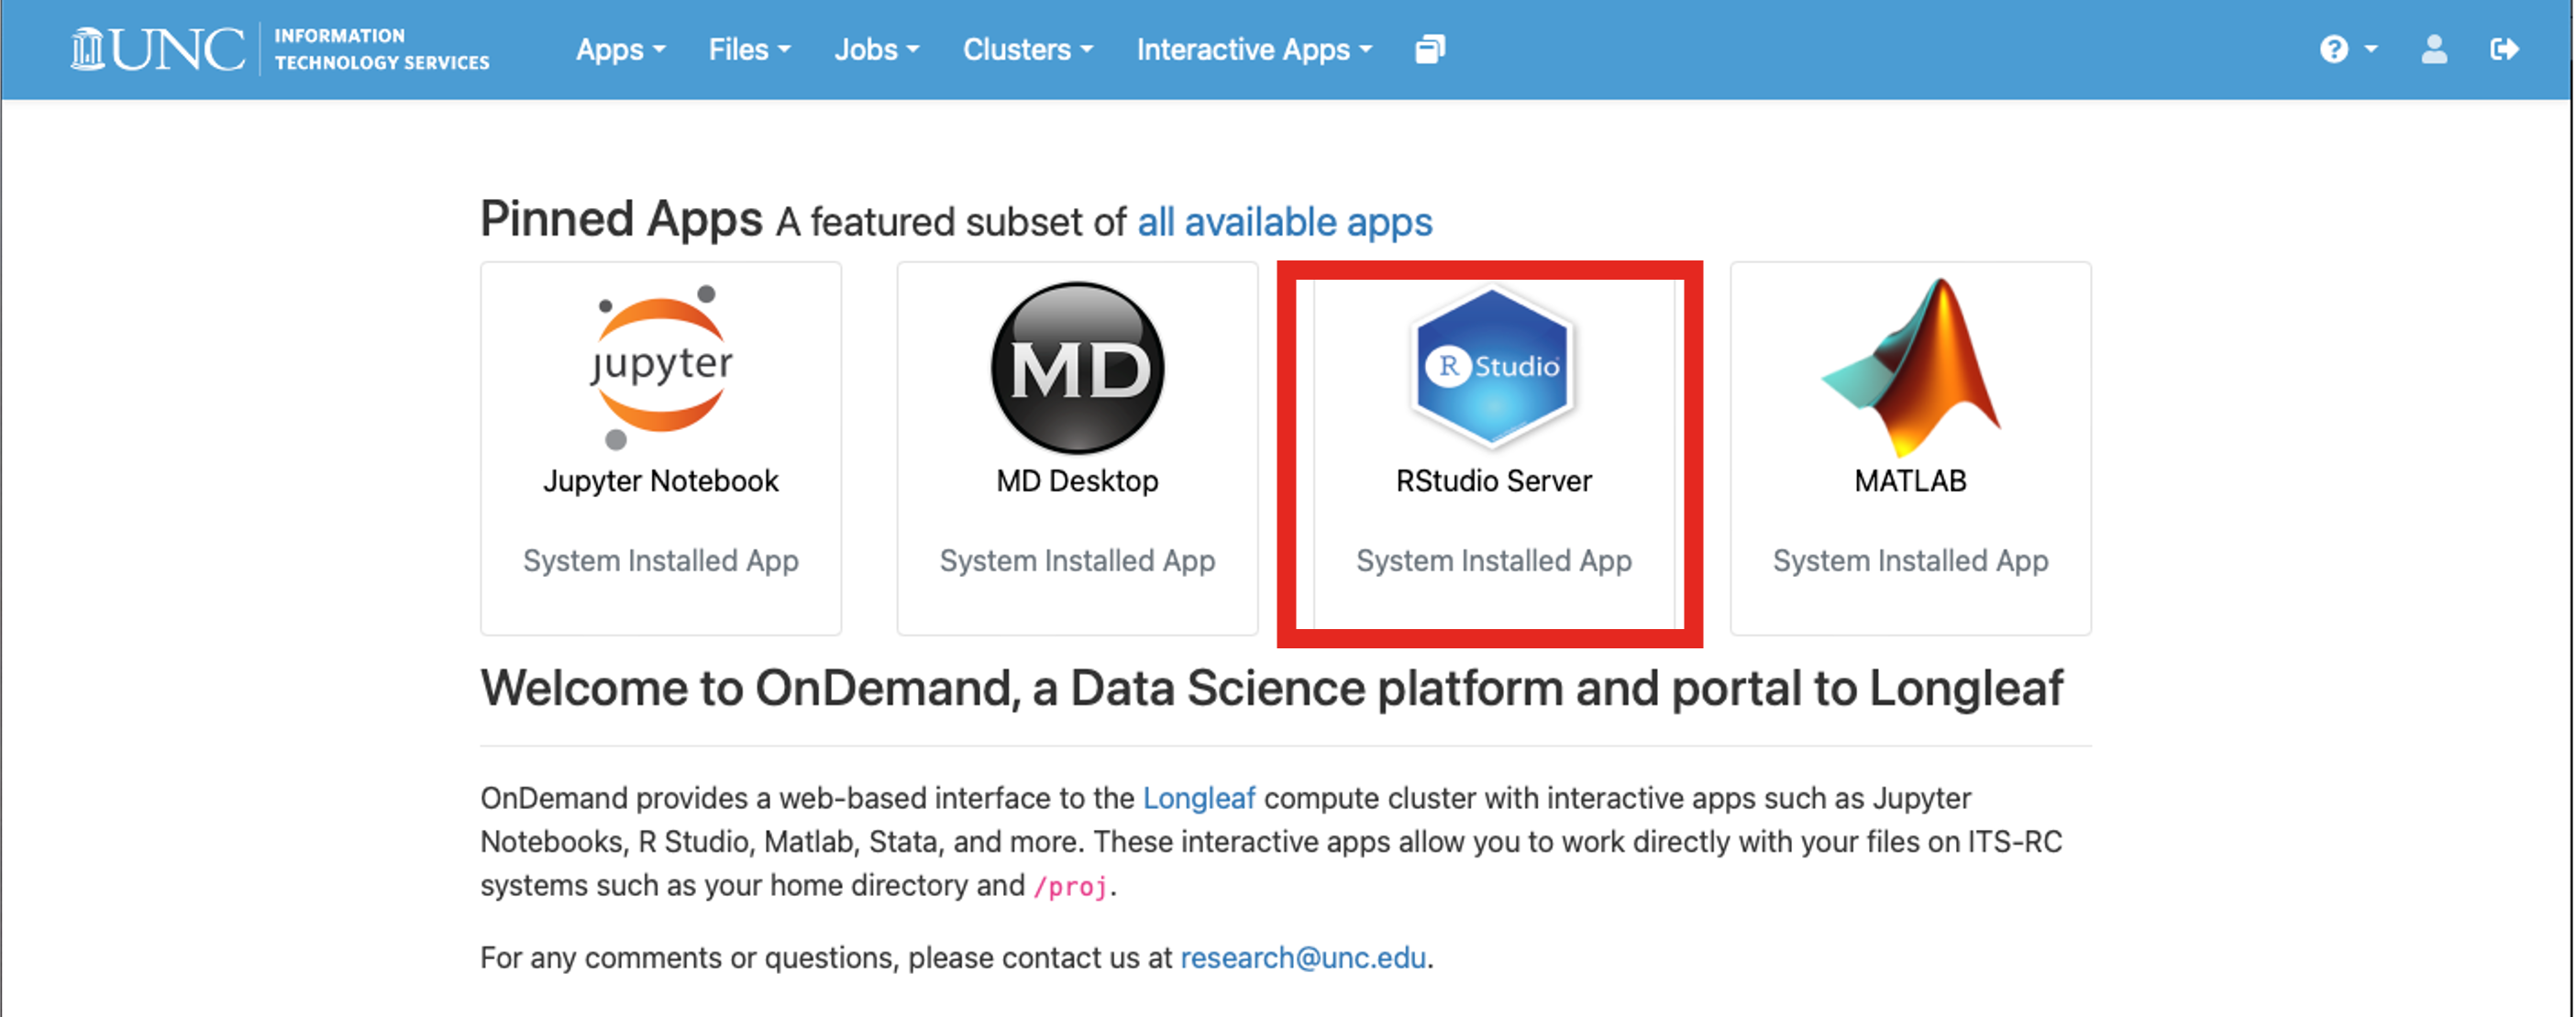
\includegraphics{scripts/00_intro/class0_images/Picture1.png}
\end{center}

This will take you to a page where you can fill out some parameters for
your R Studio Server session. The only one you'll need to adjust is
``Number of hours'' where you should put ``2''.

\begin{center}
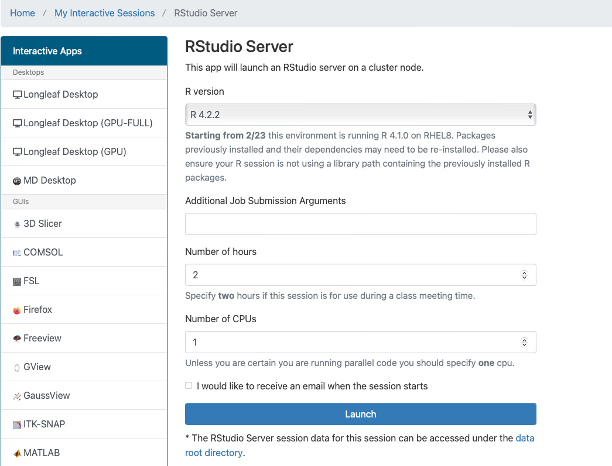
\includegraphics{scripts/00_intro/class0_images/Picture2.png}
\end{center}

\begin{tcolorbox}[enhanced jigsaw, bottomtitle=1mm, bottomrule=.15mm, toprule=.15mm, opacityback=0, leftrule=.75mm, breakable, colback=white, toptitle=1mm, left=2mm, coltitle=black, titlerule=0mm, opacitybacktitle=0.6, title=\textcolor{quarto-callout-note-color}{\faInfo}\hspace{0.5em}{Note}, rightrule=.15mm, arc=.35mm, colframe=quarto-callout-note-color-frame, colbacktitle=quarto-callout-note-color!10!white]

You can request up to 10 hours, but it's good practice to only request
the amount of time you'll need (Longleaf is a shared resource!). Since
each class is 90 minutes, you'll likely only need to request 2 hours for
each class. Under ``Additional job submission arguments'' you adjust the
amount of memory requested. This won't be needed for How to Learn to
Code classes, but may be needed when you are running your own analyses
on large datasets in the future.

\end{tcolorbox}

After you've filled out the appropriate information, click Launch. This
will take you to the ``My Interactive Sessions'' page. Your session
request may be queued for a minute while space on the cluster is being
allocated for your session. Once it's ready, click ``Connect to R Studio
Server''. This will launch R Studio in a new tab.

\begin{center}
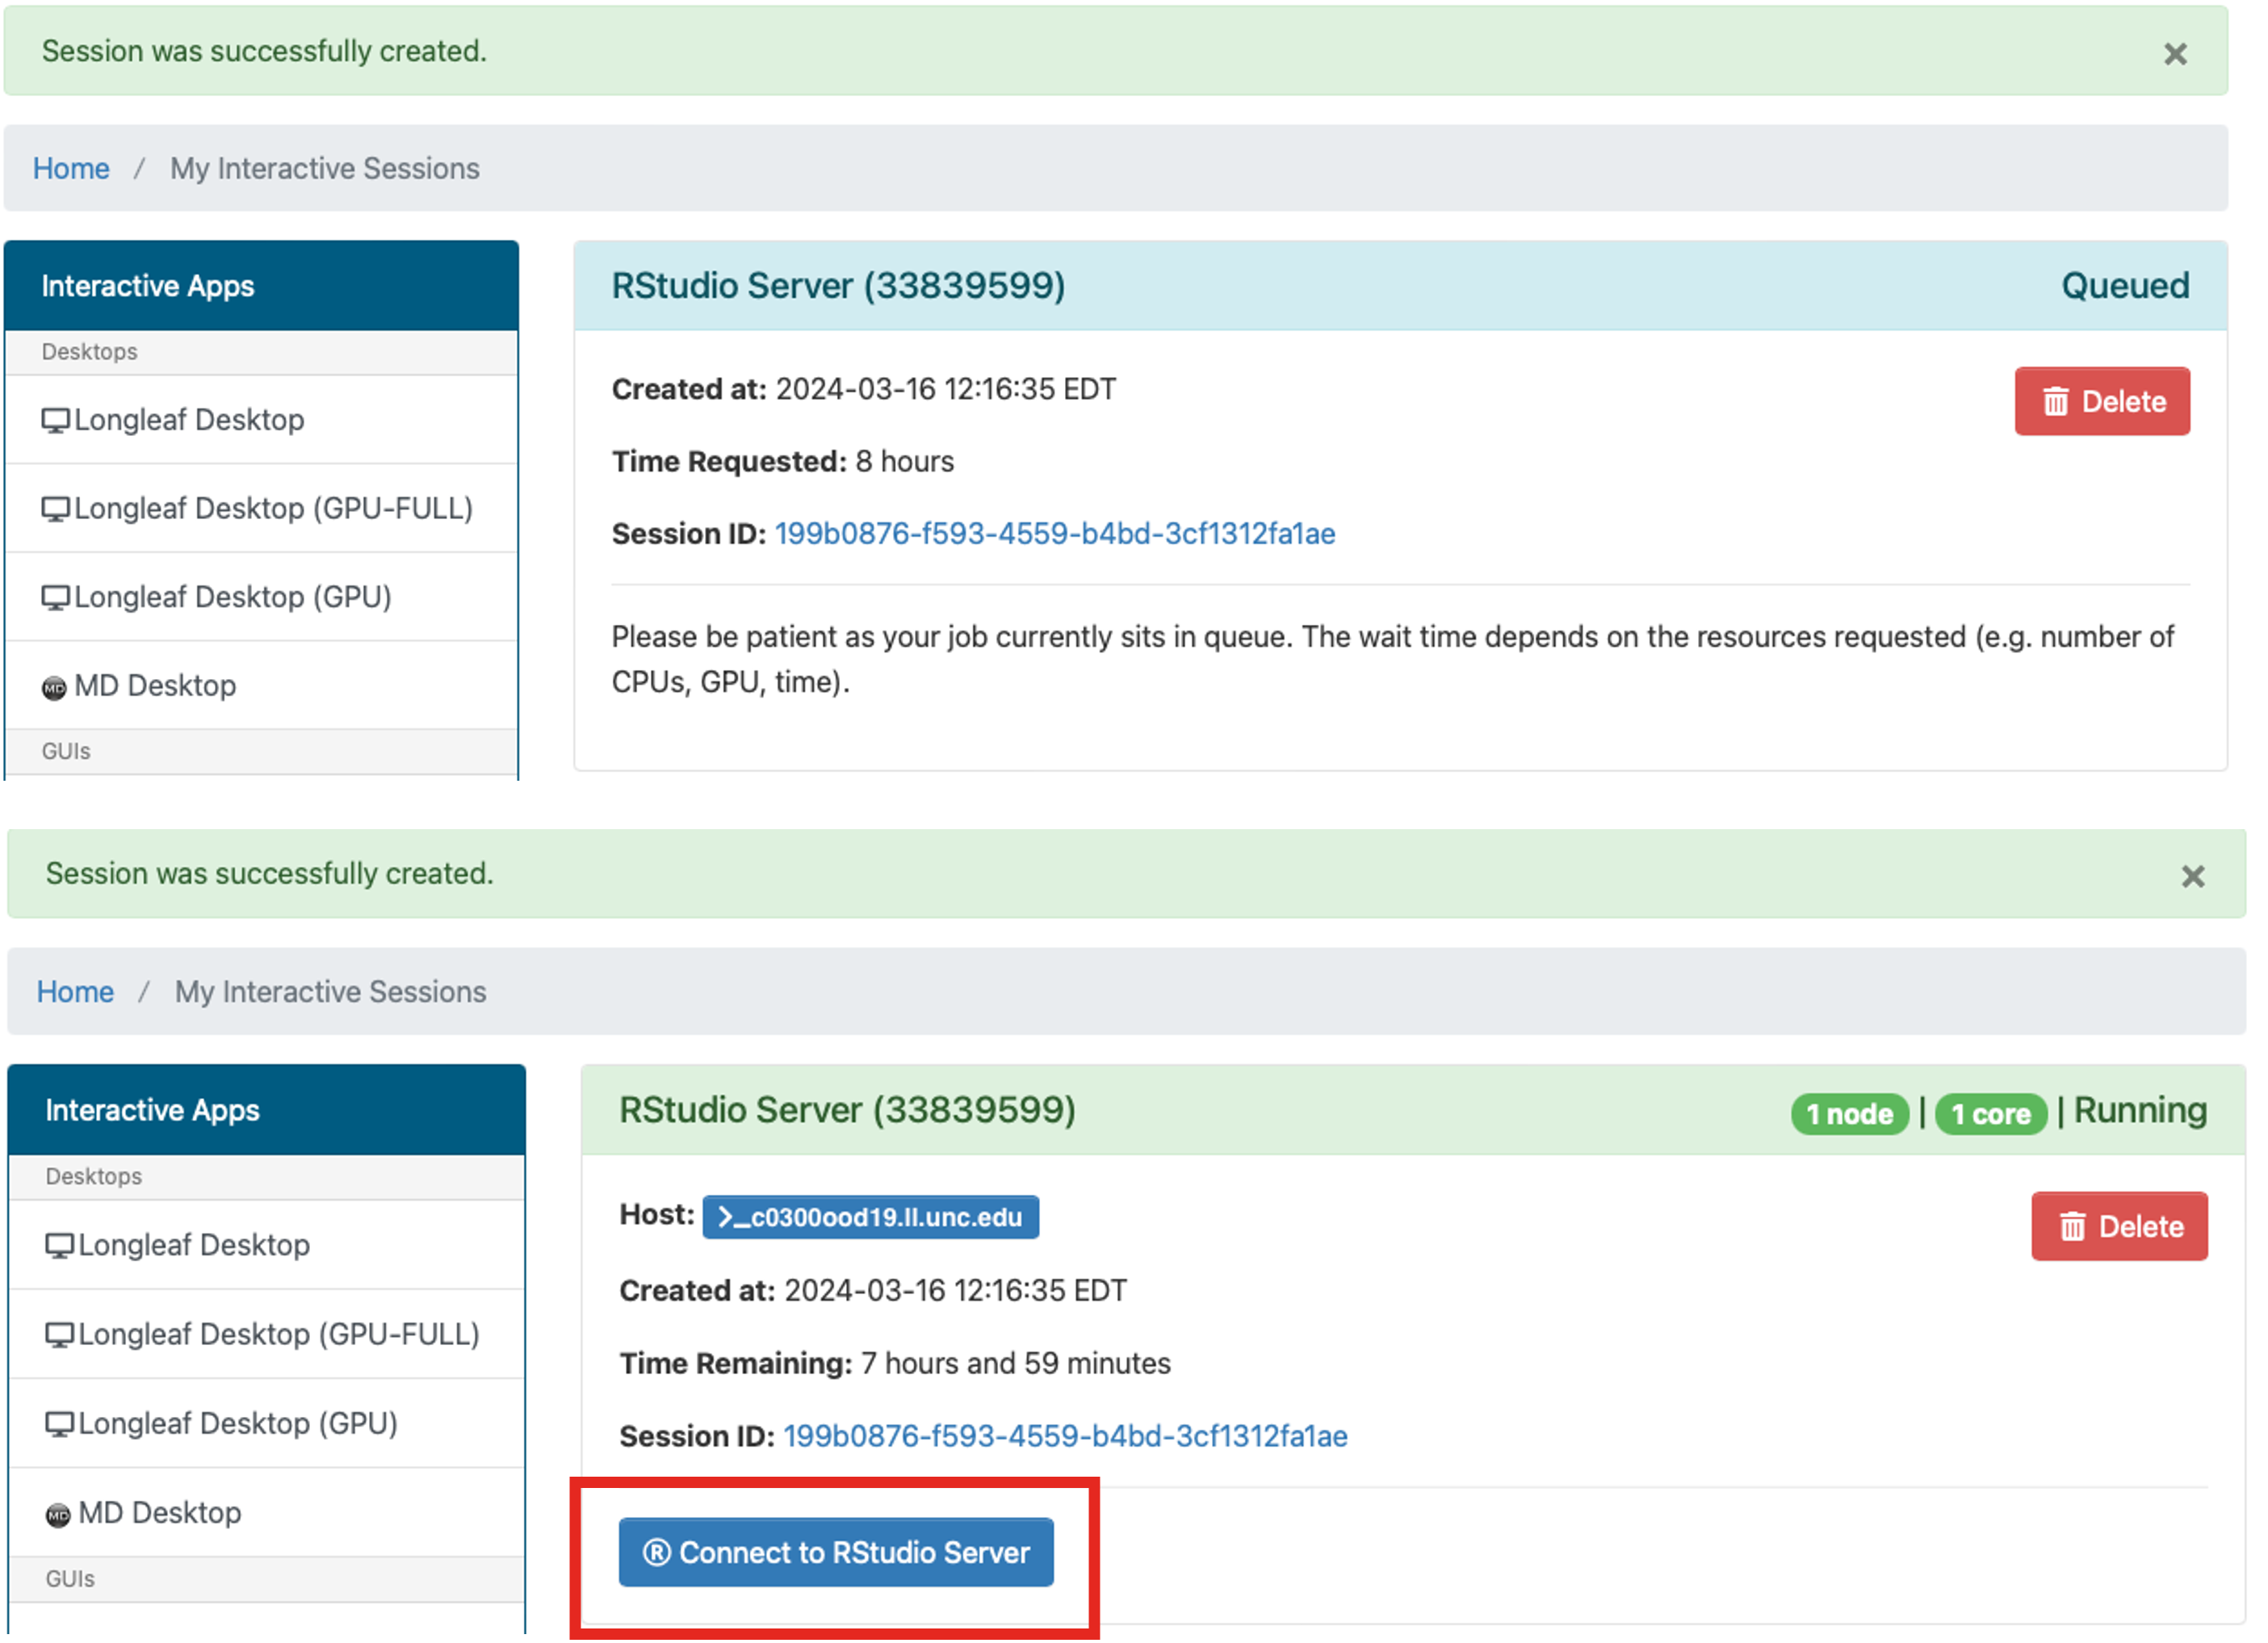
\includegraphics{scripts/00_intro/class0_images/Picture3.png}
\end{center}

\section{Navigating R Studio}\label{navigating-r-studio}

Your R Studio window is divided into four panes. You can adjust the
sizes of each pane (horizontally and vertically) by dragging the outer
edges.

\begin{tcolorbox}[enhanced jigsaw, bottomtitle=1mm, bottomrule=.15mm, toprule=.15mm, opacityback=0, leftrule=.75mm, breakable, colback=white, toptitle=1mm, left=2mm, coltitle=black, titlerule=0mm, opacitybacktitle=0.6, title=\textcolor{quarto-callout-note-color}{\faInfo}\hspace{0.5em}{Note}, rightrule=.15mm, arc=.35mm, colframe=quarto-callout-note-color-frame, colbacktitle=quarto-callout-note-color!10!white]

You may only see three panes when you first launch R Studio. If that's
the case, go to File \textgreater{} New File \textgreater{} R Script.

\end{tcolorbox}

\begin{figure}[H]

{\centering \includegraphics{index_files/mediabag/rstudio-panes-labele.jpg}

}

\caption{image:
https://docs.posit.co/ide/user/ide/guide/ui/ui-panes.html}

\end{figure}%

The top left pane is called the \textbf{Source} and this is where you
will be writing and editing code. Writing code here does not
automatically \textbf{execute} or \textbf{run} it. To do that, you will
need to use the \textbf{Console} pane in the bottom left. There are a
few ways to get code written in the Source pane to the Console pane, in
order from least efficient to most efficient:

\begin{itemize}
\item
  Copying the line of code you want to run and pasting it into the
  console and then hitting the ``return'' or ``enter'' key.
\item
  Putting your cursor anywhere in the line of code you want to run and
  clicking ``Run'' in the upper right section of the Source pane
\item
  Highlighting the line of code (or section of code) you want to run and
  clicking ``Run'' in the upper right section of the Source pane
\item
  Putting your cursor anywhere in the line of code you want to run,
  highlighting the line of code, or highlighting the section of code you
  want to run and pressing Alt + Enter (for PC) or cmd + return (for
  Mac)
\end{itemize}

Any code written in the console is \textbf{not} saved anywhere.
Generally, people write their code in the Source pane, and then run it
as needed in the Console. This is important to remember when writing
reproducible code--all code needed to run your analyses, generate plots,
etc. should be written in the source (which is then saved as an R
script). Throughout this course, you will likely want to ensure that the
code you write during each class is saved in a separate R script.

The \textbf{Environments} pane shows current saved \textbf{objects}, but
also has tabs to show history (all commands executed in your current
session) and connections (if you connect to any local or remote
databases). You will almost exclusively be using the Environment tab.
The \textbf{Output} pane is in the bottom right and shows outputs of
code such as plots. It also has tabs for files (an interactive file
explorer), packages (which shows currently installed R packages), and
help (which shows package documentation). You will likely be using the
Plots and Help tabs the most.

\section{Running code}\label{running-code}

Try running the below line of code using one of the four ways described
above. First, copy the below line of code and paste it into the Source
pane.

\texttt{print("hello\ world!")}

Before executing the code, your Source and Console panes will look like
this:

\begin{center}
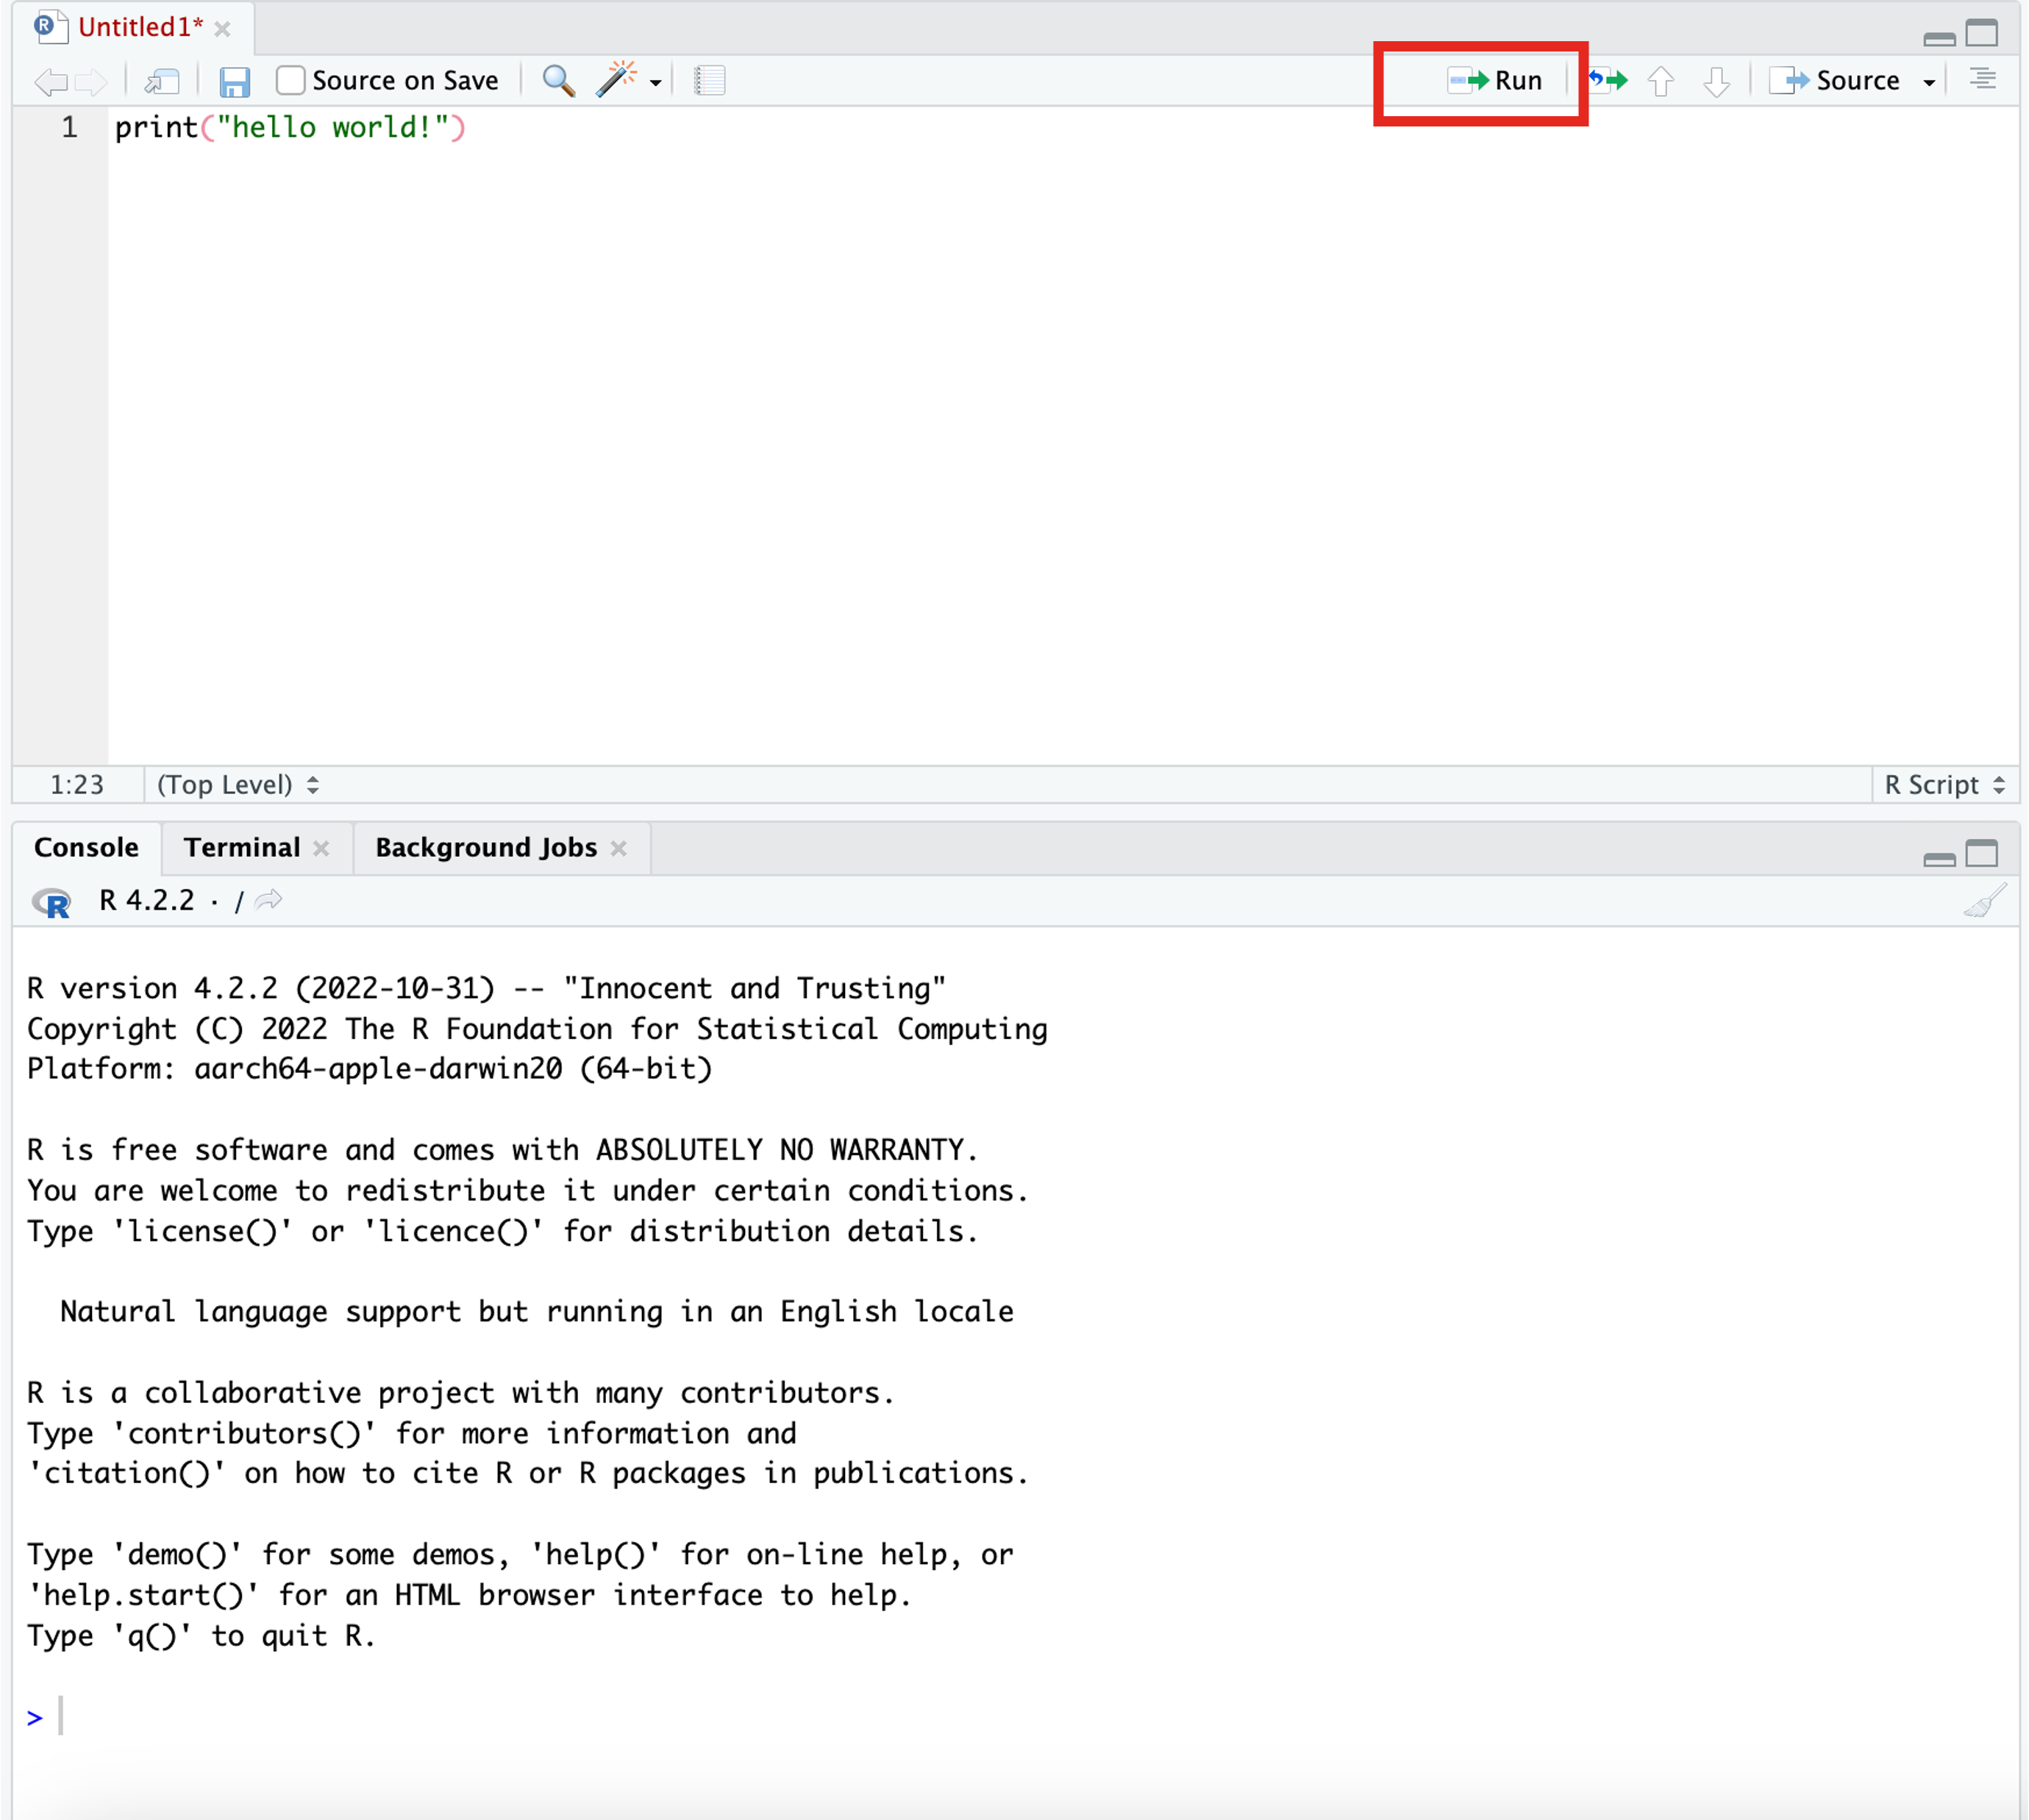
\includegraphics{scripts/00_intro/class0_images/Picture4.png}
\end{center}

After executing the line of code, your source pane will look like this:

\begin{center}
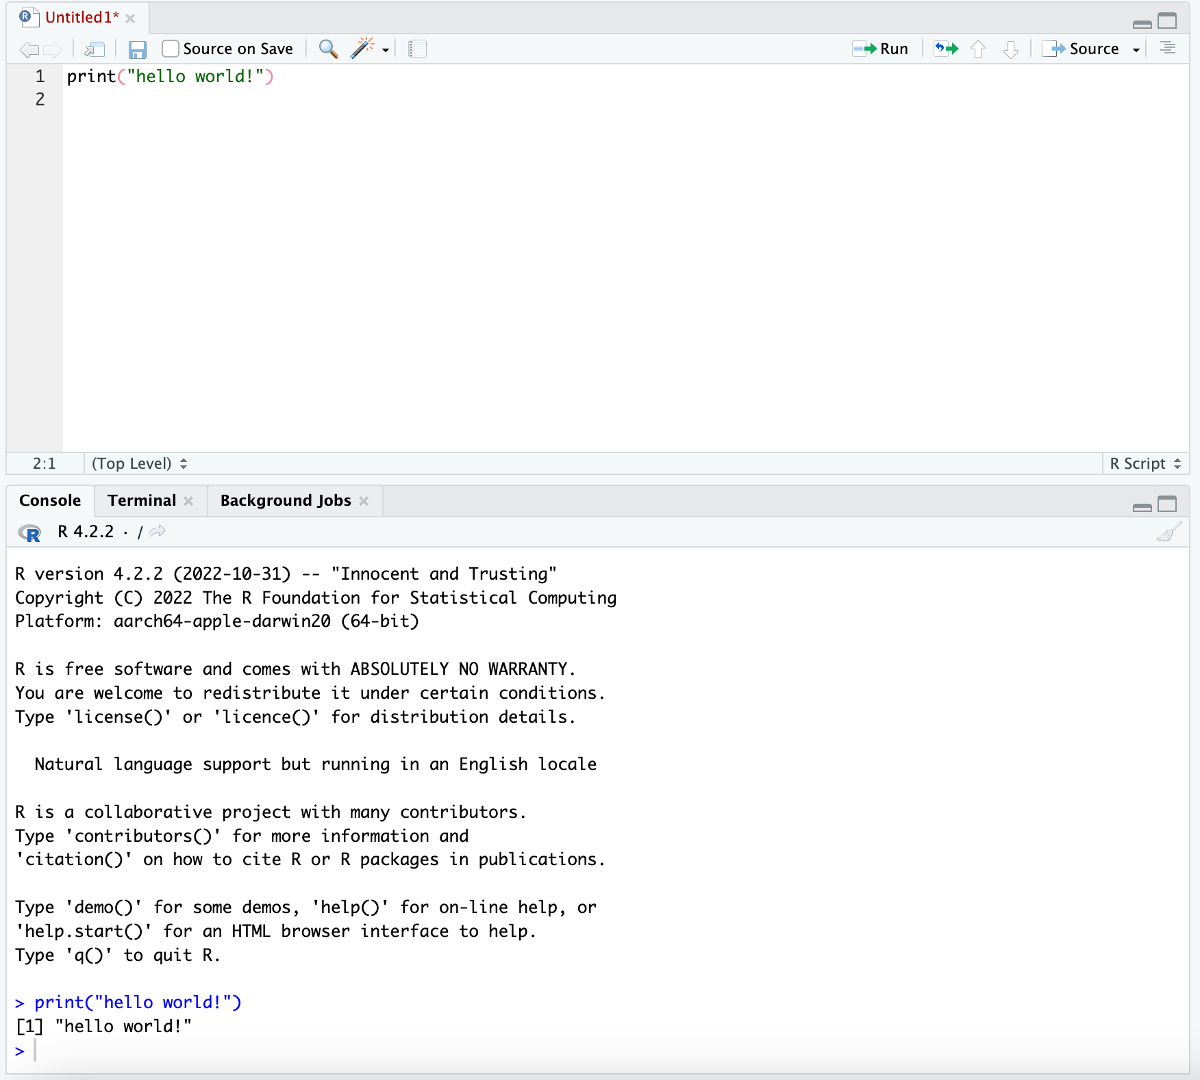
\includegraphics{scripts/00_intro/class0_images/Picture5.png}
\end{center}

Congrats! You just ran your first line of code. If you want to save your
script (what's written in the source pane) go to File \textgreater{}
Save as and save your script with a helpful name in a location that
makes sense (e.g., maybe in a folder called ``H2L2C\_class'' and name
the script ``hello\_world.R'').

Review the rest of the information on this page before Class 1, but
don't worry if it doesn't make sense right away. We will be going over
some of it in the first class and touching on it throughout the course.

\section{Talking like an R user}\label{talking-like-an-r-user}

Below is some jargon that you may hear during class. Don't worry about
memorizing it all before Class 1! Just know that it's here so if you are
ever wondering what a term means you will know where to look.

\textbf{Running code/run this line/execute:} Telling R to perform the
command given in a console. If someone says ``run this line of code''
that means to send it to the console (either by copying/pasting or using
one of the shortcuts mentioned previously).

\textbf{Data types:} Data types in R include numeric, logical, and
character. There are a few more, but those are the main three. We will
touch on these more in Classes 1 and 2.

\textbf{Vector:} A series of values of any data type. A vector is
created using the \texttt{c()} function (c for combine/concatenate).

\textbf{Factors:} This is the R term for categorical data. Sometimes R
will automatically treat data as categorical (especially if it is a
character type), but not always. You can coerce other data types (like
numeric) to factors using using the \texttt{factor()} function and
specifying the order using the \texttt{levels} argument. For more
information on factors, see
\href{https://r4ds.hadley.nz/factors.html}{this page} in the R for Data
Science book.

\textbf{Data frame:} The best way to think of data frames is a
spreadsheet. Technically, they are composed of vectors. Typically the
rows in a data frame will correspond to observations and the columns
will correspond to variables describing those observations. Data in a
data frame can be of different types--i.e.~you can have one column be
character (maybe describing hair color for each observation) and another
be numeric (maybe describing height for each observation).

\textbf{Matrix:} A matrix in R is very similar to a data frame. Unlike a
data frame, all elements must be of the same data type.

\textbf{Functions:} A function performs a given task. This task can be
very simple (add two numbers) or more complex (create a large data
frame, run a linear regression, save the output to a csv file). R has
many built-in functions you will use. Many packages also have functions
you can use.

\textbf{Packages:} Packages in R are extensions of what is called ``base
R.'' Base R refers to using R without any add-ons (i.e., no packages).
Packages can have data, functions, and/or compiled code. It is the
responsibility of package developers to maintain their package--which
means some undergo frequent updates and some haven't been touched in
years (and thus might not work anymore for whatever reason). It also
means that some packages can have bugs or might not be appropriate for
your data/analysis. To use a package, you will first need to install it
using the function
\texttt{install.package("\textless{}package\_name\textgreater{}")}. You
will only need to install the package once. Each time you want to use
the package, you'll need to load it into your environment:
\texttt{library(\textless{}package\_name\textquotesingle{})}. Once it is
loaded into your environment, you will be able to use any functions or
data in the package.

\textbf{global vs.~local:} Global refers to something (usually a
variable) that is accessible to the entire program/code. Local refers to
something (usually a variable) that is accessible only relative to
something else (such as within a specific code block, like a function).

\begin{Shaded}
\begin{Highlighting}[]
\CommentTok{\# Global variable}
\NormalTok{x }\OtherTok{\textless{}{-}} \StringTok{"airplane"}
\CommentTok{\# Function that defines a local variable}
\NormalTok{my\_function }\OtherTok{\textless{}{-}} \ControlFlowTok{function}\NormalTok{() \{}
\NormalTok{    y }\OtherTok{\textless{}{-}} \StringTok{"car"}
\NormalTok{\}}
\CommentTok{\# Accessing the local variable outside the function returns an error}
\NormalTok{y}
\CommentTok{\# But the global variable is accessible}
\NormalTok{x}
\CommentTok{\# Accessing the local variable }
\NormalTok{z }\OtherTok{\textless{}{-}} \FunctionTok{my\_function}\NormalTok{()}
\NormalTok{z}
\end{Highlighting}
\end{Shaded}

\textbf{directory:} A directory is another term for what you may refer
to as a ``folder'' on your computer.

\textbf{paths:} Paths are the directions to files and folders on your
system. Understanding paths is important for reading your data into your
R environment, since you will need to tell R where the file is located.
You can have global and local paths. Global paths are sort of like the
full set of instructions starting from your home base. Local paths are
instructions given a certain starting location. Here's an example of a
global path to an example file on Longleaf:
\texttt{/work/users/g/h/goheels/my\_project/my\_data.csv}. Here's an
example of a local path, given the starting spot of the \texttt{goheels}
directory: \texttt{my\_project/my\_data.csv}.

\textbf{syntax/style:} The visual appearance (spaces, indentations,
capitalization) of your code greatly improves readability and makes it
easier for someone else to quickly understand what it's doing (or you
six months later). In this class, we will follow the Tidyverse Style
Guide and encourage you to reference it during class to ensure you are
consistently naming variables and using appropriate syntax. The sections
most relevant for now are
\href{https://style.tidyverse.org/files.html}{Files},
\href{https://style.tidyverse.org/files.html}{Syntax}, and the
``Comments'' section of the
\href{https://style.tidyverse.org/functions.html\#comments-1}{Functions}
page. Later classes will touch on
\href{https://style.tidyverse.org/pipes.html}{pipes} and
\href{https://style.tidyverse.org/ggplot2.html}{ggplot2}.

\textbf{Conditionals:} A conditional is a line of code that will run
only if a particular condition is met. You can recognize these by the
use of ``if'' ``else'' or ``while''. The best way to understand these is
by actually reading the code out loud. If you were to read the below
example out loud, you might say ``if x equals 3, print `condition is
met', else print `condition is not met'\,''. What do you think will
happen if \texttt{x\ ==\ 3}? What if \texttt{x\ ==\ 4}?

\begin{Shaded}
\begin{Highlighting}[]
\ControlFlowTok{if}\NormalTok{(x }\SpecialCharTok{==} \DecValTok{3}\NormalTok{) \{}
  \FunctionTok{print}\NormalTok{(}\StringTok{"condition is met"}\NormalTok{)}
\NormalTok{\} }\ControlFlowTok{else}\NormalTok{ \{}
  \FunctionTok{print}\NormalTok{(}\StringTok{"condition is not met"}\NormalTok{)}
\NormalTok{\}}
\end{Highlighting}
\end{Shaded}

\section{Understanding errors and
warnings}\label{understanding-errors-and-warnings}

You will get lots of errors during your How to Learn to Code Journey.
``Warnings'' indicate your code ran, but some non-fatal issue arose.
Sometimes these are OK to ignore, sometimes they indicate an issue you
need to look into further. Either way, they should always be
investigated! ``Errors'' are fatal issues and may be the result of
things like syntax errors, typos, and incorrect data types. A good
starting point for investigating any error or warning is Google (chances
are quite high someone has run into the same issue, especially when
you're just learning how to code). You can copy and paste the entire
error/warning into Google and usually return a helpful result.

\section{Use of AI tools}\label{use-of-ai-tools}

Using AI tools such as ChatGPT and Microsoft Copilot can be really
helpful! But before turning to these tools for assistance, try figuring
out the solution yourself. Part of learning how to code is learning how
to \emph{think} like a coder, and that requires doing things the hard
way for a bit. Remember that you are responsible for understanding what
your code is doing and why, and that the output is accurate.
Additionally, depending on the type of work you are doing, you many need
to use additional caution when copying and pasting code/data (any
questions/concerns on this should be directed to your PI/department).

\section{I'm stuck! Additional
resources}\label{im-stuck-additional-resources}

Research IT page on how to use OnDemand:
\url{https://help.rc.unc.edu/ondemand}

Getting started on Longleaf:
\url{https://help.rc.unc.edu/getting-started-on-longleaf}

More stats please!
\url{https://odum.unc.edu/education/short-courses/\#course1}

Still haven't found what you're looking for? Post a message in the How
to Learn to Code Teams!

\section{Bonus: Installing R Studio on your personal
computer}\label{bonus-installing-r-studio-on-your-personal-computer}

A lot of you may want to use R on your personal computer (i.e., not on
Longleaf). There may be reasons why you want to stick with Longleaf
though (e.g., data should not be downloaded on personal devices,
data/analysis requires a lot of memory). If you are interested in
installing R and R Studio on your personal computer, you can use the
below resources for help. All classes will be taught assuming you are
using Longleaf though, so class time won't be dedicated to
troubleshooting R install issues on personal computers.

If you just want to click 2 buttons and figure it out:
\url{https://posit.co/download/rstudio-desktop/}

If you want a more detailed install walkthrough:
\url{https://rstudio-education.github.io/hopr/starting.html}

\bookmarksetup{startatroot}

\chapter{R Coding Basics}\label{r-coding-basics}

Coding Basics, Day 1

\hfill\break

\section{Introduction}\label{introduction-1}

\begin{quote}
Many biologists starting out in bioinformatics tend to equate ``learning
bioinformatics'' with ``learning how to run bioinformatics
software''\ldots{} This is analogous to thinking ``learning molecular
biology'' is just ``learning pipetting.''

--- Vince Buffalo
\end{quote}

In Vince's quote above, replace ``bioinformatics'' with ``coding.''

Our goal for How to Learn to Code is to familiarize students with the R
programming language and RStudio environment, equip students with the
skills and knowledge to wrangle, visualize, and analyze data, and to
provide a foundation for more advanced coding skills.

In Module 1: Coding Basics, we will cover:

\begin{itemize}
\tightlist
\item
  Variables
\item
  Reproducible environments
\item
  RStudio IDE
\item
  Various R script and file formats
\item
  R syntax
\item
  Commenting, writing, and executing code
\item
  Functions
\item
  Data structures in R
\item
  Data types in R
\item
  Manipulating data types and structures
\end{itemize}

Curious about what the rest of the classes will look like?

\begin{itemize}
\item
  Module 1: Coding Basics
\item
  Module 2: Data Visualization
\item
  Module 3: Data Wrangling
\item
  Module 4: Project Management (and applying everything you've learned
  to a real-world dataset!)
\end{itemize}

\section{Objectives of Coding Basics: Class
1}\label{objectives-of-coding-basics-class-1}

\begin{itemize}
\item
  Be able to create a variable, define what it is, and follow good
  variable naming practices
\item
  Understand basic data structures in R
\item
  Understand basic data types in R
\item
  Perform basic manipulations with data structures and types
\item
  Describe benefits of knowing how to code
\end{itemize}

\section{Exploring a dataset}\label{exploring-a-dataset}

R has a few built in datasets that we can use until we cover
installing/loading packages and reading in data files. For the following
examples we will use a built-in dataset in R called ``iris'' that has
some measurements across a few species of flowers. It is one of the most
popular built-in datasets in R. We will use this dataset to explore key
coding concepts: \textbf{variables}, \textbf{data types}, and
\textbf{functions}.

First, let's take a look at the dataset. You can view the dataset
multiple ways. Let's try one--copy the below line of code into your
console and run it.

\begin{Shaded}
\begin{Highlighting}[]
\NormalTok{iris}
\end{Highlighting}
\end{Shaded}

As we can see, this dataset has a few columns of numbers, in addition to
the species. Let's try a few other ways to look at this dataset. As you
try each method, think about what is different about each method. When
would one method be more beneficial than another?

\begin{Shaded}
\begin{Highlighting}[]
\FunctionTok{head}\NormalTok{(iris)}
\end{Highlighting}
\end{Shaded}

\begin{verbatim}
  Sepal.Length Sepal.Width Petal.Length Petal.Width Species
1          5.1         3.5          1.4         0.2  setosa
2          4.9         3.0          1.4         0.2  setosa
3          4.7         3.2          1.3         0.2  setosa
4          4.6         3.1          1.5         0.2  setosa
5          5.0         3.6          1.4         0.2  setosa
6          5.4         3.9          1.7         0.4  setosa
\end{verbatim}

\begin{Shaded}
\begin{Highlighting}[]
\FunctionTok{View}\NormalTok{(iris)}
\end{Highlighting}
\end{Shaded}

You are probably already thinking of questions you need the answers to
in order to familiarize yourself with this dataset. What does each row
represent? Each column? How many observations (rows) do we have? What is
the average petal length? Think about other questions you may want to
ask. Think about how you would go about answering those questions with
what you already know. Maybe you'd count each row on your screen to get
the number of observations, or copy the values under
\texttt{Petal.Length} into your phone calculator to calculate the mean.
By the end of this class, you'll be able to do all those things very
quickly in R!

\section{Variables}\label{variables}

A variable is a named space in your computer's memory which can be
referenced and manipulated. It's sort of a name you give ``something'',
and that something can be just about anything.

\begin{figure}[H]

{\centering 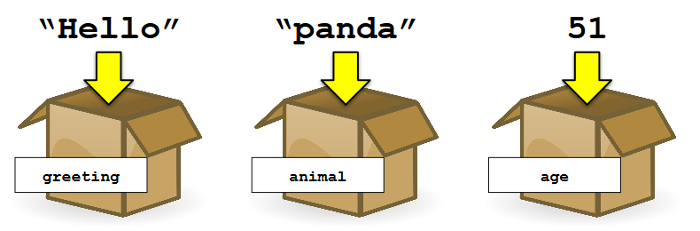
\includegraphics{scripts/01_codingBasics/class1-files/variables.png}

}

\caption{https://mclark45.medium.com/variables-8d0ba47d9694}

\end{figure}%

Variables in R are created (assigned) using an arrow:
\texttt{\textless{}-} The variable name always goes on the left, and the
thing being assigned to that variable on the right. For example:

\begin{Shaded}
\begin{Highlighting}[]
\NormalTok{greeting }\OtherTok{\textless{}{-}} \StringTok{"Hello"}
\NormalTok{animal }\OtherTok{\textless{}{-}} \StringTok{"panda"}
\NormalTok{age }\OtherTok{\textless{}{-}} \DecValTok{51}
\end{Highlighting}
\end{Shaded}

The value something is assigned to is often referred to as the variable
name. For example, the variable name of \texttt{"Hello"} is
\texttt{greeting} . We used really basic variable names--just letters,
that are real words, all lowercase. Of course, there are other ways to
name variables too! Play around with variable names. Try using uppercase
letters, symbols, and numbers. What works, and what doesn't? Come up
with some rules for variable naming. Here's some variable naming ideas
to get you started:

\begin{Shaded}
\begin{Highlighting}[]
\NormalTok{GrEeTiNg }\OtherTok{\textless{}{-}} \StringTok{"Hello"}
\DecValTok{5}\NormalTok{greeting }\OtherTok{\textless{}{-}} \StringTok{"Hello"}
\NormalTok{greeting}\FloatTok{.5} \OtherTok{\textless{}{-}} \StringTok{"Hello"}
\NormalTok{greeting}\SpecialCharTok{@}\DecValTok{5} \OtherTok{\textless{}{-}} \StringTok{"Hello"}
\end{Highlighting}
\end{Shaded}

Now that you know some general rules for variable naming, we can refer
to the \href{https://style.tidyverse.org/syntax.html\#syntax}{Style
Guide} for ``proper'' variable/object naming. Update your variable
naming rule to include the preferred style for variable names according
to the Style Guide.

And now that we know how to properly name variables, assign the iris
dataset to a variable!

\begin{Shaded}
\begin{Highlighting}[]
\NormalTok{iris\_dataset\_copy }\OtherTok{\textless{}{-}}\NormalTok{ iris}
\end{Highlighting}
\end{Shaded}

\section{Data types}\label{data-types}

As you probably know from your own work, data can come in many forms.
You can classify dragons as either ``purple'' or ``green'' and also
record the number of spines on their backs as numeric types (15, 27).
Data types are important to understand in R because the type of data
impacts what you can do with that data. For example, it wouldn't make
sense to calculate a mean for the dragon color, but it would for the
number of back spines.

In R, we will focus on three basic data types that are used specify the
type of data stored in a variable (there are a few more, but you
probably won't ever run into them): \textbf{character, numeric,} and
\textbf{logical.}

\textbf{Character:} A character represents a string value. This can be
anything from a single letter to entire paragraphs. Examples include
\texttt{“a”,\ “B”,\ “c\ is\ third”,\ "5"}

\textbf{Numeric:} A decimal value. Examples include
\texttt{1.0,\ 3.1415926535}.

\textbf{Logical:} Logical data types have only two possible values:
\texttt{TRUE} or \texttt{FALSE}.

So far, we have learned about basic data structures (vectors, matrices,
etc.) and basic data types (numeric, character, logical). Now, we want
to start manipulating or \emph{doing things} to them that can be
helpful.

\section{Converting Data Types}\label{converting-data-types}

For example, sometimes when we read in data from a file, numbers can
appear as strings of characters rather than a ``numeric'' type.

\begin{Shaded}
\begin{Highlighting}[]
\NormalTok{my\_numbers }\OtherTok{\textless{}{-}} \FunctionTok{c}\NormalTok{(}\StringTok{"4"}\NormalTok{, }\StringTok{"2"}\NormalTok{, }\StringTok{"7"}\NormalTok{, }\StringTok{"10"}\NormalTok{)}
\FunctionTok{print}\NormalTok{(my\_numbers)}
\end{Highlighting}
\end{Shaded}

\begin{verbatim}
[1] "4"  "2"  "7"  "10"
\end{verbatim}

How can we tell? Because the numbers above are in quotations, indicating
that they are of the \texttt{character} type and R is interpreting them
as text. Before doing any math or further analysis with these data
points, it's a good idea to convert them to the \texttt{numeric} type
first.

\begin{Shaded}
\begin{Highlighting}[]
\NormalTok{my\_numbers }\OtherTok{\textless{}{-}} \FunctionTok{as.numeric}\NormalTok{(my\_numbers)}
\FunctionTok{print}\NormalTok{(my\_numbers)}
\end{Highlighting}
\end{Shaded}

\begin{verbatim}
[1]  4  2  7 10
\end{verbatim}

Note that the quotations are now gone. Now, we can do basic (or more
advanced) calculations like the ones below.

\begin{Shaded}
\begin{Highlighting}[]
\CommentTok{\# Get minimum out of a list of values}
\FunctionTok{min}\NormalTok{(my\_numbers)}
\end{Highlighting}
\end{Shaded}

\begin{verbatim}
[1] 2
\end{verbatim}

\begin{Shaded}
\begin{Highlighting}[]
\CommentTok{\# Get maximum out of a list of values}
\FunctionTok{max}\NormalTok{(my\_numbers)}
\end{Highlighting}
\end{Shaded}

\begin{verbatim}
[1] 10
\end{verbatim}

\begin{Shaded}
\begin{Highlighting}[]
\CommentTok{\# Get average (mean) out of a list of values}
\FunctionTok{mean}\NormalTok{(my\_numbers)}
\end{Highlighting}
\end{Shaded}

\begin{verbatim}
[1] 5.75
\end{verbatim}

We can also sort this list of values to go from smallest to largest.
After doing so, the smallest value will be first in the list and the
largest value will be last.

\begin{Shaded}
\begin{Highlighting}[]
\NormalTok{my\_numbers }\OtherTok{\textless{}{-}} \FunctionTok{sort}\NormalTok{(my\_numbers)}
\NormalTok{my\_numbers}
\end{Highlighting}
\end{Shaded}

\begin{verbatim}
[1]  2  4  7 10
\end{verbatim}

We can reverse the order to go from largest to smallest. There is an
option using the \texttt{sort} function to do this.

\begin{Shaded}
\begin{Highlighting}[]
\NormalTok{my\_numbers }\OtherTok{\textless{}{-}} \FunctionTok{sort}\NormalTok{(my\_numbers, }\AttributeTok{decreasing =} \ConstantTok{TRUE}\NormalTok{)}
\NormalTok{my\_numbers}
\end{Highlighting}
\end{Shaded}

\begin{verbatim}
[1] 10  7  4  2
\end{verbatim}

\section{Accessing parts of a list}\label{accessing-parts-of-a-list}

One thing we'll be doing a lot of is looking at parts of our data. For
example, we might want to look at individual items in a vector. These
items could be numbers or characters.

\begin{Shaded}
\begin{Highlighting}[]
\NormalTok{my\_data }\OtherTok{\textless{}{-}} \FunctionTok{c}\NormalTok{(}\StringTok{"A"}\NormalTok{, }\StringTok{"B"}\NormalTok{, }\StringTok{"C"}\NormalTok{, }\StringTok{"D"}\NormalTok{, }\StringTok{"E"}\NormalTok{, }\StringTok{"F"}\NormalTok{)}
\NormalTok{my\_data}
\end{Highlighting}
\end{Shaded}

\begin{verbatim}
[1] "A" "B" "C" "D" "E" "F"
\end{verbatim}

In this case, let's say I'm really interested in that ``E'' and want to
pull it out separately from the rest of the data. I can do that with
``indexing''. Here, I can tell that it's the 5th item in the list, so I
can extract it using the following:

\begin{Shaded}
\begin{Highlighting}[]
\NormalTok{my\_data[}\DecValTok{5}\NormalTok{]}
\end{Highlighting}
\end{Shaded}

\begin{verbatim}
[1] "E"
\end{verbatim}

We can also extract multiple items. If we wanted ``D'', ``E'', and
``F'', we can get all the values from item 4 (``D'') to item 6 (``F'').

\begin{Shaded}
\begin{Highlighting}[]
\NormalTok{my\_data[}\DecValTok{4}\SpecialCharTok{:}\DecValTok{6}\NormalTok{]}
\end{Highlighting}
\end{Shaded}

\begin{verbatim}
[1] "D" "E" "F"
\end{verbatim}

Let's say we forgot to include some of our data and now we want to add
it to this list. We can update \texttt{my\_data} to also include these
values.

\begin{Shaded}
\begin{Highlighting}[]
\NormalTok{my\_data }\OtherTok{\textless{}{-}} \FunctionTok{c}\NormalTok{(my\_data, }\StringTok{"G"}\NormalTok{, }\StringTok{"H"}\NormalTok{, }\StringTok{"I"}\NormalTok{)}
\NormalTok{my\_data}
\end{Highlighting}
\end{Shaded}

\begin{verbatim}
[1] "A" "B" "C" "D" "E" "F" "G" "H" "I"
\end{verbatim}

Before we move on, let's cover creating vectors. We already did this
several times above, but didn't discuss it. Typically, we'll want to
make vectors of numbers (e.g.~our data values) or vectors of characters
(e.g.~labels for our data). Depending on whether we use quotes or not, R
will interpret them as either numeric vectors or character vectors.

\begin{Shaded}
\begin{Highlighting}[]
\CommentTok{\# Numeric vector}
\NormalTok{numeric\_vector }\OtherTok{\textless{}{-}} \FunctionTok{c}\NormalTok{(}\DecValTok{1}\NormalTok{, }\DecValTok{2}\NormalTok{, }\DecValTok{3}\NormalTok{, }\DecValTok{4}\NormalTok{, }\DecValTok{5}\NormalTok{)}
\NormalTok{numeric\_vector}
\end{Highlighting}
\end{Shaded}

\begin{verbatim}
[1] 1 2 3 4 5
\end{verbatim}

\begin{Shaded}
\begin{Highlighting}[]
\CommentTok{\# Character vector}
\NormalTok{character\_vector }\OtherTok{\textless{}{-}} \FunctionTok{c}\NormalTok{(}\StringTok{"apple"}\NormalTok{, }\StringTok{"banana"}\NormalTok{, }\StringTok{"orange"}\NormalTok{)}
\NormalTok{character\_vector}
\end{Highlighting}
\end{Shaded}

\begin{verbatim}
[1] "apple"  "banana" "orange"
\end{verbatim}

Remember the iris dataset from earlier? Let's return to it to cover
extracting some of the rows or columns from this data.

We can access specific columns in one of two ways. Typically, we will
want to access it by the name of the column. We do this using the name
of the data frame, followed by the dollar sign, and finally the name of
the column. For example:

\begin{Shaded}
\begin{Highlighting}[]
\NormalTok{iris}\SpecialCharTok{$}\NormalTok{Petal.Length}
\end{Highlighting}
\end{Shaded}

\begin{verbatim}
  [1] 1.4 1.4 1.3 1.5 1.4 1.7 1.4 1.5 1.4 1.5 1.5 1.6 1.4 1.1 1.2 1.5 1.3 1.4
 [19] 1.7 1.5 1.7 1.5 1.0 1.7 1.9 1.6 1.6 1.5 1.4 1.6 1.6 1.5 1.5 1.4 1.5 1.2
 [37] 1.3 1.4 1.3 1.5 1.3 1.3 1.3 1.6 1.9 1.4 1.6 1.4 1.5 1.4 4.7 4.5 4.9 4.0
 [55] 4.6 4.5 4.7 3.3 4.6 3.9 3.5 4.2 4.0 4.7 3.6 4.4 4.5 4.1 4.5 3.9 4.8 4.0
 [73] 4.9 4.7 4.3 4.4 4.8 5.0 4.5 3.5 3.8 3.7 3.9 5.1 4.5 4.5 4.7 4.4 4.1 4.0
 [91] 4.4 4.6 4.0 3.3 4.2 4.2 4.2 4.3 3.0 4.1 6.0 5.1 5.9 5.6 5.8 6.6 4.5 6.3
[109] 5.8 6.1 5.1 5.3 5.5 5.0 5.1 5.3 5.5 6.7 6.9 5.0 5.7 4.9 6.7 4.9 5.7 6.0
[127] 4.8 4.9 5.6 5.8 6.1 6.4 5.6 5.1 5.6 6.1 5.6 5.5 4.8 5.4 5.6 5.1 5.1 5.9
[145] 5.7 5.2 5.0 5.2 5.4 5.1
\end{verbatim}

If we knew which column it was (or it wasn't named), we can also use
indexing. Inside the brackets, we will need to indicate which {[}row ,
column{]} we want from this data frame. Since we want all the rows, we
will leave the ``row'' blank. We can see that the Petal.Length was the
3rd column.

\begin{Shaded}
\begin{Highlighting}[]
\NormalTok{iris[, }\DecValTok{3}\NormalTok{]}
\end{Highlighting}
\end{Shaded}

\begin{verbatim}
  [1] 1.4 1.4 1.3 1.5 1.4 1.7 1.4 1.5 1.4 1.5 1.5 1.6 1.4 1.1 1.2 1.5 1.3 1.4
 [19] 1.7 1.5 1.7 1.5 1.0 1.7 1.9 1.6 1.6 1.5 1.4 1.6 1.6 1.5 1.5 1.4 1.5 1.2
 [37] 1.3 1.4 1.3 1.5 1.3 1.3 1.3 1.6 1.9 1.4 1.6 1.4 1.5 1.4 4.7 4.5 4.9 4.0
 [55] 4.6 4.5 4.7 3.3 4.6 3.9 3.5 4.2 4.0 4.7 3.6 4.4 4.5 4.1 4.5 3.9 4.8 4.0
 [73] 4.9 4.7 4.3 4.4 4.8 5.0 4.5 3.5 3.8 3.7 3.9 5.1 4.5 4.5 4.7 4.4 4.1 4.0
 [91] 4.4 4.6 4.0 3.3 4.2 4.2 4.2 4.3 3.0 4.1 6.0 5.1 5.9 5.6 5.8 6.6 4.5 6.3
[109] 5.8 6.1 5.1 5.3 5.5 5.0 5.1 5.3 5.5 6.7 6.9 5.0 5.7 4.9 6.7 4.9 5.7 6.0
[127] 4.8 4.9 5.6 5.8 6.1 6.4 5.6 5.1 5.6 6.1 5.6 5.5 4.8 5.4 5.6 5.1 5.1 5.9
[145] 5.7 5.2 5.0 5.2 5.4 5.1
\end{verbatim}

Let's say we didn't care the exact measurement of the Petal.Length of
these flowers. We only cared whether they were ``big'' or not, and let's
say that ``big'' is a Petal.Length of greater than 5.

\begin{Shaded}
\begin{Highlighting}[]
\NormalTok{iris}\SpecialCharTok{$}\NormalTok{Petal.Length }\SpecialCharTok{\textgreater{}} \DecValTok{5}
\end{Highlighting}
\end{Shaded}

\begin{verbatim}
  [1] FALSE FALSE FALSE FALSE FALSE FALSE FALSE FALSE FALSE FALSE FALSE FALSE
 [13] FALSE FALSE FALSE FALSE FALSE FALSE FALSE FALSE FALSE FALSE FALSE FALSE
 [25] FALSE FALSE FALSE FALSE FALSE FALSE FALSE FALSE FALSE FALSE FALSE FALSE
 [37] FALSE FALSE FALSE FALSE FALSE FALSE FALSE FALSE FALSE FALSE FALSE FALSE
 [49] FALSE FALSE FALSE FALSE FALSE FALSE FALSE FALSE FALSE FALSE FALSE FALSE
 [61] FALSE FALSE FALSE FALSE FALSE FALSE FALSE FALSE FALSE FALSE FALSE FALSE
 [73] FALSE FALSE FALSE FALSE FALSE FALSE FALSE FALSE FALSE FALSE FALSE  TRUE
 [85] FALSE FALSE FALSE FALSE FALSE FALSE FALSE FALSE FALSE FALSE FALSE FALSE
 [97] FALSE FALSE FALSE FALSE  TRUE  TRUE  TRUE  TRUE  TRUE  TRUE FALSE  TRUE
[109]  TRUE  TRUE  TRUE  TRUE  TRUE FALSE  TRUE  TRUE  TRUE  TRUE  TRUE FALSE
[121]  TRUE FALSE  TRUE FALSE  TRUE  TRUE FALSE FALSE  TRUE  TRUE  TRUE  TRUE
[133]  TRUE  TRUE  TRUE  TRUE  TRUE  TRUE FALSE  TRUE  TRUE  TRUE  TRUE  TRUE
[145]  TRUE  TRUE FALSE  TRUE  TRUE  TRUE
\end{verbatim}

Some of them are ``big'' (with values of TRUE) and many of them are
``small'' (with values of FALSE). We can add this information to our
dataset by making another column. Similar to how we extracted this
column, we can also make a new one (with a name of our choice).

\begin{Shaded}
\begin{Highlighting}[]
\NormalTok{iris}\SpecialCharTok{$}\NormalTok{BigPetals }\OtherTok{\textless{}{-}}\NormalTok{ iris}\SpecialCharTok{$}\NormalTok{Petal.Length }\SpecialCharTok{\textgreater{}} \DecValTok{5}
\end{Highlighting}
\end{Shaded}

And now it is added to our dataset.

\begin{Shaded}
\begin{Highlighting}[]
\NormalTok{iris}
\end{Highlighting}
\end{Shaded}

\begin{verbatim}
    Sepal.Length Sepal.Width Petal.Length Petal.Width    Species BigPetals
1            5.1         3.5          1.4         0.2     setosa     FALSE
2            4.9         3.0          1.4         0.2     setosa     FALSE
3            4.7         3.2          1.3         0.2     setosa     FALSE
4            4.6         3.1          1.5         0.2     setosa     FALSE
5            5.0         3.6          1.4         0.2     setosa     FALSE
6            5.4         3.9          1.7         0.4     setosa     FALSE
7            4.6         3.4          1.4         0.3     setosa     FALSE
8            5.0         3.4          1.5         0.2     setosa     FALSE
9            4.4         2.9          1.4         0.2     setosa     FALSE
10           4.9         3.1          1.5         0.1     setosa     FALSE
11           5.4         3.7          1.5         0.2     setosa     FALSE
12           4.8         3.4          1.6         0.2     setosa     FALSE
13           4.8         3.0          1.4         0.1     setosa     FALSE
14           4.3         3.0          1.1         0.1     setosa     FALSE
15           5.8         4.0          1.2         0.2     setosa     FALSE
16           5.7         4.4          1.5         0.4     setosa     FALSE
17           5.4         3.9          1.3         0.4     setosa     FALSE
18           5.1         3.5          1.4         0.3     setosa     FALSE
19           5.7         3.8          1.7         0.3     setosa     FALSE
20           5.1         3.8          1.5         0.3     setosa     FALSE
21           5.4         3.4          1.7         0.2     setosa     FALSE
22           5.1         3.7          1.5         0.4     setosa     FALSE
23           4.6         3.6          1.0         0.2     setosa     FALSE
24           5.1         3.3          1.7         0.5     setosa     FALSE
25           4.8         3.4          1.9         0.2     setosa     FALSE
26           5.0         3.0          1.6         0.2     setosa     FALSE
27           5.0         3.4          1.6         0.4     setosa     FALSE
28           5.2         3.5          1.5         0.2     setosa     FALSE
29           5.2         3.4          1.4         0.2     setosa     FALSE
30           4.7         3.2          1.6         0.2     setosa     FALSE
31           4.8         3.1          1.6         0.2     setosa     FALSE
32           5.4         3.4          1.5         0.4     setosa     FALSE
33           5.2         4.1          1.5         0.1     setosa     FALSE
34           5.5         4.2          1.4         0.2     setosa     FALSE
35           4.9         3.1          1.5         0.2     setosa     FALSE
36           5.0         3.2          1.2         0.2     setosa     FALSE
37           5.5         3.5          1.3         0.2     setosa     FALSE
38           4.9         3.6          1.4         0.1     setosa     FALSE
39           4.4         3.0          1.3         0.2     setosa     FALSE
40           5.1         3.4          1.5         0.2     setosa     FALSE
41           5.0         3.5          1.3         0.3     setosa     FALSE
42           4.5         2.3          1.3         0.3     setosa     FALSE
43           4.4         3.2          1.3         0.2     setosa     FALSE
44           5.0         3.5          1.6         0.6     setosa     FALSE
45           5.1         3.8          1.9         0.4     setosa     FALSE
46           4.8         3.0          1.4         0.3     setosa     FALSE
47           5.1         3.8          1.6         0.2     setosa     FALSE
48           4.6         3.2          1.4         0.2     setosa     FALSE
49           5.3         3.7          1.5         0.2     setosa     FALSE
50           5.0         3.3          1.4         0.2     setosa     FALSE
51           7.0         3.2          4.7         1.4 versicolor     FALSE
52           6.4         3.2          4.5         1.5 versicolor     FALSE
53           6.9         3.1          4.9         1.5 versicolor     FALSE
54           5.5         2.3          4.0         1.3 versicolor     FALSE
55           6.5         2.8          4.6         1.5 versicolor     FALSE
56           5.7         2.8          4.5         1.3 versicolor     FALSE
57           6.3         3.3          4.7         1.6 versicolor     FALSE
58           4.9         2.4          3.3         1.0 versicolor     FALSE
59           6.6         2.9          4.6         1.3 versicolor     FALSE
60           5.2         2.7          3.9         1.4 versicolor     FALSE
61           5.0         2.0          3.5         1.0 versicolor     FALSE
62           5.9         3.0          4.2         1.5 versicolor     FALSE
63           6.0         2.2          4.0         1.0 versicolor     FALSE
64           6.1         2.9          4.7         1.4 versicolor     FALSE
65           5.6         2.9          3.6         1.3 versicolor     FALSE
66           6.7         3.1          4.4         1.4 versicolor     FALSE
67           5.6         3.0          4.5         1.5 versicolor     FALSE
68           5.8         2.7          4.1         1.0 versicolor     FALSE
69           6.2         2.2          4.5         1.5 versicolor     FALSE
70           5.6         2.5          3.9         1.1 versicolor     FALSE
71           5.9         3.2          4.8         1.8 versicolor     FALSE
72           6.1         2.8          4.0         1.3 versicolor     FALSE
73           6.3         2.5          4.9         1.5 versicolor     FALSE
74           6.1         2.8          4.7         1.2 versicolor     FALSE
75           6.4         2.9          4.3         1.3 versicolor     FALSE
76           6.6         3.0          4.4         1.4 versicolor     FALSE
77           6.8         2.8          4.8         1.4 versicolor     FALSE
78           6.7         3.0          5.0         1.7 versicolor     FALSE
79           6.0         2.9          4.5         1.5 versicolor     FALSE
80           5.7         2.6          3.5         1.0 versicolor     FALSE
81           5.5         2.4          3.8         1.1 versicolor     FALSE
82           5.5         2.4          3.7         1.0 versicolor     FALSE
83           5.8         2.7          3.9         1.2 versicolor     FALSE
84           6.0         2.7          5.1         1.6 versicolor      TRUE
85           5.4         3.0          4.5         1.5 versicolor     FALSE
86           6.0         3.4          4.5         1.6 versicolor     FALSE
87           6.7         3.1          4.7         1.5 versicolor     FALSE
88           6.3         2.3          4.4         1.3 versicolor     FALSE
89           5.6         3.0          4.1         1.3 versicolor     FALSE
90           5.5         2.5          4.0         1.3 versicolor     FALSE
91           5.5         2.6          4.4         1.2 versicolor     FALSE
92           6.1         3.0          4.6         1.4 versicolor     FALSE
93           5.8         2.6          4.0         1.2 versicolor     FALSE
94           5.0         2.3          3.3         1.0 versicolor     FALSE
95           5.6         2.7          4.2         1.3 versicolor     FALSE
96           5.7         3.0          4.2         1.2 versicolor     FALSE
97           5.7         2.9          4.2         1.3 versicolor     FALSE
98           6.2         2.9          4.3         1.3 versicolor     FALSE
99           5.1         2.5          3.0         1.1 versicolor     FALSE
100          5.7         2.8          4.1         1.3 versicolor     FALSE
101          6.3         3.3          6.0         2.5  virginica      TRUE
102          5.8         2.7          5.1         1.9  virginica      TRUE
103          7.1         3.0          5.9         2.1  virginica      TRUE
104          6.3         2.9          5.6         1.8  virginica      TRUE
105          6.5         3.0          5.8         2.2  virginica      TRUE
106          7.6         3.0          6.6         2.1  virginica      TRUE
107          4.9         2.5          4.5         1.7  virginica     FALSE
108          7.3         2.9          6.3         1.8  virginica      TRUE
109          6.7         2.5          5.8         1.8  virginica      TRUE
110          7.2         3.6          6.1         2.5  virginica      TRUE
111          6.5         3.2          5.1         2.0  virginica      TRUE
112          6.4         2.7          5.3         1.9  virginica      TRUE
113          6.8         3.0          5.5         2.1  virginica      TRUE
114          5.7         2.5          5.0         2.0  virginica     FALSE
115          5.8         2.8          5.1         2.4  virginica      TRUE
116          6.4         3.2          5.3         2.3  virginica      TRUE
117          6.5         3.0          5.5         1.8  virginica      TRUE
118          7.7         3.8          6.7         2.2  virginica      TRUE
119          7.7         2.6          6.9         2.3  virginica      TRUE
120          6.0         2.2          5.0         1.5  virginica     FALSE
121          6.9         3.2          5.7         2.3  virginica      TRUE
122          5.6         2.8          4.9         2.0  virginica     FALSE
123          7.7         2.8          6.7         2.0  virginica      TRUE
124          6.3         2.7          4.9         1.8  virginica     FALSE
125          6.7         3.3          5.7         2.1  virginica      TRUE
126          7.2         3.2          6.0         1.8  virginica      TRUE
127          6.2         2.8          4.8         1.8  virginica     FALSE
128          6.1         3.0          4.9         1.8  virginica     FALSE
129          6.4         2.8          5.6         2.1  virginica      TRUE
130          7.2         3.0          5.8         1.6  virginica      TRUE
131          7.4         2.8          6.1         1.9  virginica      TRUE
132          7.9         3.8          6.4         2.0  virginica      TRUE
133          6.4         2.8          5.6         2.2  virginica      TRUE
134          6.3         2.8          5.1         1.5  virginica      TRUE
135          6.1         2.6          5.6         1.4  virginica      TRUE
136          7.7         3.0          6.1         2.3  virginica      TRUE
137          6.3         3.4          5.6         2.4  virginica      TRUE
138          6.4         3.1          5.5         1.8  virginica      TRUE
139          6.0         3.0          4.8         1.8  virginica     FALSE
140          6.9         3.1          5.4         2.1  virginica      TRUE
141          6.7         3.1          5.6         2.4  virginica      TRUE
142          6.9         3.1          5.1         2.3  virginica      TRUE
143          5.8         2.7          5.1         1.9  virginica      TRUE
144          6.8         3.2          5.9         2.3  virginica      TRUE
145          6.7         3.3          5.7         2.5  virginica      TRUE
146          6.7         3.0          5.2         2.3  virginica      TRUE
147          6.3         2.5          5.0         1.9  virginica     FALSE
148          6.5         3.0          5.2         2.0  virginica      TRUE
149          6.2         3.4          5.4         2.3  virginica      TRUE
150          5.9         3.0          5.1         1.8  virginica      TRUE
\end{verbatim}

\section{Functions}\label{functions}

A function is a block of code that does a task. It only executes that
task when it is called/executed. Using a function in R always follows
the same basic format:

\texttt{function\_name(arguments)}

The arguments are passed to the function, i.e.~they are values that the
function will manipulate. Functions can be built into R, included in
packages, or you can write your own.

Functions can do very basic tasks:

\begin{Shaded}
\begin{Highlighting}[]
\FunctionTok{print}\NormalTok{(}\StringTok{"Hello world!"}\NormalTok{)}
\end{Highlighting}
\end{Shaded}

\begin{verbatim}
[1] "Hello world!"
\end{verbatim}

Or more complex tasks, where multiple arguments are required, each
separated by a comma:

\begin{Shaded}
\begin{Highlighting}[]
\FunctionTok{substr}\NormalTok{(}\AttributeTok{x =} \StringTok{"Hello world!"}\NormalTok{, }\AttributeTok{start =} \DecValTok{2}\NormalTok{, }\AttributeTok{stop =} \DecValTok{4}\NormalTok{)}
\end{Highlighting}
\end{Shaded}

\begin{verbatim}
[1] "ell"
\end{verbatim}

We have already been using functions throughout this class--some
examples include \texttt{sort()}, \texttt{min()}, and \texttt{max()}.

We will be using functions all the time in How to Learn to Code, but for
today just know what a function is and what an argument is. Whenever you
use a function, it's important to ensure you understand what it's doing:
are you getting the expected result? Are you using the input arguments
correctly? That is not only crucial for learning how to code, but how to
think like a coder.

\section{I already need help!}\label{i-already-need-help}

Since this is a built-in dataset, we can get some help. Try running the
code below:

\begin{Shaded}
\begin{Highlighting}[]
\NormalTok{?iris}
\NormalTok{?}\FunctionTok{mean}\NormalTok{()}
\end{Highlighting}
\end{Shaded}

Adding a \texttt{?} before the name of a function or data frame
(built-in or from a package) pulls up a help file in the Help tab of the
Output pane. If you aren't sure what a function does, this should be
your first step.

\bookmarksetup{startatroot}

\chapter{Applying Coding Basics}\label{applying-coding-basics}

Coding Basics, Day 2

\hfill\break

\section{Objectives of Coding Basics: Class
2}\label{objectives-of-coding-basics-class-2}

\begin{itemize}
\item
  Be able to apply the objectives covered in Coding Basics: Class 1 to a
  new dataset
\item
  Identify and fix a bug in a code example
\end{itemize}

\section{Your datasets}\label{your-datasets}

This class we will be working with the \texttt{mtcars} dataset. The data
was extracted from the 1974 Motor Trend US magazine, and comprises fuel
consumption and 10 aspects of automobile design and performance for 32
automobiles (1973--74 models).

The other dataset we will be working with is the Palmer Penguins
dataset. This is not a built-in dataset, so you will need to install it.
You will only need to install the package once.

\begin{Shaded}
\begin{Highlighting}[]
\CommentTok{\# this code is making sure that the correct files are installed during the project rendering}
\CommentTok{\# Students, don\textquotesingle{}t worry too much about this code. It is here to make sure that our curriculum}
\CommentTok{\# book runs correcrtly, but if you are curious, feel free to ask teachers for more info. }
\ControlFlowTok{if}\NormalTok{(}\SpecialCharTok{!}\FunctionTok{require}\NormalTok{(}\StringTok{"palmerpenguins"}\NormalTok{))\{}
  \FunctionTok{install.packages}\NormalTok{(}\StringTok{"palmerpenguins"}\NormalTok{,}\AttributeTok{repos =} \StringTok{\textquotesingle{}http://cran.us.r{-}project.org\textquotesingle{}}\NormalTok{)}
\NormalTok{\}}
\end{Highlighting}
\end{Shaded}

\begin{verbatim}
Loading required package: palmerpenguins
\end{verbatim}

\begin{Shaded}
\begin{Highlighting}[]
\FunctionTok{install.packages}\NormalTok{(}\StringTok{"palmerpenguins"}\NormalTok{)}
\end{Highlighting}
\end{Shaded}

Once it is installed, you will need to load the package into your R
environment. You will need to do this anytime you want to use a package.

\begin{Shaded}
\begin{Highlighting}[]
\FunctionTok{library}\NormalTok{(palmerpenguins)}
\end{Highlighting}
\end{Shaded}

You will also need to load the penguins dataset into your R environment:

\begin{Shaded}
\begin{Highlighting}[]
\FunctionTok{data}\NormalTok{(}\AttributeTok{package =} \StringTok{"palmerpenguins"}\NormalTok{)}
\end{Highlighting}
\end{Shaded}

\section{Today's class}\label{todays-class}

\subsection{Cars dataset}\label{cars-dataset}

\begin{enumerate}
\def\labelenumi{\arabic{enumi}.}
\tightlist
\item
  The dataset is stored `under the hood' in an object called
  \texttt{mtcars}. View the dataset. Use \texttt{head()} to view the
  first 5, 10, and 20 rows.
\item
  Assign \texttt{mtcars} to a new variable of your choice.
\item
  What is the data type of each column in the dataset?
\item
  How many rows are in the dataset? How many columns? You may need to
  look up how to do this! Try searching ``how to get number of rows in
  data frame in R'' in Google.
\item
  Run \texttt{str(mtcars)} . What is this output telling you? How does
  it compare to what you found in \#3 and \#4?
\item
  For each column, find the mean, range, and median values. Are you able
  to do this for all columns? Why or why not?
\item
  What value is in the 6th row and 10th column?
\item
  Print every row of the 4th column.
\item
  Print every column of only rows 28 to 31.
\end{enumerate}

\subsection{Penguins dataset}\label{penguins-dataset}

\begin{enumerate}
\def\labelenumi{\arabic{enumi}.}
\tightlist
\item
  The dataset is stored `under the hood' in an object called
  \texttt{penguins}. View the dataset. Use \texttt{head()} to view the
  first 5, 10, and 20 rows.
\item
  Assign \texttt{penguins} to a new variable of your choice.
\item
  What is the data type of each column in the dataset?
\item
  How many rows and columns?
\item
  For each column, if possible, find the mean, range, and median values.
\item
  For columns that you cannot find the mean/range/median of, try using
  the \texttt{table()} function, e.g.~\texttt{table(penguis\$species)} .
  What is this telling you?
\item
  Currently, the \texttt{bill\_length} and \texttt{bill\_depth} columns
  are in millimeters. Create a new column with those values converted to
  centimeters. (HINT: look at what you did at the end of the ``Accessing
  parts of a list'' section in Class 1)
\item
  Add two new columns to the data frame of your choice.
\item
  The penguins dataset is not perfect--it has some missing values. Check
  the missing values in the column sex by running two functions:
  \texttt{is.na(penguins\$sex)} and \texttt{sum(is.na(penguins\$sex))} .

  \begin{enumerate}
  \def\labelenumii{\alph{enumii}.}
  \tightlist
  \item
    What is the difference between the two outputs?
  \item
    Compare to the result in \#6.
  \item
    Use the help page for the \texttt{table()} function and see if you
    can get the output to include NAs.
  \end{enumerate}
\end{enumerate}

\subsection{Code debugging}\label{code-debugging}

Your former lab mate Weird Barbie graduated a few years ago. Before she
left, she was working on some interesting analyses of the frequencies of
Kens.

\begin{figure}[H]

{\centering 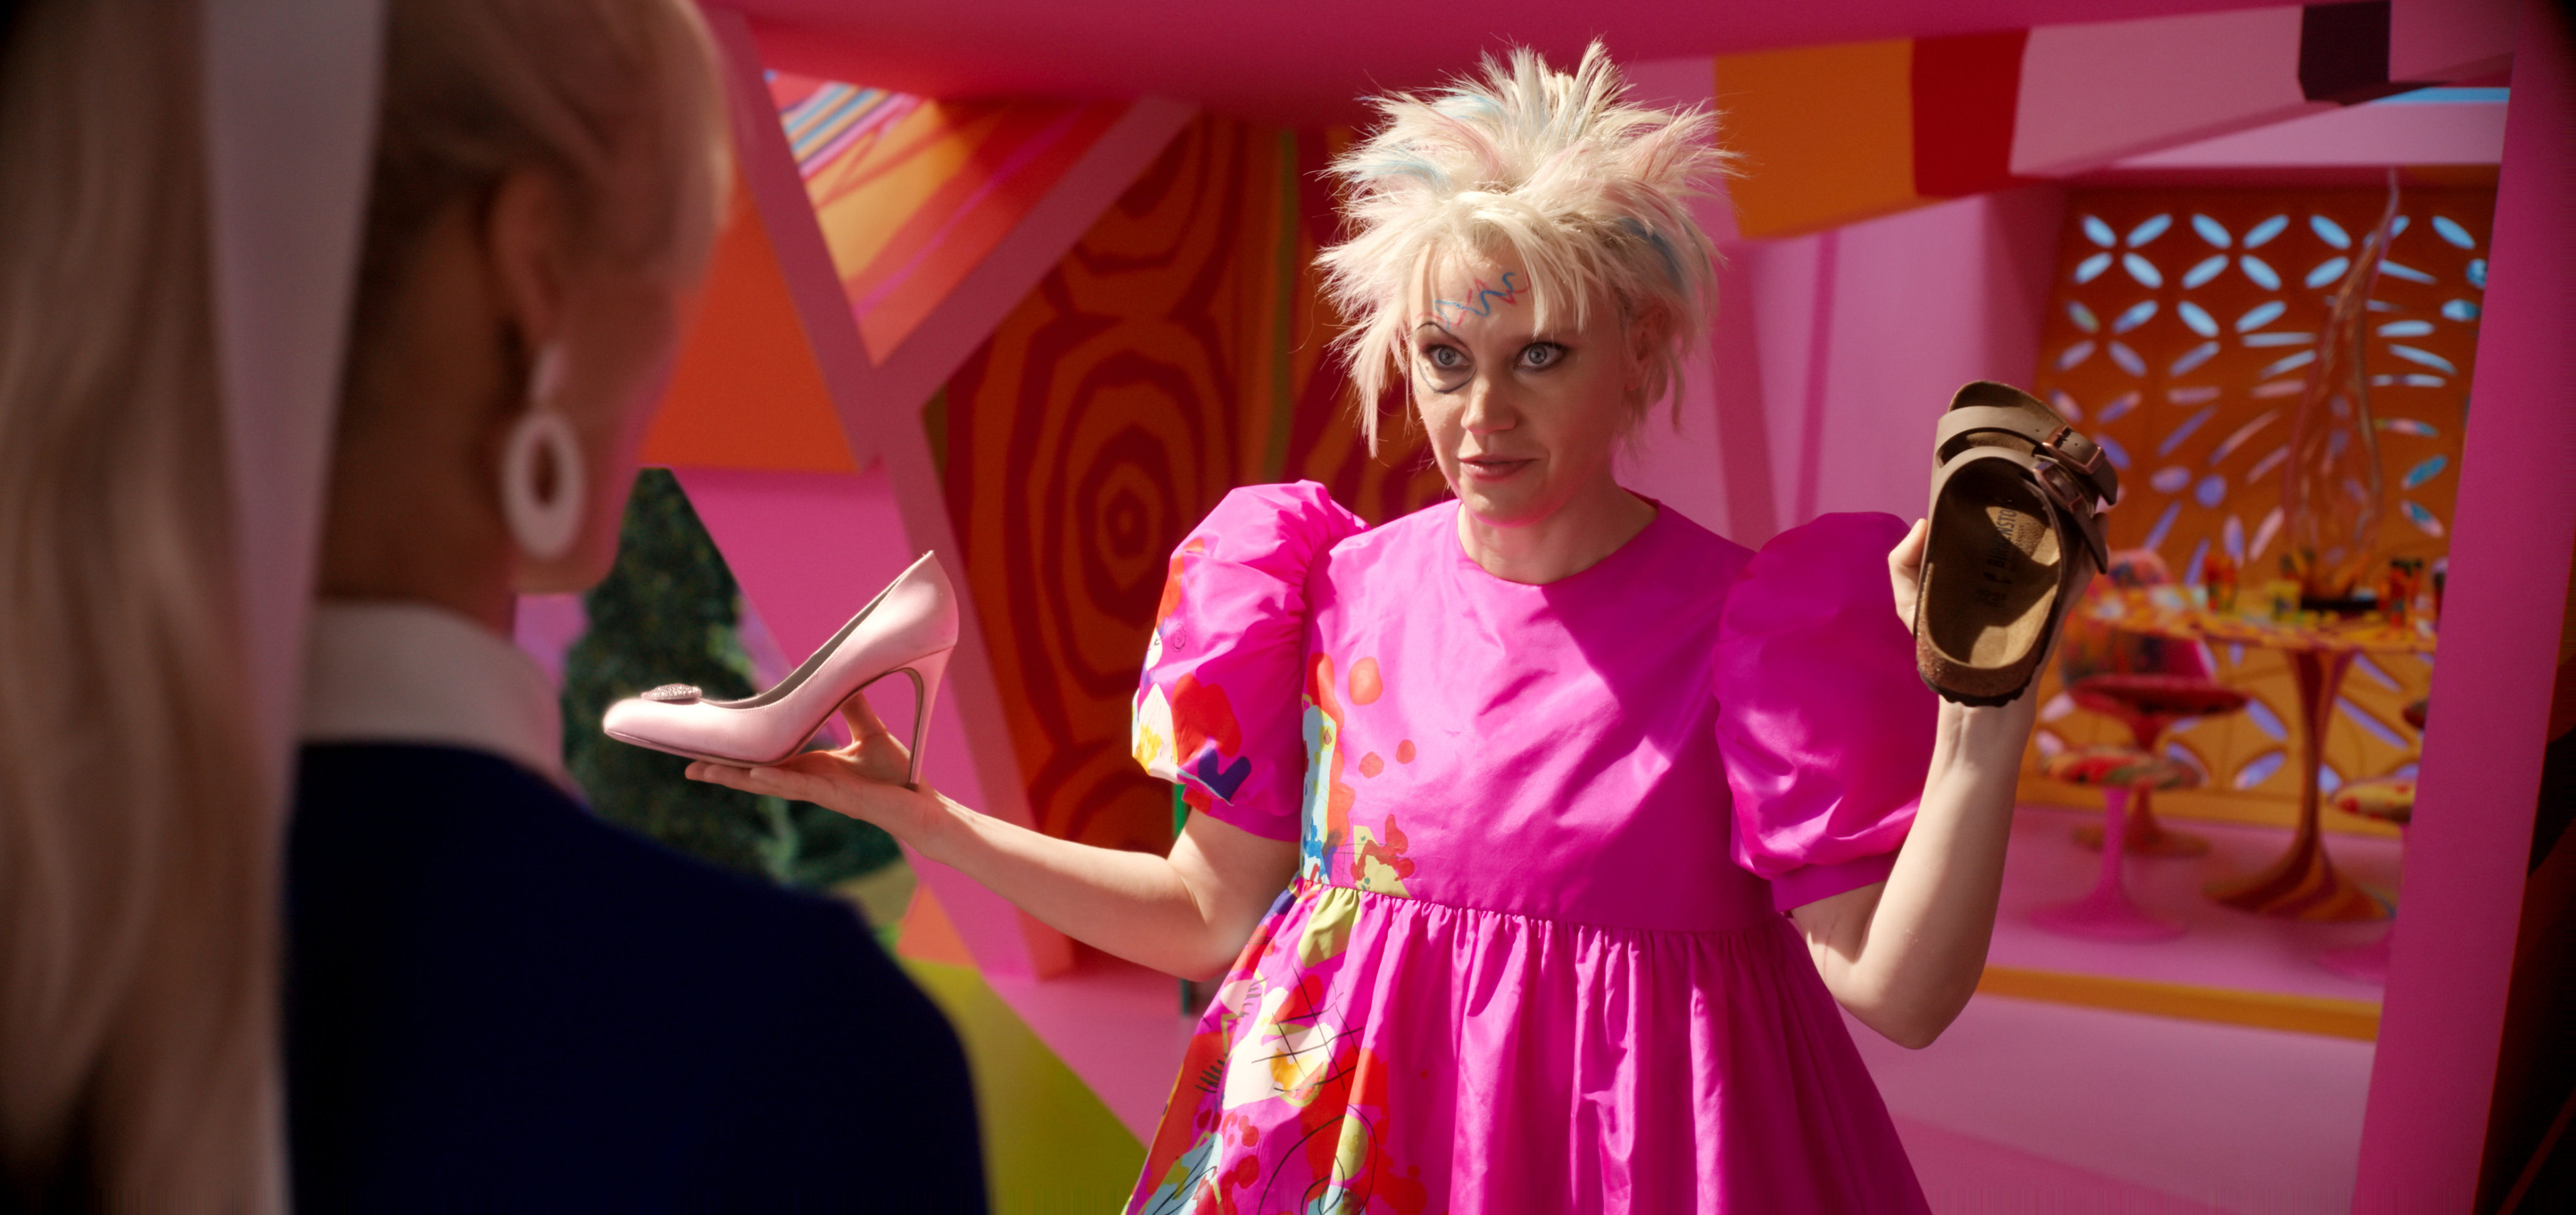
\includegraphics{scripts/01_codingBasics/class2-files/weirdbarbie.jpeg}

}

\caption{photo credit: Warner Bros.}

\end{figure}%

Here's the data below, which you will not (and should not) need to
change:

\begin{Shaded}
\begin{Highlighting}[]
\CommentTok{\# The data {-}{-} DO NOT EDIT }
\NormalTok{ken\_data }\OtherTok{\textless{}{-}} \FunctionTok{data.frame}\NormalTok{(}
  \StringTok{"ken\_name"} \OtherTok{=} \FunctionTok{c}\NormalTok{(}\StringTok{"Ken1"}\NormalTok{, }\StringTok{"Ken2"}\NormalTok{, }\StringTok{"Ken3"}\NormalTok{, }\StringTok{"Ken4"}\NormalTok{, }\StringTok{"Ken5"}\NormalTok{, }\StringTok{"Ken6"}\NormalTok{, }\StringTok{"Ken7"}\NormalTok{, }\StringTok{"Allan"}\NormalTok{),}
  \StringTok{"hair\_color"} \OtherTok{=} \FunctionTok{c}\NormalTok{(}\StringTok{"Blonde"}\NormalTok{, }\StringTok{"Brown"}\NormalTok{, }\StringTok{"Black"}\NormalTok{, }\StringTok{"Red"}\NormalTok{, }\StringTok{"Blonde"}\NormalTok{, }\StringTok{"Brown"}\NormalTok{, }\StringTok{"Black"}\NormalTok{, }\StringTok{"Black"}\NormalTok{),}
  \StringTok{"cowboy\_hats\_owned"} \OtherTok{=} \FunctionTok{c}\NormalTok{(}\DecValTok{2}\NormalTok{, }\DecValTok{0}\NormalTok{, }\DecValTok{1}\NormalTok{, }\DecValTok{3}\NormalTok{, }\DecValTok{0}\NormalTok{, }\DecValTok{1}\NormalTok{, }\DecValTok{2}\NormalTok{, }\DecValTok{0}\NormalTok{),}
  \StringTok{"favorite\_outfit"} \OtherTok{=} \FunctionTok{c}\NormalTok{(}\StringTok{"Casual"}\NormalTok{, }\StringTok{"Formal"}\NormalTok{, }\StringTok{"Sporty"}\NormalTok{, }\StringTok{"Beachwear"}\NormalTok{, }\StringTok{"Formal"}\NormalTok{, }\StringTok{"Casual"}\NormalTok{, }\StringTok{"Sporty"}\NormalTok{, }\StringTok{"Casual"}\NormalTok{),}
  \StringTok{"age"} \OtherTok{=} \FunctionTok{c}\NormalTok{(}\DecValTok{25}\NormalTok{, }\DecValTok{27}\NormalTok{, }\DecValTok{26}\NormalTok{, }\DecValTok{28}\NormalTok{, }\DecValTok{29}\NormalTok{, }\DecValTok{30}\NormalTok{, }\DecValTok{26}\NormalTok{, }\DecValTok{27}\NormalTok{),}
  \StringTok{"height\_cm"} \OtherTok{=} \FunctionTok{c}\NormalTok{(}\DecValTok{180}\NormalTok{, }\DecValTok{175}\NormalTok{, }\DecValTok{182}\NormalTok{, }\DecValTok{178}\NormalTok{, }\DecValTok{180}\NormalTok{, }\DecValTok{183}\NormalTok{, }\DecValTok{177}\NormalTok{, }\DecValTok{175}\NormalTok{),}
  \StringTok{"weight\_kg"} \OtherTok{=} \FunctionTok{c}\NormalTok{(}\DecValTok{75}\NormalTok{, }\DecValTok{70}\NormalTok{, }\DecValTok{80}\NormalTok{, }\DecValTok{77}\NormalTok{, }\DecValTok{76}\NormalTok{, }\DecValTok{78}\NormalTok{, }\DecValTok{79}\NormalTok{, }\DecValTok{70}\NormalTok{),}
  \StringTok{"favorite\_hobby"} \OtherTok{=} \FunctionTok{c}\NormalTok{(}\StringTok{"Surfing"}\NormalTok{, }\StringTok{"Reading"}\NormalTok{, }\StringTok{"Soccer"}\NormalTok{, }\StringTok{"Volleyball"}\NormalTok{, }\StringTok{"Painting"}\NormalTok{, }\StringTok{"Cooking"}\NormalTok{, }\StringTok{"Dancing"}\NormalTok{, }\StringTok{"Guitar"}\NormalTok{),}
  \StringTok{"favorite\_color"} \OtherTok{=} \FunctionTok{c}\NormalTok{(}\StringTok{"Blue"}\NormalTok{, }\StringTok{"Green"}\NormalTok{, }\StringTok{"Red"}\NormalTok{, }\StringTok{"Yellow"}\NormalTok{, }\StringTok{"Purple"}\NormalTok{, }\StringTok{"Orange"}\NormalTok{, }\StringTok{"Pink"}\NormalTok{, }\StringTok{"Blue"}\NormalTok{),}
  \StringTok{"shoe\_size"} \OtherTok{=} \FunctionTok{c}\NormalTok{(}\DecValTok{10}\NormalTok{, }\DecValTok{9}\NormalTok{, }\DecValTok{11}\NormalTok{, }\DecValTok{10}\NormalTok{, }\ConstantTok{NA}\NormalTok{, }\DecValTok{11}\NormalTok{, }\DecValTok{10}\NormalTok{, }\DecValTok{9}\NormalTok{),}
  \StringTok{"best\_friend"} \OtherTok{=} \FunctionTok{c}\NormalTok{(}\StringTok{"Barbie"}\NormalTok{, }\StringTok{"Barbie"}\NormalTok{, }\StringTok{"Barbie"}\NormalTok{, }\StringTok{"Barbie"}\NormalTok{, }\StringTok{"Barbie"}\NormalTok{, }\StringTok{"Barbie"}\NormalTok{, }\StringTok{"Barbie"}\NormalTok{, }\ConstantTok{NA}\NormalTok{),}
  \StringTok{"is\_ken"} \OtherTok{=} \FunctionTok{c}\NormalTok{(}\ConstantTok{TRUE}\NormalTok{, }\ConstantTok{TRUE}\NormalTok{, }\ConstantTok{TRUE}\NormalTok{, }\ConstantTok{TRUE}\NormalTok{, }\ConstantTok{TRUE}\NormalTok{, }\ConstantTok{TRUE}\NormalTok{, }\ConstantTok{TRUE}\NormalTok{, }\ConstantTok{FALSE}\NormalTok{)}
\NormalTok{)}
\end{Highlighting}
\end{Shaded}

However, as is typical of Weird Barbie, her code is\ldots weird. In
almost all other aspects of life, that's OK! But when it comes to you,
three years later, trying to figure out what she did\ldots not ideal.
Here's her code below. As it's written, there are many bugs (code errors
that either return an error or return an unexpected/incorrect result),
the style is inconsistent, and there is no documentation. Using what you
have learned so far, fix Weird Barbie's code: find the bugs, smash the
bugs (get the code to run), change to a consistent style, and add
helpful comments. You may need to consult the style guide mentioned in
Class 0, help pages, and Google.

\begin{Shaded}
\begin{Highlighting}[]
\FunctionTok{str}\NormalTok{(ken\_data)}
\FunctionTok{haed}\NormalTok{(ken\_data)}

\FunctionTok{mean}\NormalTok{(ken\_data}\SpecialCharTok{$}\NormalTok{cowboy\_hats\_owned)}
\FunctionTok{hist}\NormalTok{(ken\_data}\SpecialCharTok{$}\NormalTok{cowboy\_hats\_owned)}
\NormalTok{ken\_data}\SpecialCharTok{$}\NormalTok{more.than}\FloatTok{.1}\NormalTok{\_cowboyHat }\OtherTok{\textless{}{-}}\NormalTok{ ken\_data}\SpecialCharTok{$}\NormalTok{cowboy\_hats\_owned }\SpecialCharTok{\textgreater{}} \DecValTok{1}
\FunctionTok{print}\NormalTok{(}\FunctionTok{paste}\NormalTok{(}\FunctionTok{sum}\NormalTok{(ken\_data}\SpecialCharTok{$}\NormalTok{more.than}\FloatTok{.1}\NormalTok{\_cowboyHat), }\StringTok{"Kens have more than 1 cowboy hat"}\NormalTok{))}

\FunctionTok{range}\NormalTok{(ken}\SpecialCharTok{$}\NormalTok{age)}
\FunctionTok{range}\NormalTok{(ken\_data}\SpecialCharTok{$}\NormalTok{shoe\_size)}


\NormalTok{correlation }\OtherTok{\textless{}{-}} \FunctionTok{cor}\NormalTok{(ken\_data}\SpecialCharTok{$}\NormalTok{height\_cm, ken\_data}\SpecialCharTok{$}\NormalTok{weight\_kg)}
\FunctionTok{print}\NormalTok{(}\FunctionTok{paste}\NormalTok{(}\StringTok{"The correlation between height and weight is"}\NormalTok{, correlation))}
\FunctionTok{plot}\NormalTok{(ken\_data}\SpecialCharTok{$}\NormalTok{height\_cm, ken\_data}\SpecialCharTok{$}\NormalTok{weight\_kg)}

\FunctionTok{table}\NormalTok{(ken\_data}\SpecialCharTok{$}\NormalTok{best\_friend)}
\CommentTok{\# looks like everyone\textquotesingle{}s bff is barbie!}

\CommentTok{\# outfits}
\FunctionTok{table}\NormalTok{(ken\_data}\SpecialCharTok{$}\NormalTok{favorte\_outfit)}


\CommentTok{\# no allan}
\FunctionTok{range}\NormalTok{(ken\_data[}\DecValTok{1}\SpecialCharTok{:}\DecValTok{7}\NormalTok{,}\DecValTok{5}\NormalTok{])}

\NormalTok{noAllan }\OtherTok{\textless{}{-}}\NormalTok{ ken\_data[}\DecValTok{1}\SpecialCharTok{:}\DecValTok{7}\NormalTok{,]}
\NormalTok{also\_noAllan }\OtherTok{\textless{}{-}}\NormalTok{ noAllan }\OtherTok{\textless{}{-}}\NormalTok{ ken\_data[ken\_data}\SpecialCharTok{$}\NormalTok{is\_ken }\SpecialCharTok{==} \ConstantTok{TRUE}\NormalTok{,]}
\FunctionTok{range}\NormalTok{(noAllan}\SpecialCharTok{$}\NormalTok{shoe\_size)}

\CommentTok{\# Are the sporty Kens taller than the other Kens?}
\NormalTok{sporty\_kens }\OtherTok{\textless{}{-}} \FunctionTok{mean}\NormalTok{( ken\_data [ken\_data}\SpecialCharTok{$}\NormalTok{favorite\_outfit }\SpecialCharTok{==} \StringTok{"Sporty"}\NormalTok{, }\StringTok{"height\_cm"}\NormalTok{])}
\NormalTok{other\_kens\_mean }\OtherTok{\textless{}{-}} \FunctionTok{mean}\NormalTok{(ken\_data[ken\_data}\SpecialCharTok{$}\NormalTok{favorite\_outfit }\SpecialCharTok{!=} \StringTok{"Sporty"}\NormalTok{, }\StringTok{"height\_cm"}\NormalTok{] )}

\NormalTok{sporty\_kens }\SpecialCharTok{\textgreater{}}\NormalTok{ other\_kens\_mean}
\end{Highlighting}
\end{Shaded}

\bookmarksetup{startatroot}

\chapter{Let's Get Plotting!}\label{lets-get-plotting}

Data Visualization, Day 1

\hfill\break

For this lesson, we will be using a .bed file of genetic variants from
\url{https://marianattestad.com/blog}. We will need to read in this data
using the \texttt{read.table()} function, then rename the columns with
the \texttt{name()} function:

\begin{Shaded}
\begin{Highlighting}[]
\NormalTok{variants }\OtherTok{\textless{}{-}} \FunctionTok{read.table}\NormalTok{(}\StringTok{"DataVizDay1{-}files/variants\_from\_assembly.bed"}\NormalTok{, }\AttributeTok{sep=}\StringTok{"}\SpecialCharTok{\textbackslash{}t}\StringTok{"}\NormalTok{, }\AttributeTok{quote=}\StringTok{\textquotesingle{}\textquotesingle{}}\NormalTok{, }\AttributeTok{stringsAsFactors=}\ConstantTok{TRUE}\NormalTok{,}\AttributeTok{header=}\ConstantTok{FALSE}\NormalTok{)}
\FunctionTok{names}\NormalTok{(variants) }\OtherTok{\textless{}{-}} \FunctionTok{c}\NormalTok{(}\StringTok{"chrom"}\NormalTok{,}\StringTok{"start"}\NormalTok{,}\StringTok{"stop"}\NormalTok{,}\StringTok{"name"}\NormalTok{,}\StringTok{"size"}\NormalTok{,}\StringTok{"strand"}\NormalTok{,}\StringTok{"type"}\NormalTok{,}\StringTok{"ref.dist"}\NormalTok{,}\StringTok{"query.dist"}\NormalTok{)}
\end{Highlighting}
\end{Shaded}

Let's take a look at this dataset and what kind of research questions we
could explore using this data.

\begin{Shaded}
\begin{Highlighting}[]
\FunctionTok{head}\NormalTok{(variants)}
\end{Highlighting}
\end{Shaded}

\begin{verbatim}
  chrom     start      stop name size strand      type ref.dist query.dist
1     6 103832058 103832059  SV1  185      + Insertion        0        185
2     6 102958468 102958469  SV2  317      + Insertion      -14        303
3     6 102741692 102741693  SV3  130      +  Deletion      130          0
4     6 102283759 102283760  SV4 1271      + Insertion      -12       1259
5     6 101194032 101194033  SV5 2864      + Insertion      -13       2851
6     6 101056644 101056645  SV6  265      + Insertion        0        265
\end{verbatim}

There are 9 different columns in this dataset, the genomic position
(chrom, start, stop), name, size, strand, distance to reference
(ref.dist) and distance to query (query.dist). What are some questions
we could ask about this data?

Some examples:

\begin{itemize}
\item
  What is the distribution of distances to the reference?
\item
  Are the sizes of variants of different types different?
\end{itemize}

We can quickly explore questions like these by creating quick
visualizations of the data.

\section{Let's Get Plotting!}\label{lets-get-plotting-1}

\textbf{Choosing a plot type}

Data visualizations can tell us about the relationships of different
variables in a data set. There are 3 main categories of these
relationships, each answering a different type of question about the
data.

\begin{enumerate}
\def\labelenumi{\arabic{enumi}.}
\tightlist
\item
  The variation \emph{within} a single variable

  \begin{itemize}
  \tightlist
  \item
    How do expression levels of a gene vary among patient samples?
  \end{itemize}
\item
  The co-variation \emph{between} a continuous and categorical variable

  \begin{itemize}
  \tightlist
  \item
    How does beak size compare between penguins living on different
    islands?
  \end{itemize}
\item
  The co-variation \emph{between} two continuous variables

  \begin{itemize}
  \tightlist
  \item
    How does trunk thickness relate to the age of a tree?
  \end{itemize}
\end{enumerate}

\begin{tcolorbox}[enhanced jigsaw, bottomtitle=1mm, bottomrule=.15mm, toprule=.15mm, opacityback=0, leftrule=.75mm, breakable, colback=white, toptitle=1mm, left=2mm, coltitle=black, titlerule=0mm, opacitybacktitle=0.6, title=\textcolor{quarto-callout-tip-color}{\faLightbulb}\hspace{0.5em}{Tip \ref*{tip-example}: Differentiating between continuous variables and categorical variables
that are represented by a number}, rightrule=.15mm, arc=.35mm, colframe=quarto-callout-tip-color-frame, colbacktitle=quarto-callout-tip-color!10!white]

\quartocallouttip{tip-example} 

\begin{itemize}
\tightlist
\item
  If you can replace the number with a descriptor and it still makes
  sense, it is a categorical variable

  \begin{itemize}
  \tightlist
  \item
    you can tell R that this is a categorical variable by using
    \texttt{factor()} or \texttt{character()}
  \end{itemize}
\end{itemize}

i.e.~chromosome 1 and chromosome 2 could be re-labeled as chromosome A
and chromosome B or ``first chromosome'' and ``second chromosome''
without fundamentally changing the information

\begin{itemize}
\tightlist
\item
  If you can add/subtract two values and it still makes sense, it is a
  continuous variable
\end{itemize}

i.e.~subtracting chromosome 6 - 2 = 4, this 4 doesn't mean anything, but
subtracting size 317 - 185 = 132, this means one variant is 132 bp
larger than the other

\end{tcolorbox}

There are 2 main ways we create plots in R

\begin{enumerate}
\def\labelenumi{\arabic{enumi}.}
\item
  Using base R functions (i.e.~\texttt{plot()})
\item
  Using tidyverse functions (i.e.~\texttt{ggplot()})

  \begin{itemize}
  \tightlist
  \item
    This requires loading the \texttt{ggplot2} package with
    \texttt{library(ggplot2)}
  \end{itemize}
\end{enumerate}

\subsection{Numeric vs Numeric}\label{numeric-vs-numeric}

Let's try this with a plot type you are likely very familiar with: a
scatterplot

A scatterplot looks at co-variation between 2 numeric variables, so what
are 2 numeric variables we have in this dataset?

Let's try plotting \texttt{ref.dist} vs \texttt{query.dist}:

\subsubsection{Base R}\label{base-r}

For base R, the \texttt{plot()} function takes in vectors of x and y
values to plot.

Q: How do we extract the entire column of \texttt{ref.dist} and
\texttt{query.dist} from our dataset, \texttt{variants}?

A: \texttt{variants\$ref.dist} and \texttt{variants\$query.dist}

\begin{Shaded}
\begin{Highlighting}[]
\DocumentationTok{\#\# create a scatterplot}
\FunctionTok{plot}\NormalTok{(}\AttributeTok{x =}\NormalTok{ variants}\SpecialCharTok{$}\NormalTok{ref.dist, }\AttributeTok{y =}\NormalTok{ variants}\SpecialCharTok{$}\NormalTok{query.dist)}
\end{Highlighting}
\end{Shaded}

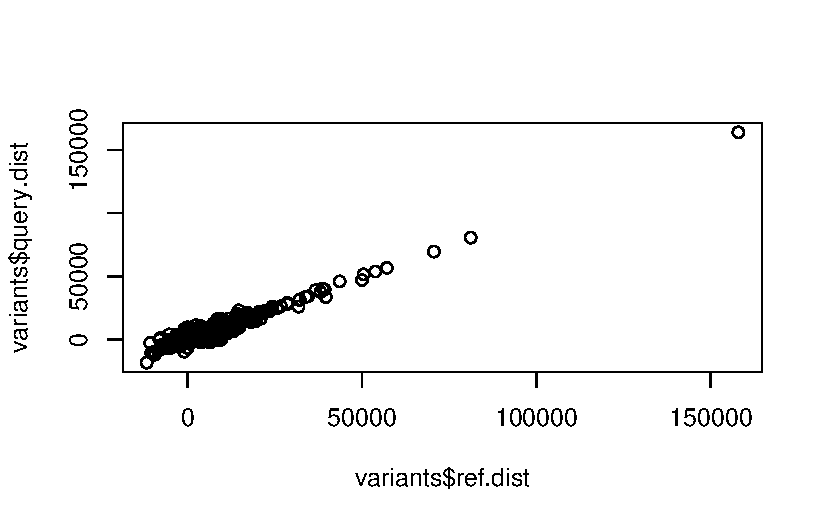
\includegraphics{scripts/02_dataViz/class3_files/figure-pdf/unnamed-chunk-3-1.pdf}

That's great! But it's not easy to understand what these x and y axes
are, so let's relabel them by changing the parameters \texttt{xlab} and
\texttt{ylab} inside the \texttt{plot()} function call

\begin{Shaded}
\begin{Highlighting}[]
\DocumentationTok{\#\# create a scatterplot with better axes labels}
\FunctionTok{plot}\NormalTok{(}\AttributeTok{x =}\NormalTok{ variants}\SpecialCharTok{$}\NormalTok{ref.dist, }\AttributeTok{y =}\NormalTok{ variants}\SpecialCharTok{$}\NormalTok{query.dist,}
     \AttributeTok{xlab =} \StringTok{"Reference distance"}\NormalTok{, }\AttributeTok{ylab =} \StringTok{"Query Distance"}\NormalTok{)}
\end{Highlighting}
\end{Shaded}

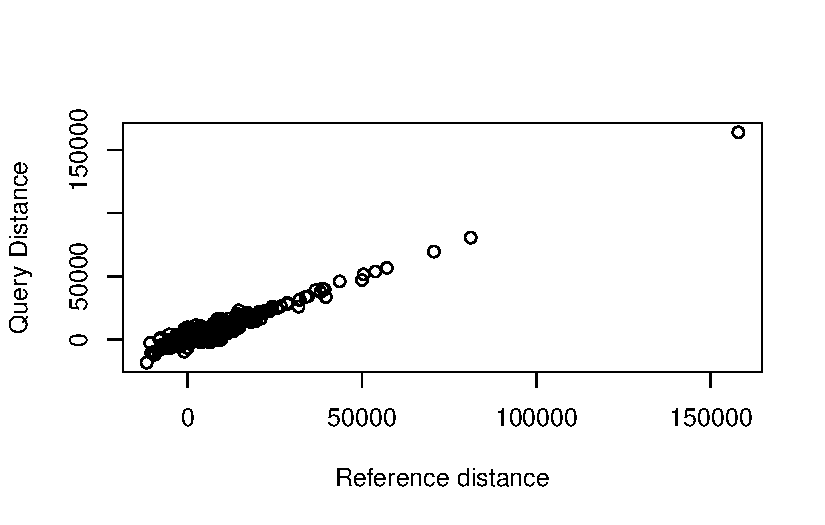
\includegraphics{scripts/02_dataViz/class3_files/figure-pdf/unnamed-chunk-4-1.pdf}

Great! We can also add a title and subtitle with \texttt{main} and
\texttt{sub}, try this on your own!

Other plot types:

\begin{longtable}[]{@{}ll@{}}
\toprule\noalign{}
Function & Plot Type \\
\midrule\noalign{}
\endhead
\bottomrule\noalign{}
\endlastfoot
\texttt{plot()} & scatterplot \\
\texttt{lines()} or \texttt{plot(type\ =\ "l")} & line plot \\
\end{longtable}

To plot a line on top of points, you can run \texttt{lines()} with the
same data immediately following \texttt{plot()}. Notice that the line
connects \emph{all} points, leading to a bit of a jumbled mess. How do
you think we can fix this?

\begin{Shaded}
\begin{Highlighting}[]
\DocumentationTok{\#\# line plot}
\FunctionTok{plot}\NormalTok{(}\AttributeTok{x =}\NormalTok{ variants}\SpecialCharTok{$}\NormalTok{ref.dist, }\AttributeTok{y =}\NormalTok{ variants}\SpecialCharTok{$}\NormalTok{query.dist,}
     \AttributeTok{xlab =} \StringTok{"Reference distance"}\NormalTok{, }\AttributeTok{ylab =} \StringTok{"Query Distance"}\NormalTok{)}
\FunctionTok{lines}\NormalTok{(}\AttributeTok{x =}\NormalTok{ variants}\SpecialCharTok{$}\NormalTok{ref.dist, }\AttributeTok{y =}\NormalTok{ variants}\SpecialCharTok{$}\NormalTok{query.dist)}
\end{Highlighting}
\end{Shaded}

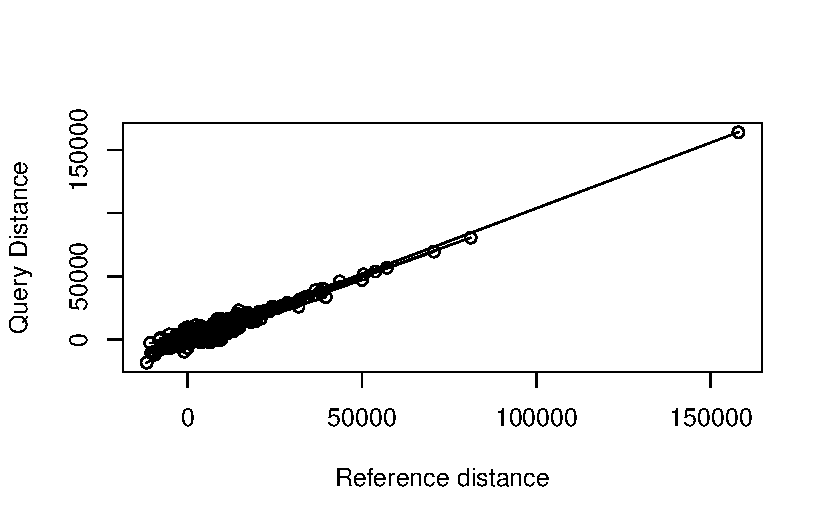
\includegraphics{scripts/02_dataViz/class3_files/figure-pdf/unnamed-chunk-5-1.pdf}

\subsubsection{ggplot}\label{ggplot}

For more complex layered plots, we can also use \texttt{ggplot()} from
the \texttt{ggplot2} package. ``gg'' stands for ``grammar of graphics''
and plots are built a bit like sentences with different parts building
on each other.

To start, let's load in the \texttt{ggplot2} package. You will only need
to do this once.

\begin{Shaded}
\begin{Highlighting}[]
\DocumentationTok{\#\# load the ggplot2 library}
\FunctionTok{library}\NormalTok{(ggplot2)}
\end{Highlighting}
\end{Shaded}

Now each time we want to make a plot, you will start by using
\texttt{ggplot()}.

\begin{Shaded}
\begin{Highlighting}[]
\FunctionTok{ggplot}\NormalTok{()}
\end{Highlighting}
\end{Shaded}


\includegraphics{scripts/02_dataViz/class3_files/figure-pdf/unnamed-chunk-7-1.pdf}

We haven't given this function any data, so right now we just have an
empty grey box.

The first layer we can add is the data. \texttt{ggplot()} requires the
name of the dataset once, then you can just use column names throughout
the rest of the code instead of using \texttt{dataset\$var1},
\texttt{dataset\$var2}, \texttt{dataset\$var3} , etc.

\begin{Shaded}
\begin{Highlighting}[]
\FunctionTok{ggplot}\NormalTok{(variants)}
\end{Highlighting}
\end{Shaded}


\includegraphics{scripts/02_dataViz/class3_files/figure-pdf/unnamed-chunk-8-1.pdf}

We still have a grey box! Although we have told the function we want to
use data from the \texttt{variants} dataset, we didn't tell it
\emph{which} data we want to use. Any time you are referencing a column
name to set the position, color, size, etc. of a point, you need to wrap
it inside \texttt{aes()}, which is short for ``aesthetics''. This looks
something like this:

\begin{Shaded}
\begin{Highlighting}[]
\FunctionTok{ggplot}\NormalTok{(variants, }\FunctionTok{aes}\NormalTok{(}\AttributeTok{x =}\NormalTok{ ref.dist, }\AttributeTok{y =}\NormalTok{ query.dist))}
\end{Highlighting}
\end{Shaded}

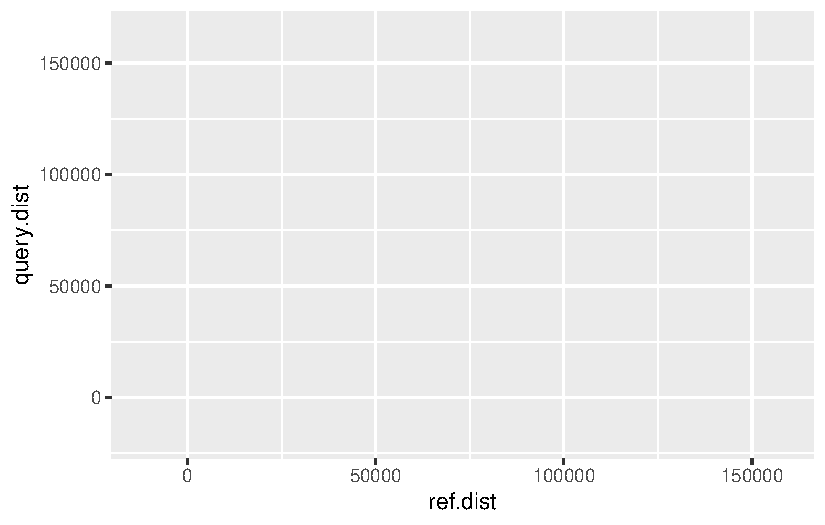
\includegraphics{scripts/02_dataViz/class3_files/figure-pdf/unnamed-chunk-9-1.pdf}

More than a grey box! Now that we know which variables we are plotting
and the dataset they come from, we have the framework to add the next
layer: geometry. The geometry, as you might guess, refers to what type
of shapes to put on the plot. Is it a line? A point? A bar? For
scatterplots, we want the data represented as points, so we will use
\texttt{geom\_point()}.

Whenever we add a \texttt{ggplot} layer, we will connect it to the
current plot using a \texttt{+} sign:

\begin{Shaded}
\begin{Highlighting}[]
\FunctionTok{ggplot}\NormalTok{(variants, }\FunctionTok{aes}\NormalTok{(}\AttributeTok{x =}\NormalTok{ ref.dist, }\AttributeTok{y =}\NormalTok{ query.dist)) }\SpecialCharTok{+}
  \FunctionTok{geom\_point}\NormalTok{() }\CommentTok{\# plot as points}
\end{Highlighting}
\end{Shaded}

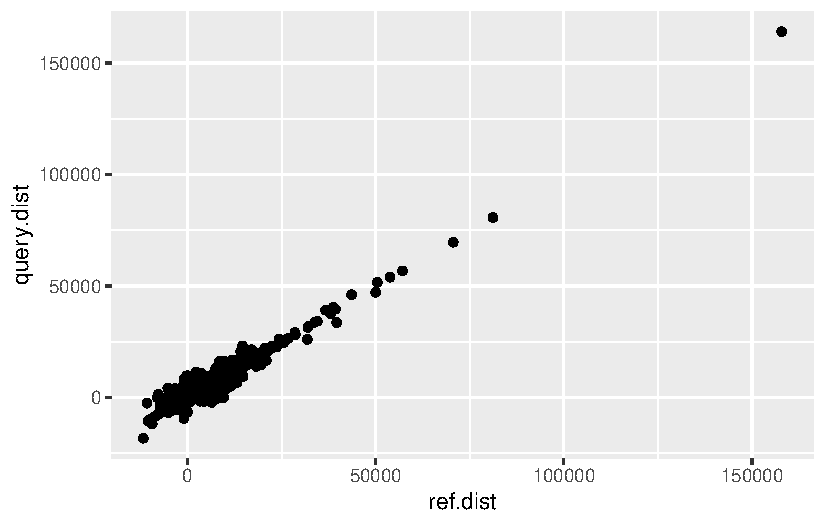
\includegraphics{scripts/02_dataViz/class3_files/figure-pdf/unnamed-chunk-10-1.pdf}

Voila! We have our scatterplot! Now we can continue adding layers to
change things like the labels. Use the \texttt{labs()} function to
change the x, y, and optionally the title and subtitle:

\begin{Shaded}
\begin{Highlighting}[]
\FunctionTok{ggplot}\NormalTok{(variants, }\FunctionTok{aes}\NormalTok{(}\AttributeTok{x =}\NormalTok{ ref.dist, }\AttributeTok{y =}\NormalTok{ query.dist)) }\SpecialCharTok{+}
  \FunctionTok{geom\_point}\NormalTok{() }\SpecialCharTok{+} \CommentTok{\# plot as points}
  \FunctionTok{labs}\NormalTok{(}\AttributeTok{x =} \StringTok{"Reference Distance"}\NormalTok{,}
       \AttributeTok{y =} \StringTok{"Query Distance"}\NormalTok{,}
       \AttributeTok{title =} \StringTok{"Plot Title"}\NormalTok{,}
       \AttributeTok{subtitle =} \StringTok{"Plot Subtitle"}\NormalTok{)}
\end{Highlighting}
\end{Shaded}

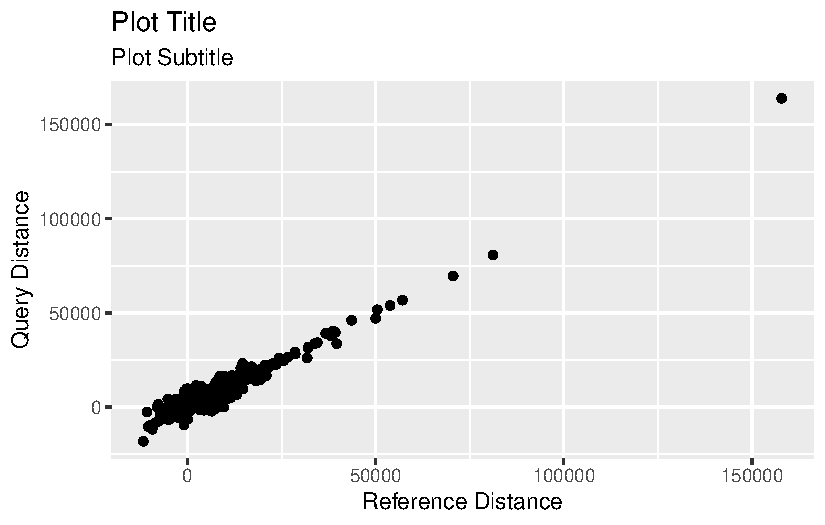
\includegraphics{scripts/02_dataViz/class3_files/figure-pdf/unnamed-chunk-11-1.pdf}

ggplots will all follow this general formula, changing the \texttt{geom}
for different plot types.

Other plot types:

\begin{longtable}[]{@{}ll@{}}
\toprule\noalign{}
Function & Plot Type \\
\midrule\noalign{}
\endhead
\bottomrule\noalign{}
\endlastfoot
\texttt{geom\_point()} & scatterplot \\
\texttt{geom\_line()} & line plot \\
\texttt{geom\_smooth()} & line plot of smoothed averages \\
\end{longtable}

To plot a line on top of points, you can add a second geom, using
\texttt{geom\_point()} + \texttt{geom\_line()}.

\begin{Shaded}
\begin{Highlighting}[]
\FunctionTok{ggplot}\NormalTok{(variants, }\FunctionTok{aes}\NormalTok{(}\AttributeTok{x =}\NormalTok{ ref.dist, }\AttributeTok{y =}\NormalTok{ query.dist)) }\SpecialCharTok{+}
  \FunctionTok{geom\_point}\NormalTok{() }\SpecialCharTok{+} \CommentTok{\# plot as points}
  \FunctionTok{geom\_line}\NormalTok{() }\SpecialCharTok{+} \CommentTok{\# plot as line}
  \FunctionTok{labs}\NormalTok{(}\AttributeTok{x =} \StringTok{"Reference Distance"}\NormalTok{,}
       \AttributeTok{y =} \StringTok{"Query Distance"}\NormalTok{,}
       \AttributeTok{title =} \StringTok{"Plot Title"}\NormalTok{,}
       \AttributeTok{subtitle =} \StringTok{"Plot Subtitle"}\NormalTok{)}
\end{Highlighting}
\end{Shaded}

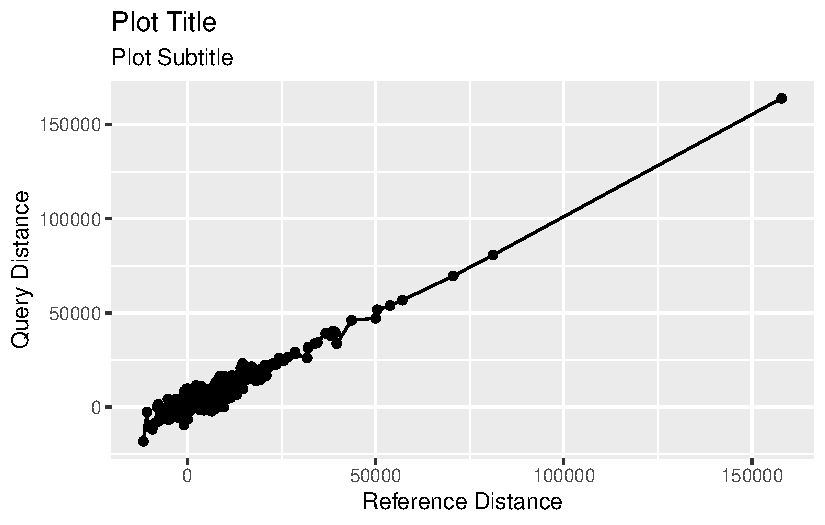
\includegraphics{scripts/02_dataViz/class3_files/figure-pdf/unnamed-chunk-12-1.pdf}

\begin{Shaded}
\begin{Highlighting}[]
\FunctionTok{ggplot}\NormalTok{(variants, }\FunctionTok{aes}\NormalTok{(}\AttributeTok{x =}\NormalTok{ ref.dist, }\AttributeTok{y =}\NormalTok{ query.dist)) }\SpecialCharTok{+}
  \FunctionTok{geom\_smooth}\NormalTok{() }\SpecialCharTok{+} \CommentTok{\# plot as smooth line}
  \FunctionTok{labs}\NormalTok{(}\AttributeTok{x =} \StringTok{"Reference Distance"}\NormalTok{,}
       \AttributeTok{y =} \StringTok{"Query Distance"}\NormalTok{,}
       \AttributeTok{title =} \StringTok{"Plot Title"}\NormalTok{,}
       \AttributeTok{subtitle =} \StringTok{"Plot Subtitle"}\NormalTok{)}
\end{Highlighting}
\end{Shaded}

\begin{verbatim}
`geom_smooth()` using method = 'gam' and formula = 'y ~ s(x, bs = "cs")'
\end{verbatim}

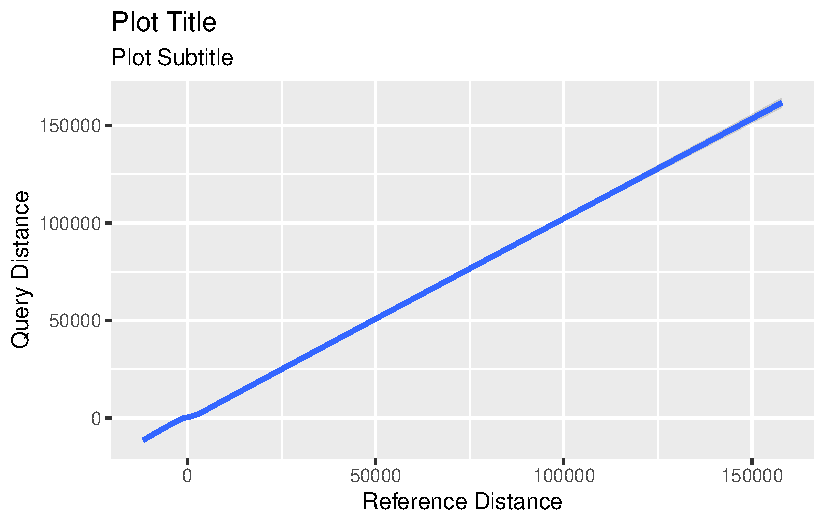
\includegraphics{scripts/02_dataViz/class3_files/figure-pdf/unnamed-chunk-12-2.pdf}

\subsection{Numeric Distribution}\label{numeric-distribution}

Sometimes we want to look at the distribution or spread of values for
one continuous variable. For example, in our data, what is the
distribution of sizes for our variants?

There are several plot types we can use to explore this question

\begin{longtable}[]{@{}lll@{}}
\toprule\noalign{}
Plot Type & Base R Function & ggplot Function \\
\midrule\noalign{}
\endhead
\bottomrule\noalign{}
\endlastfoot
histogram & \texttt{hist()} & \texttt{geom\_histogram()} \\
density plot & \texttt{plot(density())} & \texttt{geom\_density()} \\
boxplot & \texttt{boxplot()} & \texttt{geom\_boxplot()} \\
violin plot & not available & \texttt{geom\_violin()} \\
bar plot & \texttt{barplot(table())} &
\texttt{geom\_bar(stat\ =\ "identity")} \\
\end{longtable}

\begin{tcolorbox}[enhanced jigsaw, bottomtitle=1mm, bottomrule=.15mm, toprule=.15mm, opacityback=0, leftrule=.75mm, breakable, colback=white, toptitle=1mm, left=2mm, coltitle=black, titlerule=0mm, opacitybacktitle=0.6, title=\textcolor{quarto-callout-tip-color}{\faLightbulb}\hspace{0.5em}{Tip}, rightrule=.15mm, arc=.35mm, colframe=quarto-callout-tip-color-frame, colbacktitle=quarto-callout-tip-color!10!white]

Try \texttt{?function\_name()} to learn more about the different
parameters used to customize each function

\end{tcolorbox}

\subsubsection{Base R}\label{base-r-1}

In base R, we can pass each plotting function the vector of values that
we want to plot. In this case, we want to plot all of the values in the
\texttt{size} column of \texttt{variants}, so we will pass in
\texttt{variants\$size} to our plotting functions.

\begin{Shaded}
\begin{Highlighting}[]
\DocumentationTok{\#\# histogram}
\FunctionTok{hist}\NormalTok{(variants}\SpecialCharTok{$}\NormalTok{size)}
\end{Highlighting}
\end{Shaded}

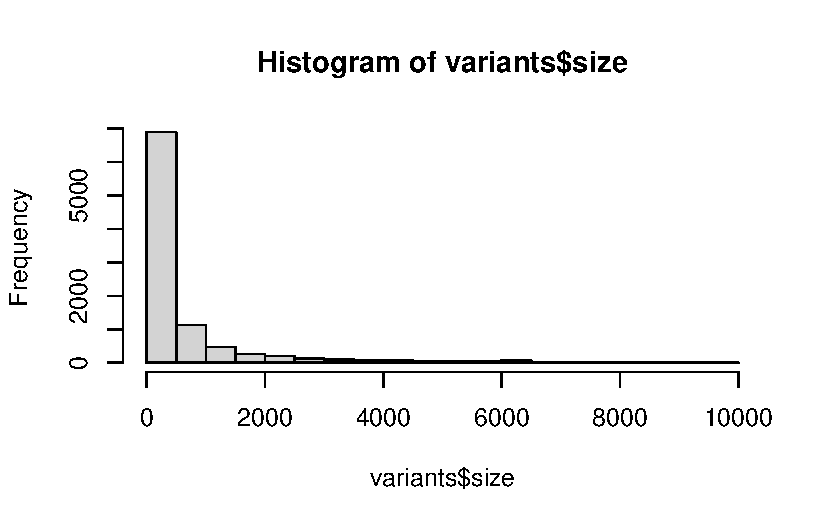
\includegraphics{scripts/02_dataViz/class3_files/figure-pdf/unnamed-chunk-13-1.pdf}

\begin{Shaded}
\begin{Highlighting}[]
\DocumentationTok{\#\# density plot}
\FunctionTok{plot}\NormalTok{(}\FunctionTok{density}\NormalTok{(variants}\SpecialCharTok{$}\NormalTok{size))}
\end{Highlighting}
\end{Shaded}

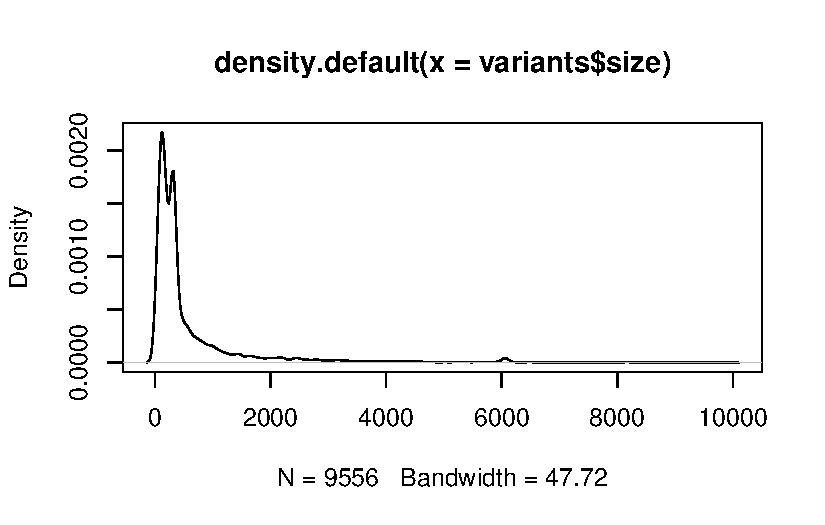
\includegraphics{scripts/02_dataViz/class3_files/figure-pdf/unnamed-chunk-13-2.pdf}

\begin{Shaded}
\begin{Highlighting}[]
\DocumentationTok{\#\# boxplot}
\FunctionTok{boxplot}\NormalTok{(variants}\SpecialCharTok{$}\NormalTok{size)}
\end{Highlighting}
\end{Shaded}

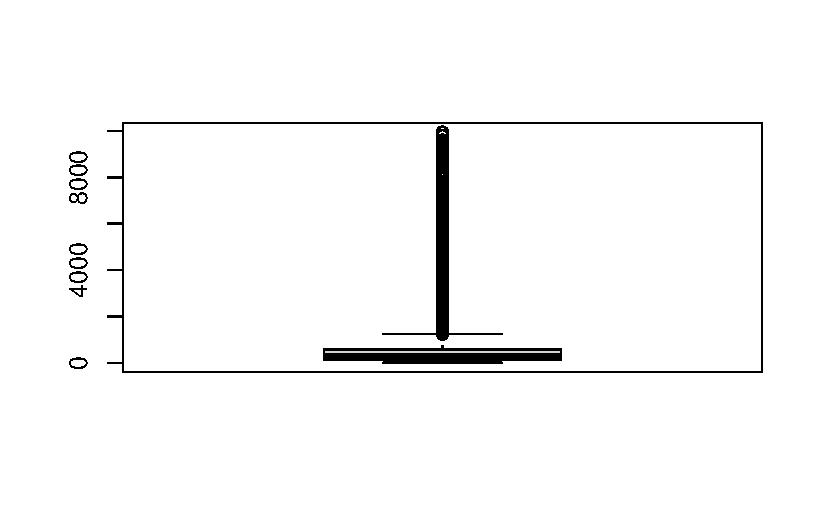
\includegraphics{scripts/02_dataViz/class3_files/figure-pdf/unnamed-chunk-13-3.pdf}

Try adding labels and titles as described before.

\subsubsection{ggplot}\label{ggplot-1}

In ggplot, we start by calling the base \texttt{ggplot()} function with
the entire dataset, \texttt{variants}, then we can set the aesthetics of
the x value to our column of interest with \texttt{aes(x\ =\ size)}.
Then, we can add unique geoms for each plot type.

\begin{Shaded}
\begin{Highlighting}[]
\DocumentationTok{\#\# histogram}
\FunctionTok{ggplot}\NormalTok{(variants, }\FunctionTok{aes}\NormalTok{(}\AttributeTok{x =}\NormalTok{ size)) }\SpecialCharTok{+}
  \FunctionTok{geom\_histogram}\NormalTok{()}
\end{Highlighting}
\end{Shaded}

\begin{verbatim}
`stat_bin()` using `bins = 30`. Pick better value with `binwidth`.
\end{verbatim}

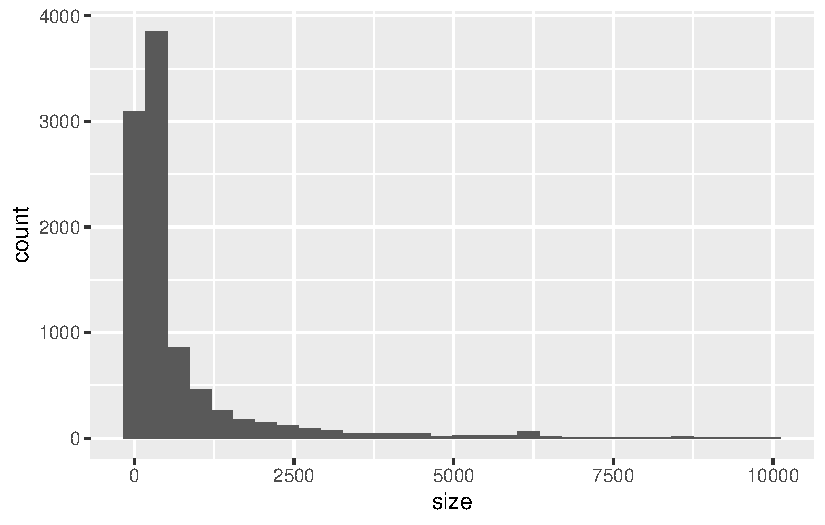
\includegraphics{scripts/02_dataViz/class3_files/figure-pdf/unnamed-chunk-14-1.pdf}

\begin{Shaded}
\begin{Highlighting}[]
\DocumentationTok{\#\# density}
\FunctionTok{ggplot}\NormalTok{(variants, }\FunctionTok{aes}\NormalTok{(}\AttributeTok{x =}\NormalTok{ size)) }\SpecialCharTok{+}
  \FunctionTok{geom\_density}\NormalTok{()}
\end{Highlighting}
\end{Shaded}

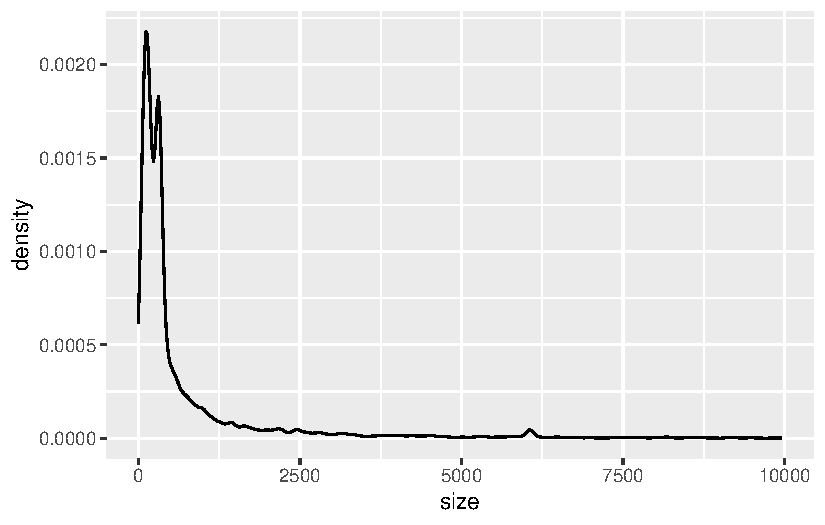
\includegraphics{scripts/02_dataViz/class3_files/figure-pdf/unnamed-chunk-14-2.pdf}

\begin{Shaded}
\begin{Highlighting}[]
\DocumentationTok{\#\# boxplot}
\FunctionTok{ggplot}\NormalTok{(variants, }\FunctionTok{aes}\NormalTok{(}\AttributeTok{x =}\NormalTok{ size)) }\SpecialCharTok{+}
  \FunctionTok{geom\_boxplot}\NormalTok{()}
\end{Highlighting}
\end{Shaded}

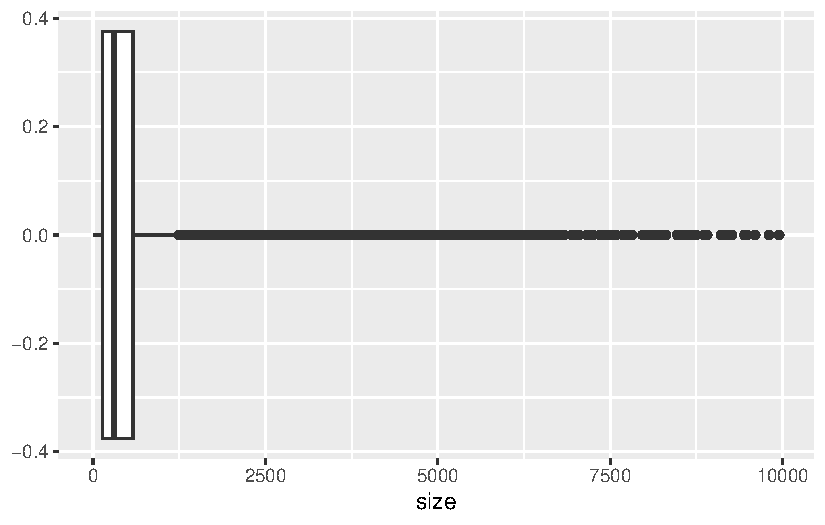
\includegraphics{scripts/02_dataViz/class3_files/figure-pdf/unnamed-chunk-14-3.pdf}

\begin{Shaded}
\begin{Highlighting}[]
\DocumentationTok{\#\# violin plot}
\FunctionTok{ggplot}\NormalTok{(variants, }\FunctionTok{aes}\NormalTok{(}\AttributeTok{x =}\NormalTok{ size)) }\SpecialCharTok{+}
  \FunctionTok{geom\_violin}\NormalTok{(}\FunctionTok{aes}\NormalTok{(}\AttributeTok{y =} \DecValTok{1}\NormalTok{)) }
\end{Highlighting}
\end{Shaded}

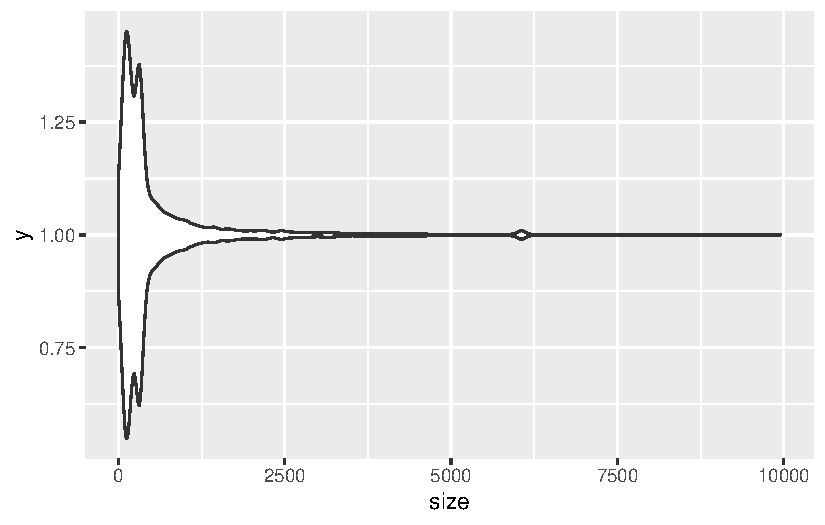
\includegraphics{scripts/02_dataViz/class3_files/figure-pdf/unnamed-chunk-14-4.pdf}

\begin{Shaded}
\begin{Highlighting}[]
\CommentTok{\# violin plots are meant to compare categories, but we can tell it we only want one plot by setting the aesthetic of \textasciigrave{}y\textasciigrave{} to the value 1}
\end{Highlighting}
\end{Shaded}

Try adding labels and titles described before. You can also easily
change the look of ggplots with different themes, try adding
\texttt{theme\_} and look at the different autofill options. See more
about built-in themes
\href{https://ggplot2.tidyverse.org/reference/ggtheme.html}{here} and
more ways to customize themes
\href{https://ggplot2.tidyverse.org/reference/ggtheme.html}{here}.

\begin{Shaded}
\begin{Highlighting}[]
\FunctionTok{ggplot}\NormalTok{(variants, }\FunctionTok{aes}\NormalTok{(}\AttributeTok{x =}\NormalTok{ size)) }\SpecialCharTok{+}
  \FunctionTok{geom\_density}\NormalTok{() }\SpecialCharTok{+}
  \FunctionTok{theme\_classic}\NormalTok{()}
\end{Highlighting}
\end{Shaded}

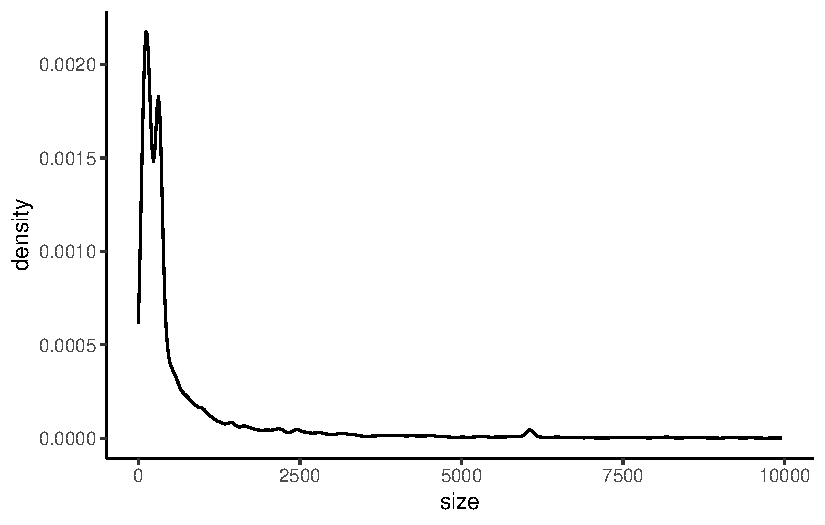
\includegraphics{scripts/02_dataViz/class3_files/figure-pdf/unnamed-chunk-15-1.pdf}

\subsection{Continuous vs Categorical}\label{continuous-vs-categorical}

Sometimes we want to see how the counts or the distribution of a
continuous variable change between different categorical groups. Often,
we use a barplot for this, but there are several other plot types we can
use

\begin{longtable}[]{@{}
  >{\raggedright\arraybackslash}p{(\columnwidth - 4\tabcolsep) * \real{0.3333}}
  >{\raggedright\arraybackslash}p{(\columnwidth - 4\tabcolsep) * \real{0.3333}}
  >{\raggedright\arraybackslash}p{(\columnwidth - 4\tabcolsep) * \real{0.3333}}@{}}
\toprule\noalign{}
\begin{minipage}[b]{\linewidth}\raggedright
Plot Type
\end{minipage} & \begin{minipage}[b]{\linewidth}\raggedright
Base R Function
\end{minipage} & \begin{minipage}[b]{\linewidth}\raggedright
ggplot Function
\end{minipage} \\
\midrule\noalign{}
\endhead
\bottomrule\noalign{}
\endlastfoot
bar plot & \texttt{barplot(name\ =\ cat\_var,\ value\ =\ cont\_var)} &
\texttt{geom\_bar()} \\
boxplots & \texttt{boxplot(cont\_var\ \textasciitilde{}\ cat\_var)} &
\texttt{geom\_boxplot()} \\
violin plots & not available & \texttt{geom\_violin()} \\
\end{longtable}

where \texttt{cont\_var} is the continuous variable and
\texttt{cat\_var} is the categorical variable.

\subsubsection{Base R}\label{base-r-2}

In base R, if we want to plot a numeric by a categorical variable, we
will use the \texttt{\textasciitilde{}} symbol to represent ``by''

For example, if we wanted to plot size by strand, we would do

\begin{Shaded}
\begin{Highlighting}[]
\FunctionTok{boxplot}\NormalTok{(variants}\SpecialCharTok{$}\NormalTok{size }\SpecialCharTok{\textasciitilde{}}\NormalTok{ variants}\SpecialCharTok{$}\NormalTok{type)}
\end{Highlighting}
\end{Shaded}

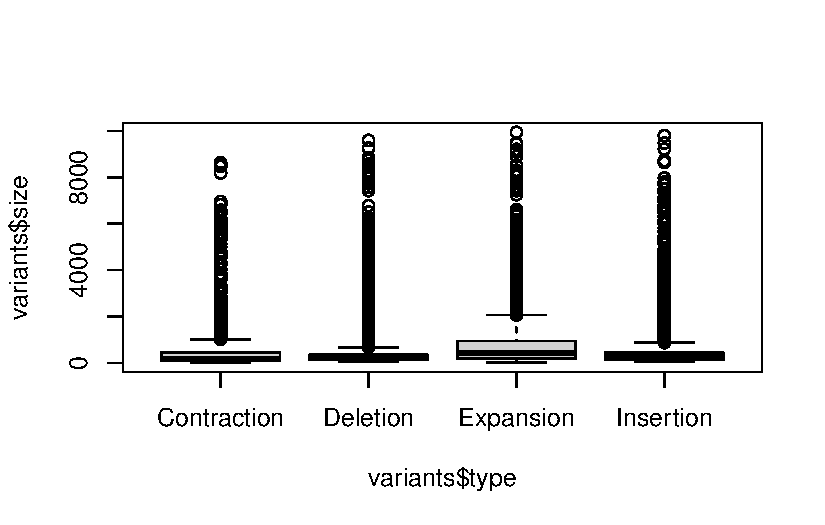
\includegraphics{scripts/02_dataViz/class3_files/figure-pdf/unnamed-chunk-16-1.pdf}

To make a barplot, we have to first count how many instances there are
of each category using the \texttt{table()} function. First, we start
with subsetting our data to only the columns we are interested in, then
we pass this smaller dataset into the \texttt{table()} function.

\begin{Shaded}
\begin{Highlighting}[]
\CommentTok{\# subset all rows, only column "type"}
\NormalTok{smallData }\OtherTok{\textless{}{-}}\NormalTok{ variants[,}\StringTok{"type"}\NormalTok{]}
\NormalTok{variantsCount }\OtherTok{\textless{}{-}} \FunctionTok{table}\NormalTok{(smallData)}
\end{Highlighting}
\end{Shaded}

Then, we use the \texttt{barplot()} function, setting the
\texttt{height} of bars to the counts in the new table, and the
\texttt{name} of the bars to the names of the table. The height of the
bars is the total summed size for each variant type.

\begin{Shaded}
\begin{Highlighting}[]
\FunctionTok{barplot}\NormalTok{(}\AttributeTok{height =}\NormalTok{ variantsCount, }\AttributeTok{names =} \FunctionTok{names}\NormalTok{(variantsCount))}
\end{Highlighting}
\end{Shaded}

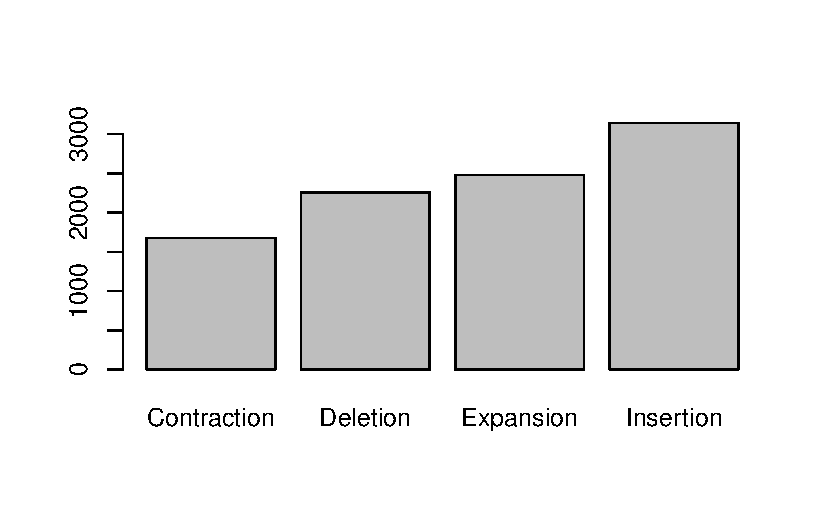
\includegraphics{scripts/02_dataViz/class3_files/figure-pdf/unnamed-chunk-18-1.pdf}

\subsubsection{ggplot}\label{ggplot-2}

When using ggplot, the total counts per category will be calculated for
us. So, we can create a base plot, setting x to the categorical variable
and y to the continuous variable, then add \texttt{+geom\_boxplot()} to
make a boxplot.

\begin{Shaded}
\begin{Highlighting}[]
\DocumentationTok{\#\# density}
\FunctionTok{ggplot}\NormalTok{(variants, }\FunctionTok{aes}\NormalTok{(}\AttributeTok{x =}\NormalTok{ type, }\AttributeTok{y =}\NormalTok{ size)) }\SpecialCharTok{+}
  \FunctionTok{geom\_boxplot}\NormalTok{()}
\end{Highlighting}
\end{Shaded}

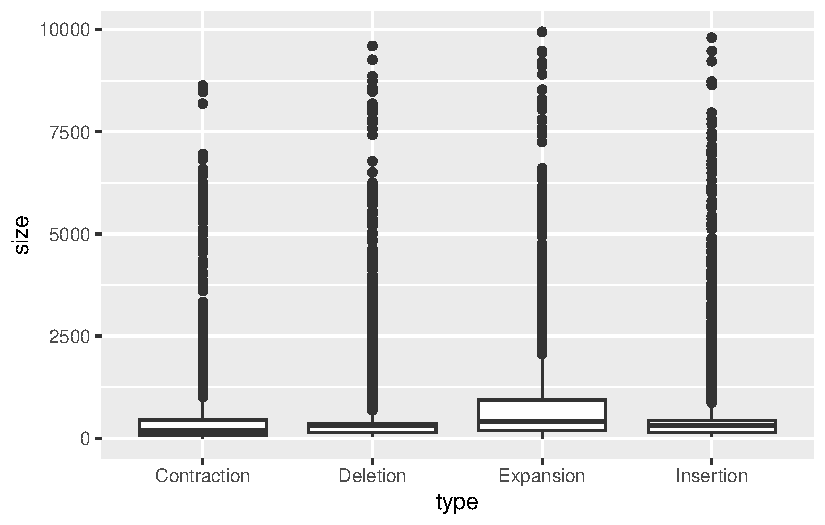
\includegraphics{scripts/02_dataViz/class3_files/figure-pdf/unnamed-chunk-19-1.pdf}

To make a barplot, we need to give it a bit more information. The height
of the barplot is based on certain statistics, such as sum or mean.
Since these are summary statistics, we will add
\texttt{stat\ =\ "summary"} and \texttt{fun\ =\ "mean"} if we want the
bar height to relate to the means of each category. How does this
compare to the sums?

\begin{Shaded}
\begin{Highlighting}[]
\DocumentationTok{\#\# boxplot}
\FunctionTok{ggplot}\NormalTok{(variants, }\FunctionTok{aes}\NormalTok{(}\AttributeTok{x =}\NormalTok{ type, }\AttributeTok{y =}\NormalTok{ size)) }\SpecialCharTok{+}
  \FunctionTok{geom\_bar}\NormalTok{(}\AttributeTok{stat =} \StringTok{"summary"}\NormalTok{, }\AttributeTok{fun =} \StringTok{"mean"}\NormalTok{)}
\end{Highlighting}
\end{Shaded}

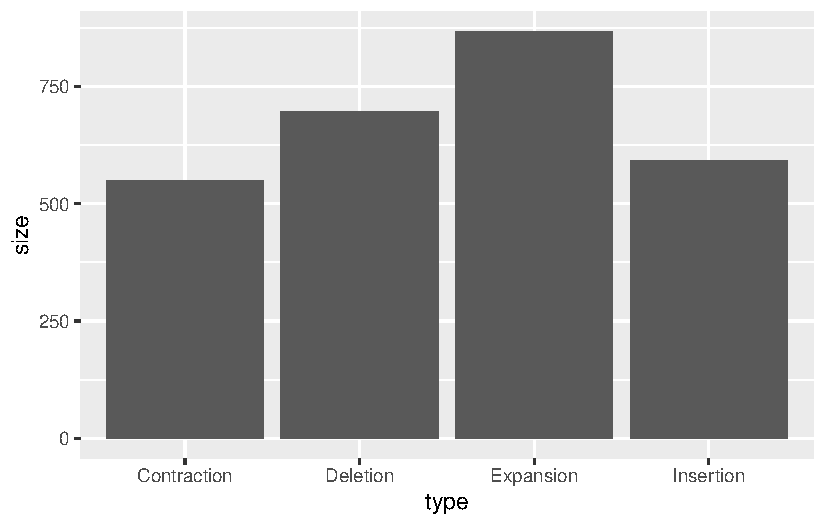
\includegraphics{scripts/02_dataViz/class3_files/figure-pdf/unnamed-chunk-20-1.pdf}

\section{Additional Resources}\label{additional-resources}

Try changing the colors using one of these tutorials:

\url{http://www.sthda.com/english/wiki/wiki.php?title=ggplot2-colors-how-to-change-colors-automatically-and-manually}

\href{https://www.datanovia.com/en/blog/ggplot-colors-best-tricks-you-will-love/\#:~:text=Change\%20ggplot\%20colors\%20by\%20assigning,or\%20to\%20the\%20fill\%20arguments.}{https://www.datanovia.com/en/blog/ggplot-colors-best-tricks-you-will-love}

\bookmarksetup{startatroot}

\chapter{Applying Visualization
Methods}\label{applying-visualization-methods}

Data Visualization, Day 2

\hfill\break

\section{Introduction}\label{introduction-2}

Welcome to Day 2 of our data visualization journey! Today, we'll dive
deeper into the world of visualizing data using the \textbf{Palmer
Penguins dataset}. This dataset provides insights into penguins in the
Palmer Archipelago, and it's a perfect opportunity for us to practice
and hone our visualization skills.

\begin{itemize}
\tightlist
\item
  This session is an opportunity to:

  \begin{itemize}
  \tightlist
  \item
    Independently code visualizations.
  \item
    Learn how to troubleshoot issues that arise.
  \item
    Explore data in a hands-on manner.
  \end{itemize}
\item
  We will also teach several new data visualization tricks:

  \begin{itemize}
  \tightlist
  \item
    Changing shapes of points.
  \item
    Customizing figure legends.
  \item
    Using \texttt{facet\_grid} for comparing many aspects of data
    simultaneously.
  \item
    Other advanced plotting tricks.
  \end{itemize}
\item
  Approach this session with curiosity and an adventurous spirit:

  \begin{itemize}
  \tightlist
  \item
    Experiment with different plot types.
  \item
    Play with colors and styles.
  \item
    Let creativity guide your visual storytelling.
  \end{itemize}
\item
  Questions are welcome. Let's make some pretty pictures!
\end{itemize}

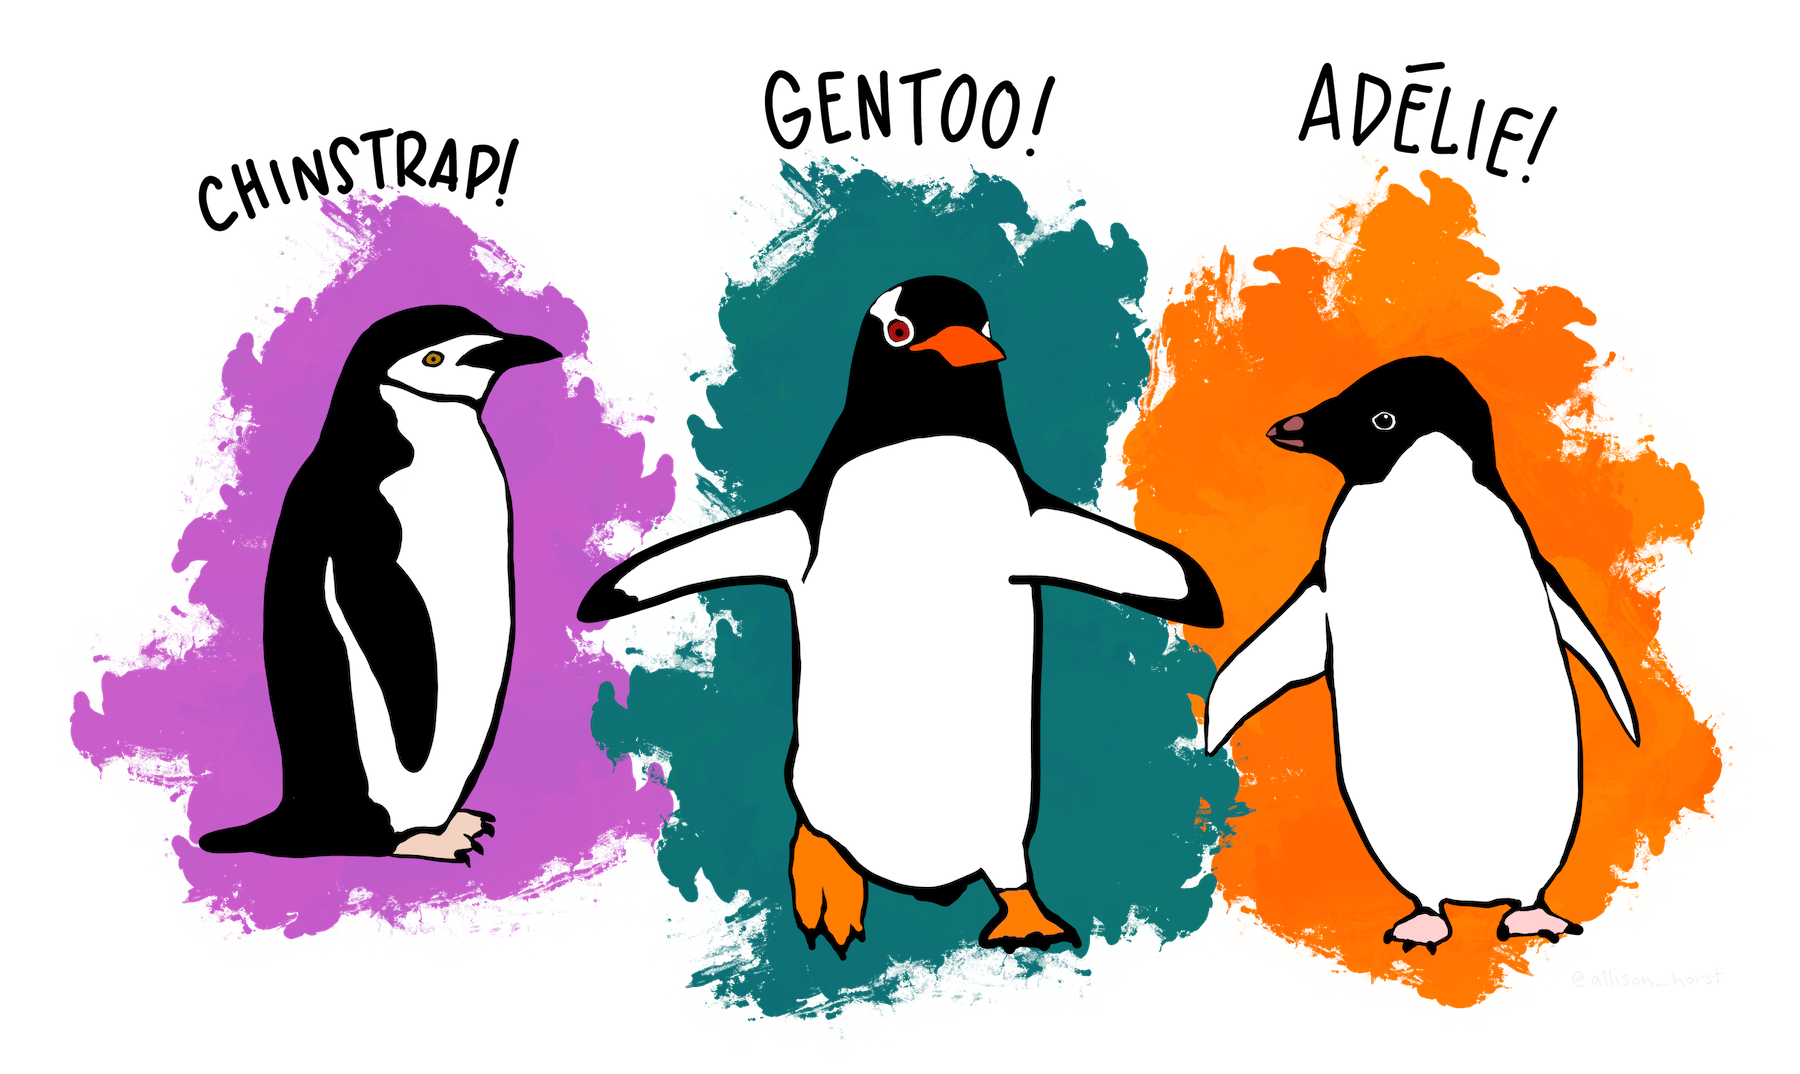
\includegraphics{scripts/02_dataViz/DataVizDay2-files/lter_penguins.png}
The Palmer Archipelago penguins. Artwork by @allison\_horst.

\section{Objectives of Data Visualization: Class
2}\label{objectives-of-data-visualization-class-2}

\begin{itemize}
\item
  Apply objectives from Class 1 to a new dataset
\item
  Create a plot from (almost) scratch, using tools (Google, Stack
  Overflow) to help you
\item
  Get a feel for the differences between creating plots in Base R and
  \texttt{ggplot}.
\end{itemize}

\section{Dataset Overview}\label{dataset-overview}

First we load necessary packages. If the \texttt{palmerpenguins} package
is not installed, we can install it by un-commenting
``install.packages'' below.

\begin{tcolorbox}[enhanced jigsaw, bottomtitle=1mm, bottomrule=.15mm, toprule=.15mm, opacityback=0, leftrule=.75mm, breakable, colback=white, toptitle=1mm, left=2mm, coltitle=black, titlerule=0mm, opacitybacktitle=0.6, title=\textcolor{quarto-callout-tip-color}{\faLightbulb}\hspace{0.5em}{Tip -- Suppress Package Startup Messages}, rightrule=.15mm, arc=.35mm, colframe=quarto-callout-tip-color-frame, colbacktitle=quarto-callout-tip-color!10!white]

The \texttt{suppressPackageStartupMessages()} function in R is used to
prevent the display of startup messages when loading packages. This can
make your R script output cleaner and more readable, especially when
loading multiple packages.

\end{tcolorbox}

\begin{Shaded}
\begin{Highlighting}[]
\FunctionTok{suppressPackageStartupMessages}\NormalTok{(}\FunctionTok{library}\NormalTok{(tidyverse))}
\CommentTok{\#install.packages(\textquotesingle{}palmerpenguins\textquotesingle{})}
\FunctionTok{library}\NormalTok{(palmerpenguins)}
\end{Highlighting}
\end{Shaded}

The dataset includes measurements of three penguin species: Adélie,
Chinstrap, and Gentoo. The \texttt{palmerpenguins} package automatically
loads the data into an object called penguins.

First we check the data class of penguins with \texttt{class()}, and
take a look at the first few rows using \texttt{head()}.

\begin{Shaded}
\begin{Highlighting}[]
\CommentTok{\#what class is our data}
\FunctionTok{class}\NormalTok{(penguins)}
\end{Highlighting}
\end{Shaded}

\begin{verbatim}
[1] "tbl_df"     "tbl"        "data.frame"
\end{verbatim}

\begin{Shaded}
\begin{Highlighting}[]
\FunctionTok{head}\NormalTok{(penguins)}
\end{Highlighting}
\end{Shaded}

\begin{verbatim}
# A tibble: 6 x 8
  species island    bill_length_mm bill_depth_mm flipper_length_mm body_mass_g
  <fct>   <fct>              <dbl>         <dbl>             <int>       <int>
1 Adelie  Torgersen           39.1          18.7               181        3750
2 Adelie  Torgersen           39.5          17.4               186        3800
3 Adelie  Torgersen           40.3          18                 195        3250
4 Adelie  Torgersen           NA            NA                  NA          NA
5 Adelie  Torgersen           36.7          19.3               193        3450
6 Adelie  Torgersen           39.3          20.6               190        3650
# i 2 more variables: sex <fct>, year <int>
\end{verbatim}

As we can see, the dataset, which is a tibble/dataframe, contains many
numerical (lengths, depths, and masses), and categorical (species,
island, and sex) variables. It also contains a variable that could be
categorical or numerical (year).

\section{Exploratory Questions}\label{exploratory-questions}

In this section, we will take some time to ask questions about the
Palmer Penguins dataset. Asking questions is a fundamental part of data
analysis, as it guides our exploration and helps us uncover interesting
patterns and insights.

Consider the different types of questions you might ask to learn more
about this dataset. What questions can we answer using different data
types, and what kind of plots might we use to answer them?

\subsection{Some example questions}\label{some-example-questions}

If you are having trouble of thinking of questions on your own, here are
some example questions related to different combinations of numerical or
categorical variables:

\begin{tcolorbox}[enhanced jigsaw, bottomtitle=1mm, bottomrule=.15mm, toprule=.15mm, opacityback=0, leftrule=.75mm, breakable, colback=white, toptitle=1mm, left=2mm, coltitle=black, titlerule=0mm, opacitybacktitle=0.6, title=\textcolor{quarto-callout-note-color}{\faInfo}\hspace{0.5em}{Questions leading to numerical by numerical plots}, rightrule=.15mm, arc=.35mm, colframe=quarto-callout-note-color-frame, colbacktitle=quarto-callout-note-color!10!white]

\begin{itemize}
\item
  How does flipper length vary with body mass among different penguin
  species? This question explores correlations and possible factors
  influencing these traits.
\item
  Is there a relationship between the bill depth and flipper length, and
  does this relationship vary by species? This encourages explores
  multiple numerical variables and consider biological implications.
  Since we are comparing species, additional visualization tools like
  coloring points by species could aid or visualization.
\end{itemize}

\end{tcolorbox}

\begin{tcolorbox}[enhanced jigsaw, bottomtitle=1mm, bottomrule=.15mm, toprule=.15mm, opacityback=0, leftrule=.75mm, breakable, colback=white, toptitle=1mm, left=2mm, coltitle=black, titlerule=0mm, opacitybacktitle=0.6, title=\textcolor{quarto-callout-note-color}{\faInfo}\hspace{0.5em}{Questions leading to categorical by numerical plot}, rightrule=.15mm, arc=.35mm, colframe=quarto-callout-note-color-frame, colbacktitle=quarto-callout-note-color!10!white]

\begin{itemize}
\item
  How does the average body mass differ across penguin species? This
  question will lead to examining differences between groups.
\item
  Does the distribution of flipper lengths differ by the island on which
  the penguins were observed? This question could be answered by a
  visauization of several separate distributions, which could overlap
  with each other.
\end{itemize}

\end{tcolorbox}

\begin{tcolorbox}[enhanced jigsaw, bottomtitle=1mm, bottomrule=.15mm, toprule=.15mm, opacityback=0, leftrule=.75mm, breakable, colback=white, toptitle=1mm, left=2mm, coltitle=black, titlerule=0mm, opacitybacktitle=0.6, title=\textcolor{quarto-callout-note-color}{\faInfo}\hspace{0.5em}{Questions related to one numerical variable}, rightrule=.15mm, arc=.35mm, colframe=quarto-callout-note-color-frame, colbacktitle=quarto-callout-note-color!10!white]

\begin{itemize}
\item
  What is the distribution of bill lengths in the Palmer Penguins
  dataset, and what might this tell us about their feeding habits?
\item
  How are body mass values distributed within each species, and what
  does this suggest about the health or environment of these
  populations?
\end{itemize}

\end{tcolorbox}

\begin{tcolorbox}[enhanced jigsaw, bottomtitle=1mm, bottomrule=.15mm, toprule=.15mm, opacityback=0, leftrule=.75mm, breakable, colback=white, toptitle=1mm, left=2mm, coltitle=black, titlerule=0mm, opacitybacktitle=0.6, title=\textcolor{quarto-callout-note-color}{\faInfo}\hspace{0.5em}{Questions related to multiple categorical variables}, rightrule=.15mm, arc=.35mm, colframe=quarto-callout-note-color-frame, colbacktitle=quarto-callout-note-color!10!white]

\begin{itemize}
\item
  How do the relationships between body mass and flipper length change
  over different years of data collection?
\item
  Can we observe any noticeable trends in bill dimensions on different
  islands, and how do these trends compare across species?
\item
  These questions require the comparision of multiple categories of
  variables, and could be usefully displayed as separate plots
  side-by-side. We will use the tool facet\_grid at the end of this
  lesson to approach such questions.
\end{itemize}

\end{tcolorbox}

\section{Making plots!}\label{making-plots}

\subsection{Warm up: numerical by numerical
plots}\label{warm-up-numerical-by-numerical-plots}

To compare two numerical variables, a scatterplot is often the simplest
and most effective plotting method. Here, we will compare the flipper
length and body mass of our penguins. Remember, the inputs to a
scatterplot are the columns of our tibble, which should be numeric,
integer, or double vectors. Lets take a look at our data with
\texttt{head()} and confirm the datatype with \texttt{class()}.

\begin{Shaded}
\begin{Highlighting}[]
\FunctionTok{head}\NormalTok{(penguins}\SpecialCharTok{$}\NormalTok{flipper\_length\_mm)}
\end{Highlighting}
\end{Shaded}

\begin{verbatim}
[1] 181 186 195  NA 193 190
\end{verbatim}

\begin{Shaded}
\begin{Highlighting}[]
\FunctionTok{class}\NormalTok{(penguins}\SpecialCharTok{$}\NormalTok{flipper\_length\_mm)}
\end{Highlighting}
\end{Shaded}

\begin{verbatim}
[1] "integer"
\end{verbatim}

\subsection{ggplot}

First we create a simple scatterplot with x and y labels in base r.

\begin{Shaded}
\begin{Highlighting}[]
\CommentTok{\#simple ggplot plot with x and y axis labeled}
\FunctionTok{ggplot}\NormalTok{(penguins, }\FunctionTok{aes}\NormalTok{(}\AttributeTok{x =}\NormalTok{ flipper\_length\_mm, }\AttributeTok{y =}\NormalTok{ body\_mass\_g,)) }\SpecialCharTok{+}
  \FunctionTok{geom\_point}\NormalTok{() }\SpecialCharTok{+}
  \FunctionTok{labs}\NormalTok{(}\AttributeTok{x =} \StringTok{"Flipper Length (cm)"}\NormalTok{, }\AttributeTok{y =} \StringTok{"Body Mass (kg)"}\NormalTok{,}
       \AttributeTok{title =} \StringTok{"Body Mass vs. Flipper Length"}\NormalTok{)}
\end{Highlighting}
\end{Shaded}

\begin{verbatim}
Warning: Removed 2 rows containing missing values or values outside the scale range
(`geom_point()`).
\end{verbatim}

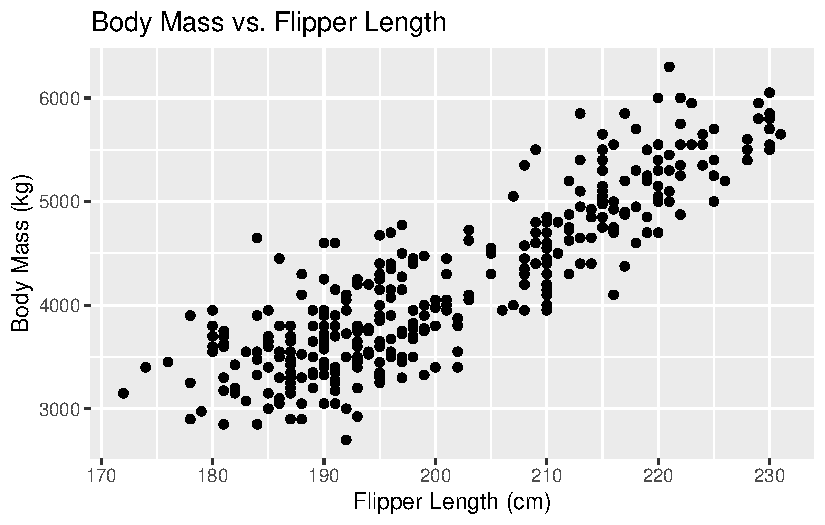
\includegraphics{scripts/02_dataViz/class4_files/figure-pdf/numvsnum2_ggplot-1.pdf}

Can we compare different species in these plots? Let's color our points
based on the species.

\begin{Shaded}
\begin{Highlighting}[]
\CommentTok{\# color dots by species}
\FunctionTok{ggplot}\NormalTok{(penguins, }\FunctionTok{aes}\NormalTok{(}\AttributeTok{x =}\NormalTok{ flipper\_length\_mm, }\AttributeTok{y =}\NormalTok{ body\_mass\_g, }\AttributeTok{color =}\NormalTok{ species)) }\SpecialCharTok{+}
  \FunctionTok{geom\_point}\NormalTok{() }\SpecialCharTok{+}
  \FunctionTok{labs}\NormalTok{(}\AttributeTok{x =} \StringTok{"Flipper Length (cm)"}\NormalTok{, }\AttributeTok{y =} \StringTok{"Body Mass (kg)"}\NormalTok{,}
       \AttributeTok{title =} \StringTok{"Body Mass vs. Flipper Length"}\NormalTok{,}
       \AttributeTok{color =} \StringTok{"Species"}\NormalTok{)}
\end{Highlighting}
\end{Shaded}

\begin{verbatim}
Warning: Removed 2 rows containing missing values or values outside the scale range
(`geom_point()`).
\end{verbatim}

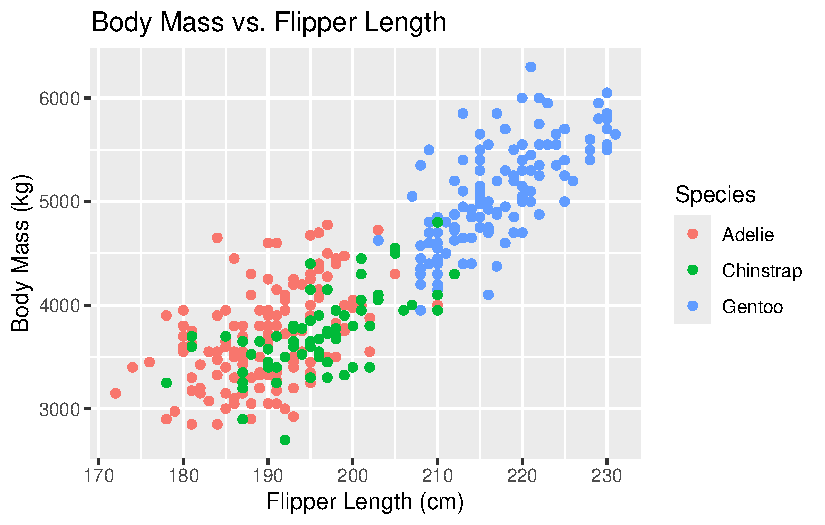
\includegraphics{scripts/02_dataViz/class4_files/figure-pdf/num_vs_num_species_ggplot-1.pdf}

\subsection{base R}

First we create a simple scatterplot with x and y labels in base r.

\begin{Shaded}
\begin{Highlighting}[]
\CommentTok{\#simple base r plot with x and y axis labeled}
\FunctionTok{plot}\NormalTok{(penguins}\SpecialCharTok{$}\NormalTok{flipper\_length\_mm, penguins}\SpecialCharTok{$}\NormalTok{body\_mass\_g,}
     \AttributeTok{xlab =} \StringTok{"Flipper Length (mm)"}\NormalTok{, }\AttributeTok{ylab =} \StringTok{"Body Mass (g)"}\NormalTok{)}
\end{Highlighting}
\end{Shaded}

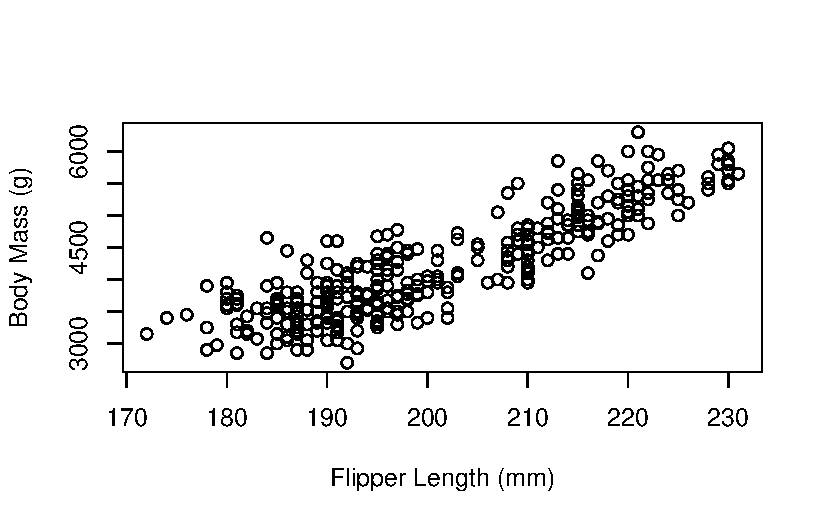
\includegraphics{scripts/02_dataViz/class4_files/figure-pdf/numvsnum2-1.pdf}

Can we compare different species in these plots? Let's color our points
based on the species.

\begin{Shaded}
\begin{Highlighting}[]
\CommentTok{\# color dots by species}
\FunctionTok{plot}\NormalTok{(penguins}\SpecialCharTok{$}\NormalTok{flipper\_length\_mm, penguins}\SpecialCharTok{$}\NormalTok{body\_mass\_g,}
     \AttributeTok{xlab =} \StringTok{"Flipper Length (mm)"}\NormalTok{, }\AttributeTok{ylab =} \StringTok{"Body Mass (g)"}\NormalTok{,}
     \AttributeTok{col =}\NormalTok{ penguins}\SpecialCharTok{$}\NormalTok{species) }
\end{Highlighting}
\end{Shaded}

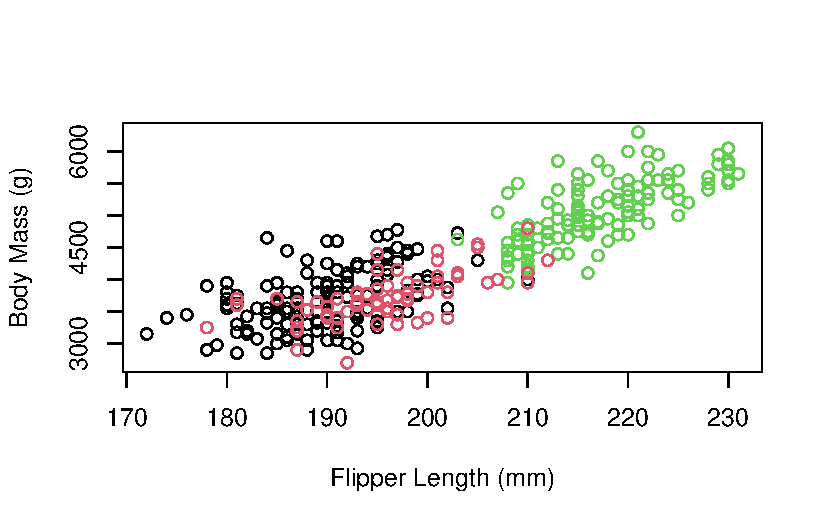
\includegraphics{scripts/02_dataViz/class4_files/figure-pdf/num_vs_num_species-1.pdf}

\begin{tcolorbox}[enhanced jigsaw, bottomtitle=1mm, bottomrule=.15mm, toprule=.15mm, opacityback=0, leftrule=.75mm, breakable, colback=white, toptitle=1mm, left=2mm, coltitle=black, titlerule=0mm, opacitybacktitle=0.6, title=\textcolor{quarto-callout-note-color}{\faInfo}\hspace{0.5em}{Why are colors specified differently in base R and ggplot?}, rightrule=.15mm, arc=.35mm, colframe=quarto-callout-note-color-frame, colbacktitle=quarto-callout-note-color!10!white]

\begin{itemize}
\item
  In base R plotting, the color for each point is specified directly
  within the \texttt{plot()} function using the col argument. This
  argument can take a vector of colors, which will be applied to the
  points in the plot. In this example, we are passing the species
  information directly to the col argument to color the points based on
  the species.
\item
  In ggplot2, the aesthetics (aes) of the plot are defined within the
  \texttt{aes()} function. The color aesthetic is specified inside the
  \texttt{aes()} function to map the species variable to the colors of
  the points. This approach follows the grammar of graphics philosophy,
  where data properties are mapped to visual properties in a structured
  way.
\item
  Both methods allow us to compare different species in the plots by
  coloring the points based on the species. However, the ggplot2
  approach is generally more flexible and powerful for creating complex
  visualizations.
\end{itemize}

\end{tcolorbox}

\subsubsection{Another way to change the colors in a ggplot--local
aesthetics}\label{another-way-to-change-the-colors-in-a-ggplotlocal-aesthetics}

In \texttt{ggplot2}, the \texttt{aes()} function is used to map data
variables to visual properties (aesthetics) of the plot. The placement
of the \texttt{color} specification can vary based on whether it is
applied globally or locally.

\begin{itemize}
\item
  Global aesthetics apply to all geoms in the plot, and are added in the
  initial \texttt{ggplot()} call (or in a stand-alone \texttt{aes()}
  layer).
\item
  Local aesthetics apply only to the geom to which they are added.
\end{itemize}

This first plot produces the same output as our original plot.

\begin{Shaded}
\begin{Highlighting}[]
\FunctionTok{ggplot}\NormalTok{(penguins, }\FunctionTok{aes}\NormalTok{(}\AttributeTok{x =}\NormalTok{ flipper\_length\_mm, }\AttributeTok{y =}\NormalTok{ body\_mass\_g)) }\SpecialCharTok{+}
  \FunctionTok{geom\_point}\NormalTok{(}\FunctionTok{aes}\NormalTok{(}\AttributeTok{color =}\NormalTok{ species)) }\SpecialCharTok{+}
  \FunctionTok{labs}\NormalTok{(}\AttributeTok{x =} \StringTok{"Flipper Length (cm)"}\NormalTok{, }\AttributeTok{y =} \StringTok{"Body Mass (kg)"}\NormalTok{,}
       \AttributeTok{title =} \StringTok{"Body Mass vs. Flipper Length"}\NormalTok{,}
       \AttributeTok{color =} \StringTok{"Species"}\NormalTok{)}
\end{Highlighting}
\end{Shaded}

\begin{verbatim}
Warning: Removed 2 rows containing missing values or values outside the scale range
(`geom_point()`).
\end{verbatim}

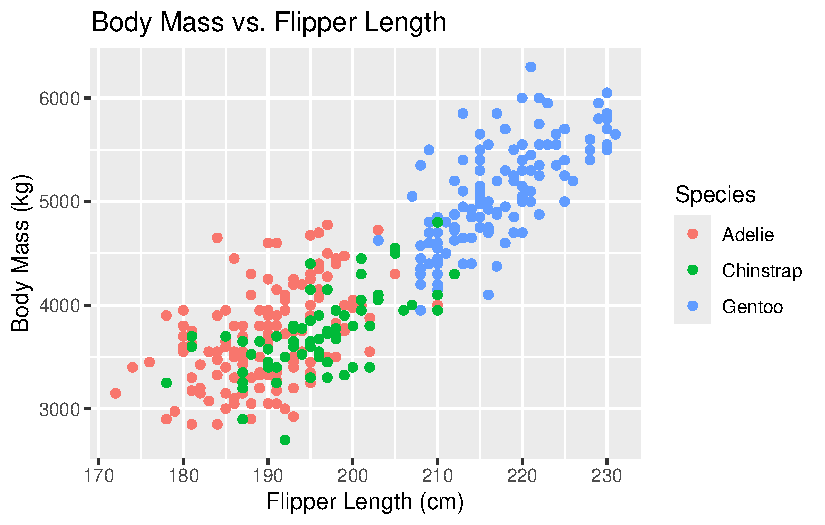
\includegraphics{scripts/02_dataViz/class4_files/figure-pdf/local_aesthetics-1.pdf}

In this second plot, the local aesthetic overrides the global one.

\begin{Shaded}
\begin{Highlighting}[]
\FunctionTok{ggplot}\NormalTok{(penguins, }\FunctionTok{aes}\NormalTok{(}\AttributeTok{x =}\NormalTok{ flipper\_length\_mm, }\AttributeTok{y =}\NormalTok{ body\_mass\_g, }\AttributeTok{color =}\NormalTok{ species)) }\SpecialCharTok{+}
  \FunctionTok{geom\_point}\NormalTok{(}\FunctionTok{aes}\NormalTok{(}\AttributeTok{color =}\NormalTok{ flipper\_length\_mm)) }\SpecialCharTok{+} \CommentTok{\# local aesthetic applied here}
  \FunctionTok{labs}\NormalTok{(}\AttributeTok{x =} \StringTok{"Flipper Length (cm)"}\NormalTok{, }\AttributeTok{y =} \StringTok{"Body Mass (kg)"}\NormalTok{,}
       \AttributeTok{title =} \StringTok{"Body Mass vs. Flipper Length"}\NormalTok{,}
       \AttributeTok{color =} \StringTok{"Species"}\NormalTok{)}
\end{Highlighting}
\end{Shaded}

\begin{verbatim}
Warning: Removed 2 rows containing missing values or values outside the scale range
(`geom_point()`).
\end{verbatim}

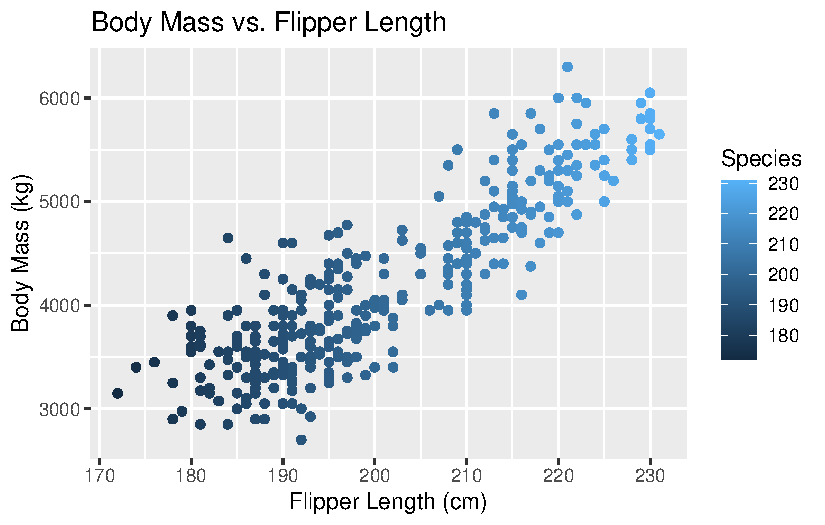
\includegraphics{scripts/02_dataViz/class4_files/figure-pdf/local_aesthetics2-1.pdf}

\subsubsection{Let's customize our
plots!}\label{lets-customize-our-plots}

Let's customize these plots some more! Here we challenge you to change
the shapes of the points for each species, add a customized legend in
the position of the plot we want, and change the size of the points.

Take 5-10 minutes to try to figure out one or more of the changes we
made to the plot:

\begin{itemize}
\tightlist
\item
  \textbf{Change the shape of the points} based on species.
\item
  \textbf{Add custom colors} for the different species.
\item
  \textbf{Change the position of the legend} to make it more visually
  pleasing.
\item
  \textbf{Add a subtitle} to the figure.
\end{itemize}

Feel free to try ggplot or base R, depending on your preference.
Practice finding this information using:

\begin{itemize}
\item
  The \href{https://rdrr.io/r/base/plot.html}{base r docs for the
  \texttt{plot()} function} or
  \href{https://ggplot2.tidyverse.org/articles/ggplot2-specs.html}{ggplot2
  docs}
\item
  Use Google to find informative articles online
  \href{https://www.statology.org/ggplot-legend-position/}{like this}
\item
  Ask a friend or instructor for help if you get stuck.
\end{itemize}

Feel free to add your own touches to the figure, and experiment with
changing the numbers and variables in the figure!

\subsection{ggplot}

\begin{verbatim}
Warning: A numeric `legend.position` argument in `theme()` was deprecated in ggplot2
3.5.0.
i Please use the `legend.position.inside` argument of `theme()` instead.
\end{verbatim}

\begin{verbatim}
Warning: Removed 2 rows containing missing values or values outside the scale range
(`geom_point()`).
\end{verbatim}

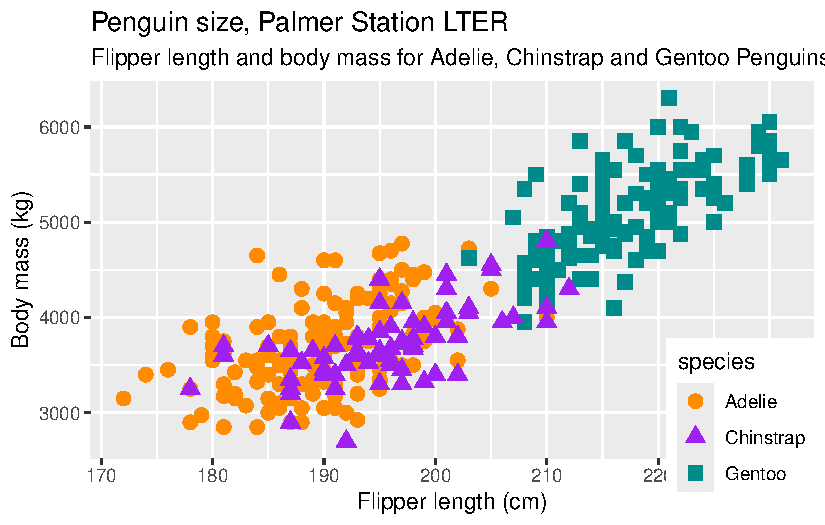
\includegraphics{scripts/02_dataViz/class4_files/figure-pdf/unnamed-chunk-2-1.pdf}

\subsection{base r}

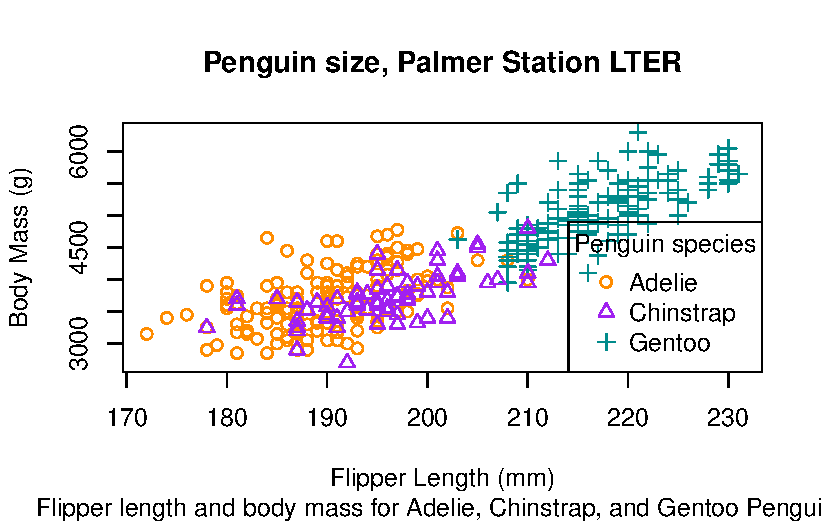
\includegraphics{scripts/02_dataViz/class4_files/figure-pdf/unnamed-chunk-3-1.pdf}

\begin{tcolorbox}[enhanced jigsaw, bottomtitle=1mm, bottomrule=.15mm, toprule=.15mm, opacityback=0, leftrule=.75mm, breakable, colback=white, toptitle=1mm, left=2mm, coltitle=black, titlerule=0mm, opacitybacktitle=0.6, title=\textcolor{quarto-callout-tip-color}{\faLightbulb}\hspace{0.5em}{Code used to make the plot--try on your own first!}, rightrule=.15mm, arc=.35mm, colframe=quarto-callout-tip-color-frame, colbacktitle=quarto-callout-tip-color!10!white]

\begin{Shaded}
\begin{Highlighting}[]
\CommentTok{\# Even more complex example with custom labels, colors, and fig legend position}
\FunctionTok{ggplot}\NormalTok{(}\AttributeTok{data =}\NormalTok{ penguins, }\FunctionTok{aes}\NormalTok{(}\AttributeTok{x =}\NormalTok{ flipper\_length\_mm, }\AttributeTok{y =}\NormalTok{ body\_mass\_g)) }\SpecialCharTok{+}
  \FunctionTok{geom\_point}\NormalTok{(}\FunctionTok{aes}\NormalTok{(}\AttributeTok{color =}\NormalTok{ species, }\AttributeTok{shape =}\NormalTok{ species), }\AttributeTok{size =} \DecValTok{3}\NormalTok{) }\SpecialCharTok{+}
  \FunctionTok{scale\_color\_manual}\NormalTok{(}\AttributeTok{values =} \FunctionTok{c}\NormalTok{(}\StringTok{"darkorange"}\NormalTok{,}\StringTok{"purple"}\NormalTok{,}\StringTok{"cyan4"}\NormalTok{)) }\SpecialCharTok{+}
  \FunctionTok{labs}\NormalTok{(}\AttributeTok{title =} \StringTok{"Penguin size, Palmer Station LTER"}\NormalTok{,}
       \AttributeTok{subtitle =} \StringTok{"Flipper length and body mass for Adelie, Chinstrap and Gentoo Penguins"}\NormalTok{,}
       \AttributeTok{x =} \StringTok{"Flipper length (cm)"}\NormalTok{,}
       \AttributeTok{y =} \StringTok{"Body mass (kg)"}\NormalTok{) }\SpecialCharTok{+}
  \FunctionTok{theme}\NormalTok{(}\AttributeTok{legend.position =} \FunctionTok{c}\NormalTok{(}\FloatTok{0.9}\NormalTok{, }\FloatTok{0.1}\NormalTok{))}

\CommentTok{\#Similar figure using base R}
\NormalTok{species\_colors }\OtherTok{\textless{}{-}} \FunctionTok{c}\NormalTok{(}\StringTok{"darkorange"}\NormalTok{, }\StringTok{"purple"}\NormalTok{, }\StringTok{"cyan4"}\NormalTok{)}

\FunctionTok{plot}\NormalTok{(penguins}\SpecialCharTok{$}\NormalTok{flipper\_length\_mm, penguins}\SpecialCharTok{$}\NormalTok{body\_mass\_g,}
     \AttributeTok{xlab =} \StringTok{"Flipper Length (mm)"}\NormalTok{, }\AttributeTok{ylab =} \StringTok{"Body Mass (g)"}\NormalTok{,}
     \AttributeTok{main =} \StringTok{"Penguin size, Palmer Station LTER"}\NormalTok{,}
     \AttributeTok{sub =} \StringTok{"Flipper length and body mass for Adelie, Chinstrap, and Gentoo Penguins"}\NormalTok{,}
     \AttributeTok{pch =} \FunctionTok{as.numeric}\NormalTok{(penguins}\SpecialCharTok{$}\NormalTok{species), }\CommentTok{\# Assign shapes based on species}
     \AttributeTok{col =}\NormalTok{ species\_colors[penguins}\SpecialCharTok{$}\NormalTok{species]) }\CommentTok{\# Assign colors based on species}

\CommentTok{\# Add legend}
\FunctionTok{legend}\NormalTok{(}\StringTok{"bottomright"}\NormalTok{, }\AttributeTok{legend =} \FunctionTok{levels}\NormalTok{(penguins}\SpecialCharTok{$}\NormalTok{species),}
       \AttributeTok{col =}\NormalTok{ species\_colors, }
       \AttributeTok{pch =} \DecValTok{1}\SpecialCharTok{:}\DecValTok{3}\NormalTok{, }\CommentTok{\#shape codes to legend}
       \AttributeTok{title =} \StringTok{"Penguin species"}\NormalTok{)}
\end{Highlighting}
\end{Shaded}

\end{tcolorbox}

\section{Time to practice!}\label{time-to-practice}

In this section, you'll have the chance to make more plots on your own.
We'll display different plots with several new features to try, and you
can use your plotting and researching skills to recreate them. This is a
great opportunity to experiment and be creative. Remember, questions are
always welcome.

\subsection{Numerical by categorical
plots}\label{numerical-by-categorical-plots}

Try making some numerical by categorical plots on your own using this
dataset! This example looks at body mass in each species, using
``jittered'' points. See if you can recreate this on your own!

\begin{tcolorbox}[enhanced jigsaw, bottomtitle=1mm, bottomrule=.15mm, toprule=.15mm, opacityback=0, leftrule=.75mm, breakable, colback=white, toptitle=1mm, left=2mm, coltitle=black, titlerule=0mm, opacitybacktitle=0.6, title=\textcolor{quarto-callout-tip-color}{\faLightbulb}\hspace{0.5em}{Hint -- a reminder of the basic syntax for boxplots}, rightrule=.15mm, arc=.35mm, colframe=quarto-callout-tip-color-frame, colbacktitle=quarto-callout-tip-color!10!white]

\section{ggplot}

\begin{Shaded}
\begin{Highlighting}[]
\CommentTok{\# ggplot boxplot of body mass values in each species}
\FunctionTok{ggplot}\NormalTok{(}\AttributeTok{data =}\NormalTok{ penguins, }\FunctionTok{aes}\NormalTok{(}\AttributeTok{x =}\NormalTok{ species, }\AttributeTok{y =}\NormalTok{ body\_mass\_g)) }\SpecialCharTok{+}
  \FunctionTok{geom\_boxplot}\NormalTok{(}\FunctionTok{aes}\NormalTok{(}\AttributeTok{color =}\NormalTok{ species), }\AttributeTok{width =} \FloatTok{0.3}\NormalTok{) }\SpecialCharTok{+}
  \FunctionTok{labs}\NormalTok{(}\AttributeTok{x =} \StringTok{"Species"}\NormalTok{,}
       \AttributeTok{y =} \StringTok{"Body mass (g)"}\NormalTok{)}
\end{Highlighting}
\end{Shaded}

\begin{verbatim}
Warning: Removed 2 rows containing non-finite outside the scale range
(`stat_boxplot()`).
\end{verbatim}

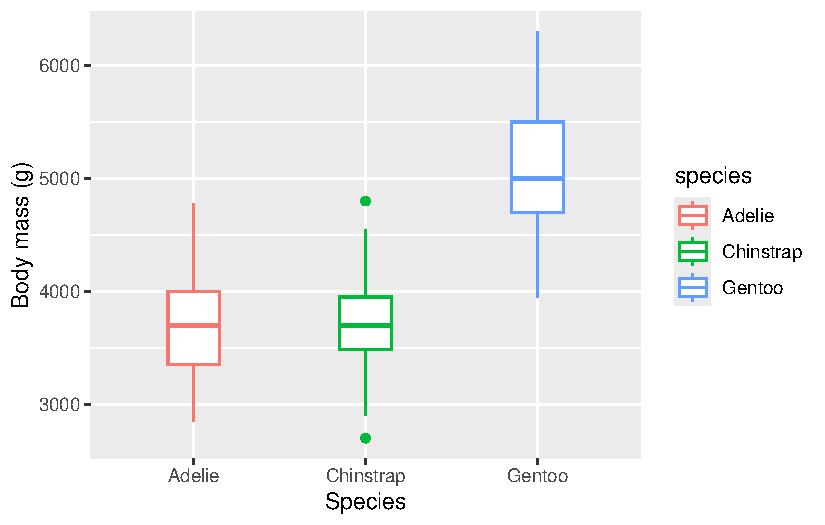
\includegraphics{scripts/02_dataViz/class4_files/figure-pdf/boxplot_ggplot-1.pdf}

\section{base r}

\begin{Shaded}
\begin{Highlighting}[]
\CommentTok{\# Base R boxplot of body mass values in each species}
\FunctionTok{boxplot}\NormalTok{(body\_mass\_g }\SpecialCharTok{\textasciitilde{}}\NormalTok{ species, }\AttributeTok{data =}\NormalTok{ penguins,}
        \AttributeTok{col =} \FunctionTok{c}\NormalTok{(}\StringTok{"darkorange"}\NormalTok{, }\StringTok{"purple"}\NormalTok{, }\StringTok{"cyan4"}\NormalTok{),}
        \AttributeTok{main =} \StringTok{"Body Mass by Penguin Species"}\NormalTok{,}
        \AttributeTok{xlab =} \StringTok{"Species"}\NormalTok{,}
        \AttributeTok{ylab =} \StringTok{"Body Mass (g)"}\NormalTok{)}
\end{Highlighting}
\end{Shaded}

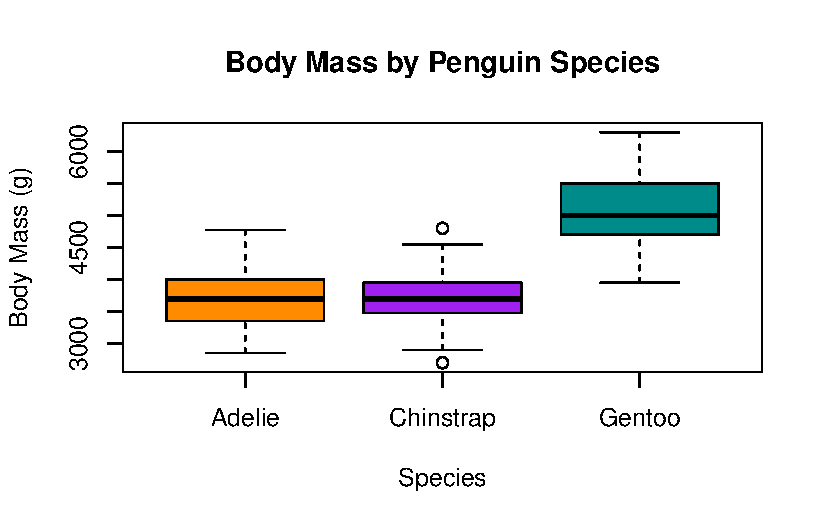
\includegraphics{scripts/02_dataViz/class4_files/figure-pdf/boxplot-1.pdf}

\end{tcolorbox}

\section{ggplot}

\begin{verbatim}
Warning: Removed 2 rows containing non-finite outside the scale range
(`stat_boxplot()`).
\end{verbatim}

\begin{verbatim}
Warning: Removed 2 rows containing missing values or values outside the scale range
(`geom_point()`).
\end{verbatim}

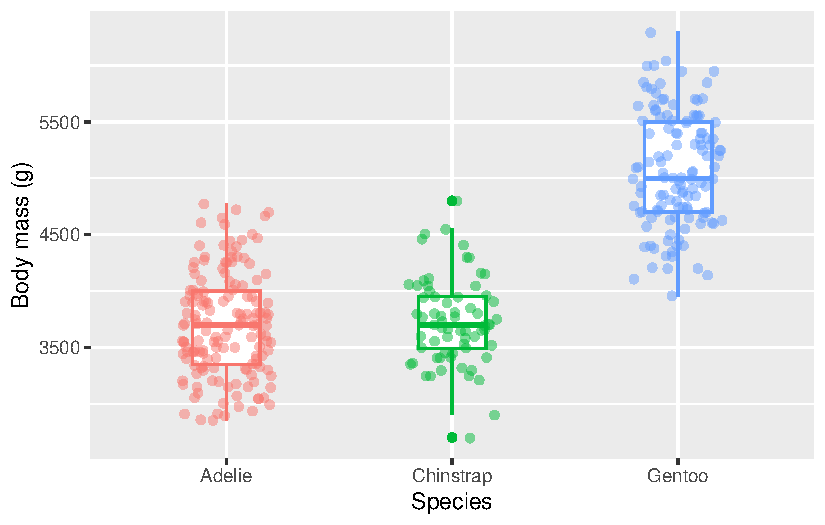
\includegraphics{scripts/02_dataViz/class4_files/figure-pdf/unnamed-chunk-5-1.pdf}

\section{base r}

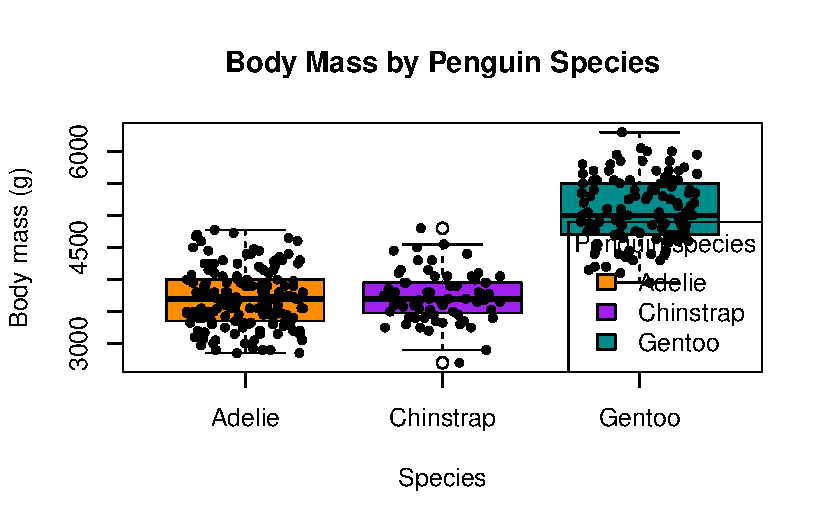
\includegraphics{scripts/02_dataViz/class4_files/figure-pdf/unnamed-chunk-6-1.pdf}

\begin{tcolorbox}[enhanced jigsaw, bottomtitle=1mm, bottomrule=.15mm, toprule=.15mm, opacityback=0, leftrule=.75mm, breakable, colback=white, toptitle=1mm, left=2mm, coltitle=black, titlerule=0mm, opacitybacktitle=0.6, title=\textcolor{quarto-callout-tip-color}{\faLightbulb}\hspace{0.5em}{How to recreate this plot--try on your own first!}, rightrule=.15mm, arc=.35mm, colframe=quarto-callout-tip-color-frame, colbacktitle=quarto-callout-tip-color!10!white]

What if we also want to see individual points in a distribution? We can
add points with ``jitter'' -- a small amount of random variation on the
x-axis -- to better visualize where the points fall.

In ggplot2, you can use the \texttt{geom\_jitter()} function to add
jittered points to your plot. This adds a small amount of random noise
to each point, making it easier to see overlapping points.

\begin{Shaded}
\begin{Highlighting}[]
\CommentTok{\# overlay the raw data points using geom\_jitter}
\FunctionTok{ggplot}\NormalTok{(}\AttributeTok{data =}\NormalTok{ penguins, }\FunctionTok{aes}\NormalTok{(}\AttributeTok{x =}\NormalTok{ species, }\AttributeTok{y =}\NormalTok{ body\_mass\_g)) }\SpecialCharTok{+}
  \FunctionTok{geom\_boxplot}\NormalTok{(}\FunctionTok{aes}\NormalTok{(}\AttributeTok{color =}\NormalTok{ species), }\AttributeTok{width =} \FloatTok{0.3}\NormalTok{, }\AttributeTok{show.legend =} \ConstantTok{FALSE}\NormalTok{) }\SpecialCharTok{+}
  \FunctionTok{geom\_jitter}\NormalTok{(}\FunctionTok{aes}\NormalTok{(}\AttributeTok{color =}\NormalTok{ species), }\AttributeTok{alpha =} \FloatTok{0.5}\NormalTok{, }\AttributeTok{show.legend =} \ConstantTok{FALSE}\NormalTok{, }
     \AttributeTok{position =} \FunctionTok{position\_jitter}\NormalTok{(}\AttributeTok{width =} \FloatTok{0.2}\NormalTok{)) }\SpecialCharTok{+}
  \FunctionTok{labs}\NormalTok{(}\AttributeTok{x =} \StringTok{"Species"}\NormalTok{,}
       \AttributeTok{y =} \StringTok{"Body mass (g)"}\NormalTok{)}
\end{Highlighting}
\end{Shaded}

In base R, you can achieve a similar effect using the \texttt{jitter()}
function. This function adds a small amount of random variation to the
data points, making overlapping points more distinguishable.

\begin{Shaded}
\begin{Highlighting}[]
\CommentTok{\# Create the boxplot}
\FunctionTok{boxplot}\NormalTok{(body\_mass\_g }\SpecialCharTok{\textasciitilde{}}\NormalTok{ species, }\AttributeTok{data =}\NormalTok{ penguins,}
        \AttributeTok{col =} \FunctionTok{c}\NormalTok{(}\StringTok{"darkorange"}\NormalTok{, }\StringTok{"purple"}\NormalTok{, }\StringTok{"cyan4"}\NormalTok{),}
        \AttributeTok{main =} \StringTok{"Body Mass by Penguin Species"}\NormalTok{,}
        \AttributeTok{xlab =} \StringTok{"Species"}\NormalTok{,}
        \AttributeTok{ylab =} \StringTok{"Body mass (g)"}\NormalTok{)}

\CommentTok{\# Add overlaid points (jittered). Factor controls the width of the points\textbackslash{}}
\CommentTok{\#cex controls their size, and pch controls the symbol}
\FunctionTok{points}\NormalTok{(}\FunctionTok{jitter}\NormalTok{(}\FunctionTok{as.numeric}\NormalTok{(penguins}\SpecialCharTok{$}\NormalTok{species), }\AttributeTok{factor =} \FloatTok{1.5}\NormalTok{),}
\NormalTok{       penguins}\SpecialCharTok{$}\NormalTok{body\_mass\_g,}
       \AttributeTok{pch =} \DecValTok{16}\NormalTok{, }\AttributeTok{cex =} \FloatTok{0.8}\NormalTok{)}

\CommentTok{\# Add custom legend (optional)}
\FunctionTok{legend}\NormalTok{(}\StringTok{"bottomright"}\NormalTok{, }\AttributeTok{legend =} \FunctionTok{levels}\NormalTok{(penguins}\SpecialCharTok{$}\NormalTok{species),}
       \AttributeTok{fill =} \FunctionTok{c}\NormalTok{(}\StringTok{"darkorange"}\NormalTok{, }\StringTok{"purple"}\NormalTok{, }\StringTok{"cyan4"}\NormalTok{),}
       \AttributeTok{title =} \StringTok{"Penguin species"}\NormalTok{)}
\end{Highlighting}
\end{Shaded}

\end{tcolorbox}

\subsection{Plotting the distribution of a numerical
variable}\label{plotting-the-distribution-of-a-numerical-variable}

If we want to loot at the distribution of one numerical variable in
detail, we could use a histogram. Here is an example of histograms that
show us the distributions of each species, using new features like
partially transparent colors and custom bar widths.

\begin{verbatim}
`stat_bin()` using `bins = 30`. Pick better value with `binwidth`.
\end{verbatim}

\begin{verbatim}
Warning: Removed 2 rows containing non-finite outside the scale range
(`stat_bin()`).
\end{verbatim}

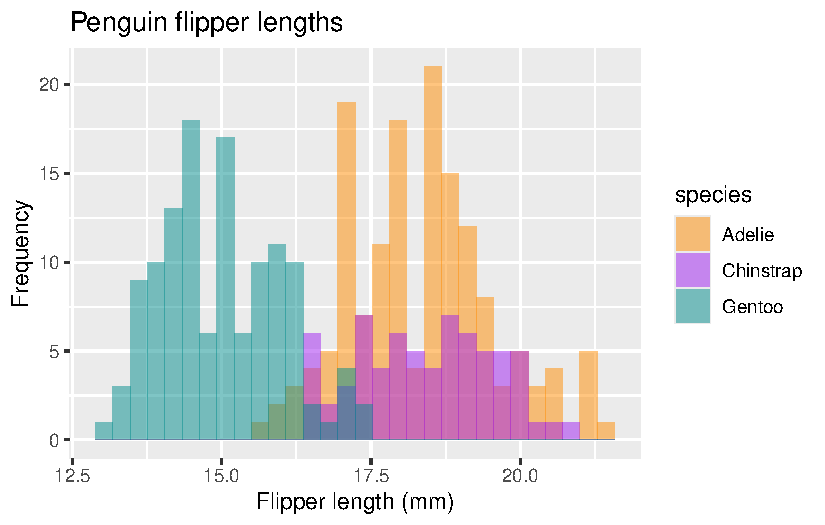
\includegraphics{scripts/02_dataViz/class4_files/figure-pdf/unnamed-chunk-9-1.pdf}

\begin{tcolorbox}[enhanced jigsaw, bottomtitle=1mm, bottomrule=.15mm, toprule=.15mm, opacityback=0, leftrule=.75mm, breakable, colback=white, toptitle=1mm, left=2mm, coltitle=black, titlerule=0mm, opacitybacktitle=0.6, title=\textcolor{quarto-callout-tip-color}{\faLightbulb}\hspace{0.5em}{Hint -- a reminder of the basic syntax for histograms}, rightrule=.15mm, arc=.35mm, colframe=quarto-callout-tip-color-frame, colbacktitle=quarto-callout-tip-color!10!white]

\section{ggplot}

\begin{Shaded}
\begin{Highlighting}[]
\CommentTok{\# a simple histogram of flipper length in ggplot}
\FunctionTok{ggplot}\NormalTok{(}\AttributeTok{data =}\NormalTok{ penguins, }\FunctionTok{aes}\NormalTok{(}\AttributeTok{x =}\NormalTok{ bill\_depth\_mm)) }\SpecialCharTok{+}
  \FunctionTok{geom\_histogram}\NormalTok{() }
\end{Highlighting}
\end{Shaded}

\begin{verbatim}
`stat_bin()` using `bins = 30`. Pick better value with `binwidth`.
\end{verbatim}

\begin{verbatim}
Warning: Removed 2 rows containing non-finite outside the scale range
(`stat_bin()`).
\end{verbatim}

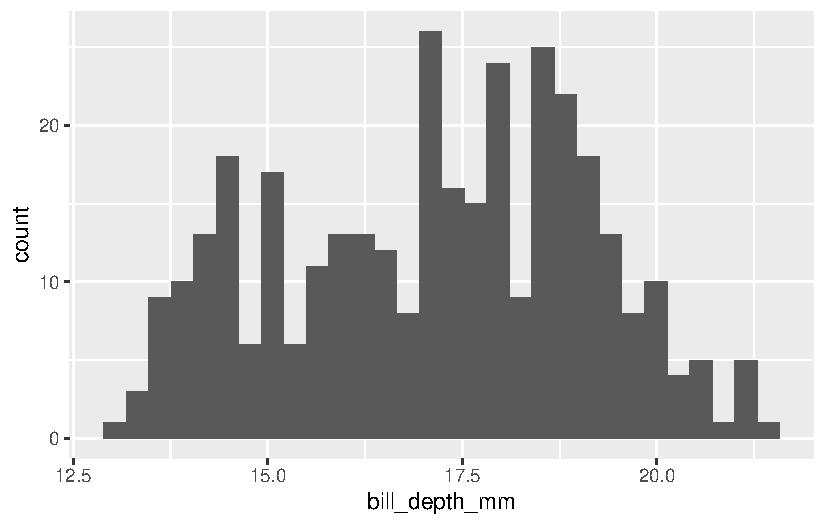
\includegraphics{scripts/02_dataViz/class4_files/figure-pdf/histogram2-1.pdf}

\section{base r}

\begin{Shaded}
\begin{Highlighting}[]
\CommentTok{\# simple histogram of flipper length}
\FunctionTok{hist}\NormalTok{(penguins}\SpecialCharTok{$}\NormalTok{bill\_depth\_mm, }\AttributeTok{main =} \StringTok{"Histogram of Penguin Bill Depth"}\NormalTok{, }\AttributeTok{xlab =} \StringTok{"Bill Depth (mm)"}\NormalTok{)}
\end{Highlighting}
\end{Shaded}

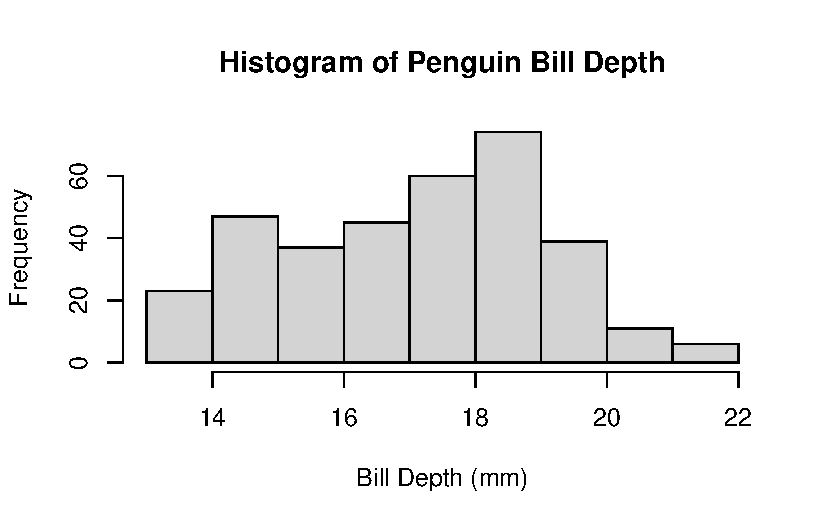
\includegraphics{scripts/02_dataViz/class4_files/figure-pdf/histogram-1.pdf}

\end{tcolorbox}

\begin{tcolorbox}[enhanced jigsaw, bottomtitle=1mm, bottomrule=.15mm, toprule=.15mm, opacityback=0, leftrule=.75mm, breakable, colback=white, toptitle=1mm, left=2mm, coltitle=black, titlerule=0mm, opacitybacktitle=0.6, title=\textcolor{quarto-callout-tip-color}{\faLightbulb}\hspace{0.5em}{How do we change bin widths for histograms?}, rightrule=.15mm, arc=.35mm, colframe=quarto-callout-tip-color-frame, colbacktitle=quarto-callout-tip-color!10!white]

\section{ggplot}

In ggplot2, you can change the number of bins in a histogram using the
bins argument within the \texttt{geom\_histogram()} function.
Alternatively, you can use the binwidth argument to specify the width of
each bin.

\begin{Shaded}
\begin{Highlighting}[]
\FunctionTok{ggplot}\NormalTok{(}\AttributeTok{data =}\NormalTok{ penguins, }\FunctionTok{aes}\NormalTok{(}\AttributeTok{x =}\NormalTok{ body\_mass\_g)) }\SpecialCharTok{+}
  \FunctionTok{geom\_histogram}\NormalTok{(}\AttributeTok{bins =} \DecValTok{30}\NormalTok{) }\SpecialCharTok{+}
  \FunctionTok{labs}\NormalTok{(}\AttributeTok{x =} \StringTok{"Body Mass (g)"}\NormalTok{, }\AttributeTok{y =} \StringTok{"Frequency"}\NormalTok{)}
\end{Highlighting}
\end{Shaded}

\begin{verbatim}
Warning: Removed 2 rows containing non-finite outside the scale range
(`stat_bin()`).
\end{verbatim}

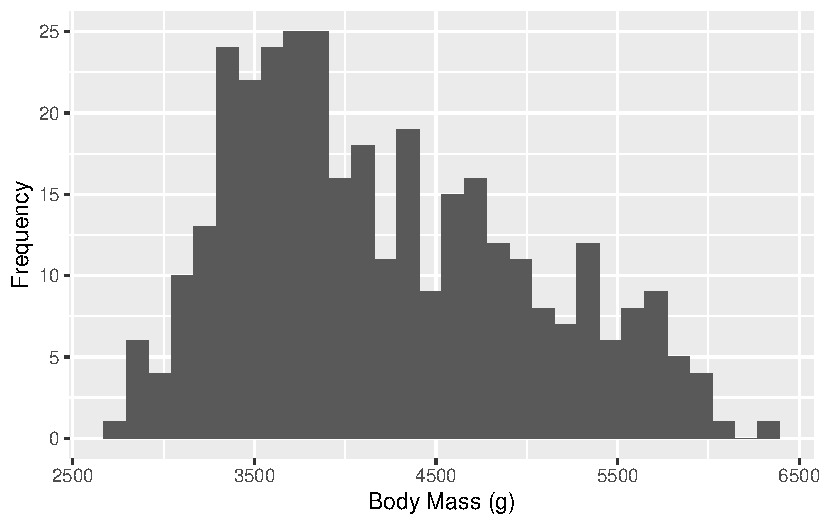
\includegraphics{scripts/02_dataViz/class4_files/figure-pdf/widths2-1.pdf}

\begin{Shaded}
\begin{Highlighting}[]
\FunctionTok{ggplot}\NormalTok{(}\AttributeTok{data =}\NormalTok{ penguins, }\FunctionTok{aes}\NormalTok{(}\AttributeTok{x =}\NormalTok{ bill\_depth\_mm)) }\SpecialCharTok{+}
  \FunctionTok{geom\_histogram}\NormalTok{(}\AttributeTok{binwidth=}\FloatTok{0.5}\NormalTok{) }
\end{Highlighting}
\end{Shaded}

\begin{verbatim}
Warning: Removed 2 rows containing non-finite outside the scale range
(`stat_bin()`).
\end{verbatim}

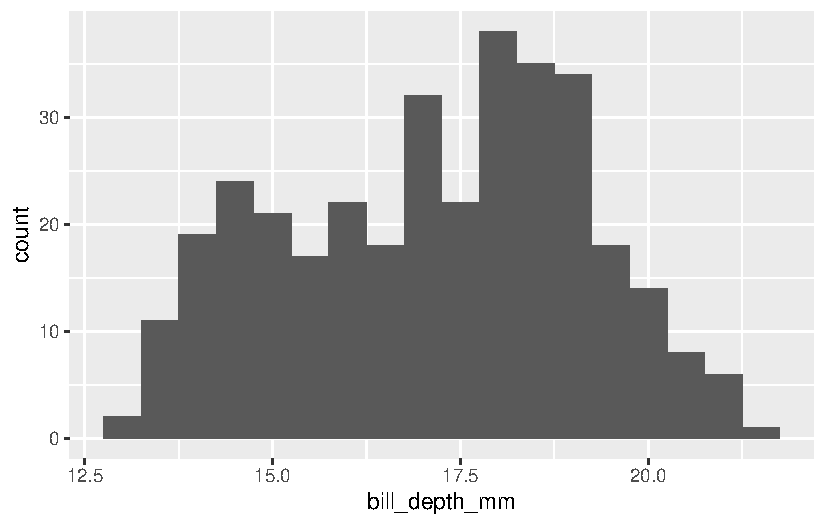
\includegraphics{scripts/02_dataViz/class4_files/figure-pdf/widths2-2.pdf}

\section{base r}

In base R, you can change the number of bins in a histogram using the
breaks argument in the \texttt{hist()} function. This argument allows
you to specify the number of bins directly, or you can pass a vector of
break points.

\begin{Shaded}
\begin{Highlighting}[]
\CommentTok{\#change the number of bins to your liking }
\FunctionTok{hist}\NormalTok{(penguins}\SpecialCharTok{$}\NormalTok{bill\_depth\_mm, }\AttributeTok{breaks =} \DecValTok{30}\NormalTok{, }\AttributeTok{main =} \StringTok{"Histogram of Penguin Bill Depth"}\NormalTok{, }\AttributeTok{xlab =} \StringTok{"Bill Depth (mm)"}\NormalTok{)}
\end{Highlighting}
\end{Shaded}

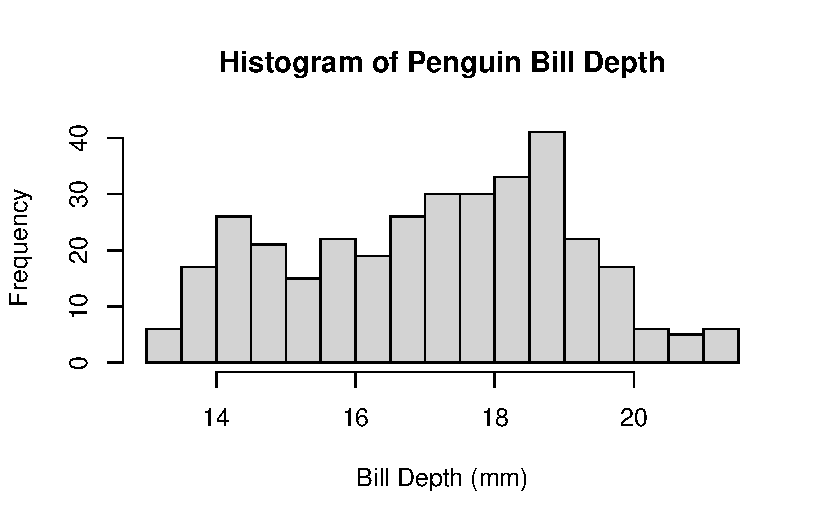
\includegraphics{scripts/02_dataViz/class4_files/figure-pdf/widths-1.pdf}

\end{tcolorbox}

\subsubsection{Challenge plot}\label{challenge-plot}

Can we \textbf{find the means} of these distributions and plot the means
on our histograms? Additionally, can we \textbf{add text} to clearly
display the mean values on the plot?

\begin{verbatim}
`stat_bin()` using `bins = 30`. Pick better value with `binwidth`.
\end{verbatim}

\begin{verbatim}
Warning: Removed 2 rows containing non-finite outside the scale range
(`stat_bin()`).
\end{verbatim}

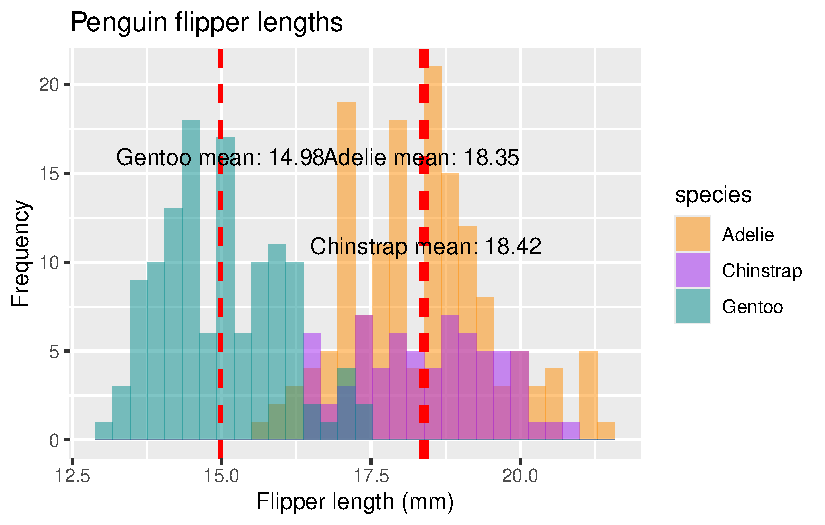
\includegraphics{scripts/02_dataViz/class4_files/figure-pdf/unnamed-chunk-10-1.pdf}

\begin{tcolorbox}[enhanced jigsaw, bottomtitle=1mm, bottomrule=.15mm, toprule=.15mm, opacityback=0, leftrule=.75mm, breakable, colback=white, toptitle=1mm, left=2mm, coltitle=black, titlerule=0mm, opacitybacktitle=0.6, title=\textcolor{quarto-callout-tip-color}{\faLightbulb}\hspace{0.5em}{Code for this image}, rightrule=.15mm, arc=.35mm, colframe=quarto-callout-tip-color-frame, colbacktitle=quarto-callout-tip-color!10!white]

\begin{Shaded}
\begin{Highlighting}[]
\CommentTok{\# Calculate the mean bill depth for each species}
\CommentTok{\# This requires some skills we will learn in Week 3!}
\NormalTok{mean\_depth }\OtherTok{\textless{}{-}}\NormalTok{ penguins }\SpecialCharTok{\%\textgreater{}\%}
  \FunctionTok{group\_by}\NormalTok{(species) }\SpecialCharTok{\%\textgreater{}\%}
  \FunctionTok{summarize}\NormalTok{(}\AttributeTok{mean\_bill\_depth =} \FunctionTok{mean}\NormalTok{(bill\_depth\_mm, }\AttributeTok{na.rm =} \ConstantTok{TRUE}\NormalTok{))}

\CommentTok{\# add a line representing the mean to the histogram}
\FunctionTok{ggplot}\NormalTok{(penguins, }\FunctionTok{aes}\NormalTok{(}\AttributeTok{x =}\NormalTok{ bill\_depth\_mm, }\AttributeTok{fill =}\NormalTok{ species)) }\SpecialCharTok{+}
  \FunctionTok{geom\_histogram}\NormalTok{(}\FunctionTok{aes}\NormalTok{(}\AttributeTok{fill =}\NormalTok{ species), }\AttributeTok{alpha =} \FloatTok{0.5}\NormalTok{, }\AttributeTok{position =} \StringTok{"identity"}\NormalTok{) }\SpecialCharTok{+}
  \FunctionTok{scale\_fill\_manual}\NormalTok{(}\AttributeTok{values =} \FunctionTok{c}\NormalTok{(}\StringTok{"darkorange"}\NormalTok{,}\StringTok{"purple"}\NormalTok{,}\StringTok{"cyan4"}\NormalTok{)) }\SpecialCharTok{+}
  \FunctionTok{labs}\NormalTok{(}\AttributeTok{x =} \StringTok{"Flipper length (mm)"}\NormalTok{,}
     \AttributeTok{y =} \StringTok{"Frequency"}\NormalTok{,}
     \AttributeTok{title =} \StringTok{"Penguin flipper lengths"}\NormalTok{)}\SpecialCharTok{+}
  \FunctionTok{geom\_vline}\NormalTok{(}\AttributeTok{data =}\NormalTok{ mean\_depth, }\FunctionTok{aes}\NormalTok{(}\AttributeTok{xintercept =}\NormalTok{ mean\_bill\_depth),}
     \AttributeTok{color =} \StringTok{"red"}\NormalTok{, }\AttributeTok{linetype =} \StringTok{"dashed"}\NormalTok{, }\AttributeTok{linewidth =} \DecValTok{1}\NormalTok{) }\SpecialCharTok{+}
  \FunctionTok{geom\_text}\NormalTok{(}\AttributeTok{data =}\NormalTok{ mean\_depth, }\FunctionTok{aes}\NormalTok{(}\AttributeTok{x =}\NormalTok{ mean\_bill\_depth, }\AttributeTok{y =} \FunctionTok{c}\NormalTok{(}\DecValTok{15}\NormalTok{,}\DecValTok{10}\NormalTok{,}\DecValTok{15}\NormalTok{),}
     \AttributeTok{label =} \FunctionTok{paste}\NormalTok{(species, }\StringTok{"mean:"}\NormalTok{, }\FunctionTok{round}\NormalTok{(mean\_bill\_depth, }\DecValTok{2}\NormalTok{))),}
     \AttributeTok{color =} \StringTok{"black"}\NormalTok{, }\AttributeTok{vjust =} \SpecialCharTok{{-}}\FloatTok{0.5}\NormalTok{, }
     \AttributeTok{hjust =} \FloatTok{0.5}\NormalTok{, }\AttributeTok{size =} \DecValTok{4}\NormalTok{) }
\end{Highlighting}
\end{Shaded}

\end{tcolorbox}

\section{Mini-Lesson: Introduction to facet\_grid in
ggplot2}\label{mini-lesson-introduction-to-facet_grid-in-ggplot2}

\subsection{Background:}\label{background}

In data visualization, particularly when dealing with complex datasets,
it's beneficial to compare subsets of data across different categories
simultaneously. ggplot2 provides various functions for creating faceted
plots, with \textbf{\texttt{facet\_grid}} being a prominent choice for
creating grids that can help in exploring interactions between
variables.

\subsection{Faceting:}\label{faceting}

Faceting refers to the strategy of splitting one plot into multiple
plots based on a factor (or factors) included in the dataset. Each plot
represents a level of the factor(s) and shares the same axis scaling and
grids, which makes them easy to compare.

The \texttt{facet\_grid} function creates a matrix of panels defined by
row and column faceting variables. The general syntax is:

\begin{Shaded}
\begin{Highlighting}[]
\FunctionTok{facet\_grid}\NormalTok{(rows }\SpecialCharTok{\textasciitilde{}}\NormalTok{ cols)}
\end{Highlighting}
\end{Shaded}

If we just want to facet by rows or just by columns, replace that spot
with a ``.''.

\begin{Shaded}
\begin{Highlighting}[]
\CommentTok{\#facet by rows}
\FunctionTok{facet\_grid}\NormalTok{(rows }\SpecialCharTok{\textasciitilde{}}\NormalTok{ .)}
\CommentTok{\#facet by cols}
\FunctionTok{facet\_grid}\NormalTok{(. }\SpecialCharTok{\textasciitilde{}}\NormalTok{ cols)}
\end{Highlighting}
\end{Shaded}

Lets take some of the plots we made earlier and facet them by the
categorical variable year! Note that in some situations it makes more
sense to facet by columns, and others by rows.

\begin{Shaded}
\begin{Highlighting}[]
\CommentTok{\# Scatter plots with facet\_grid}
\FunctionTok{ggplot}\NormalTok{(}\AttributeTok{data =}\NormalTok{ penguins, }\FunctionTok{aes}\NormalTok{(}\AttributeTok{x =}\NormalTok{ flipper\_length\_mm, }\AttributeTok{y =}\NormalTok{ body\_mass\_g)) }\SpecialCharTok{+}
  \FunctionTok{geom\_point}\NormalTok{(}\FunctionTok{aes}\NormalTok{(}\AttributeTok{color =}\NormalTok{ species, }\AttributeTok{shape =}\NormalTok{ species), }\AttributeTok{size =} \DecValTok{3}\NormalTok{) }\SpecialCharTok{+}
  \FunctionTok{scale\_color\_manual}\NormalTok{(}\AttributeTok{values =} \FunctionTok{c}\NormalTok{(}\StringTok{"darkorange"}\NormalTok{,}\StringTok{"purple"}\NormalTok{,}\StringTok{"cyan4"}\NormalTok{)) }\SpecialCharTok{+}
  \FunctionTok{labs}\NormalTok{(}\AttributeTok{title =} \StringTok{"Penguin size, Palmer Station LTER"}\NormalTok{,}
       \AttributeTok{subtitle =} \StringTok{"Flipper length and body mass for Adelie, Chinstrap and Gentoo Penguins"}\NormalTok{,}
       \AttributeTok{x =} \StringTok{"Flipper length (cm)"}\NormalTok{,}
       \AttributeTok{y =} \StringTok{"Body mass (kg)"}\NormalTok{,}
       \AttributeTok{color =} \StringTok{"Penguin species"}\NormalTok{,}
       \AttributeTok{shape =} \StringTok{"Penguin species"}\NormalTok{) }\SpecialCharTok{+}
  \FunctionTok{theme}\NormalTok{(}\AttributeTok{legend.position =} \FunctionTok{c}\NormalTok{(}\FloatTok{0.9}\NormalTok{, }\FloatTok{0.1}\NormalTok{), }\CommentTok{\# x and y on a relative scale (0{-}1)}
        \AttributeTok{plot.title.position =} \StringTok{"plot"}\NormalTok{,}
        \AttributeTok{plot.caption =} \FunctionTok{element\_text}\NormalTok{(}\AttributeTok{hjust =} \DecValTok{0}\NormalTok{, }\AttributeTok{face=} \StringTok{"italic"}\NormalTok{),}
        \AttributeTok{plot.caption.position =} \StringTok{"plot"}\NormalTok{) }\SpecialCharTok{+}
  \FunctionTok{facet\_grid}\NormalTok{(. }\SpecialCharTok{\textasciitilde{}}\NormalTok{ island) }
\end{Highlighting}
\end{Shaded}

\begin{verbatim}
Warning: Removed 2 rows containing missing values or values outside the scale range
(`geom_point()`).
\end{verbatim}

\includegraphics{scripts/02_dataViz/class4_files/figure-pdf/facet_grid-1.pdf}

\begin{Shaded}
\begin{Highlighting}[]
\CommentTok{\#Boxplots with facet\_grid}
\FunctionTok{ggplot}\NormalTok{(}\AttributeTok{data =}\NormalTok{ penguins, }\FunctionTok{aes}\NormalTok{(}\AttributeTok{x =}\NormalTok{ species, }\AttributeTok{y =}\NormalTok{ body\_mass\_g)) }\SpecialCharTok{+}
  \FunctionTok{geom\_boxplot}\NormalTok{(}\FunctionTok{aes}\NormalTok{(}\AttributeTok{color =}\NormalTok{ species), }\AttributeTok{width =} \FloatTok{0.3}\NormalTok{, }\AttributeTok{show.legend =} \ConstantTok{FALSE}\NormalTok{) }\SpecialCharTok{+}
  \FunctionTok{geom\_jitter}\NormalTok{(}\FunctionTok{aes}\NormalTok{(}\AttributeTok{color =}\NormalTok{ species), }\AttributeTok{alpha =} \FloatTok{0.5}\NormalTok{, }\AttributeTok{show.legend =} \ConstantTok{FALSE}\NormalTok{, }\AttributeTok{position =} \FunctionTok{position\_jitter}\NormalTok{(}\AttributeTok{width =} \FloatTok{0.2}\NormalTok{)) }\SpecialCharTok{+}
  \FunctionTok{labs}\NormalTok{(}\AttributeTok{x =} \StringTok{"Species"}\NormalTok{,}
       \AttributeTok{y =} \StringTok{"Body mass (g)"}\NormalTok{) }\SpecialCharTok{+}
  \FunctionTok{facet\_grid}\NormalTok{(. }\SpecialCharTok{\textasciitilde{}}\NormalTok{ year) }
\end{Highlighting}
\end{Shaded}

\begin{verbatim}
Warning: Removed 2 rows containing non-finite outside the scale range
(`stat_boxplot()`).
Removed 2 rows containing missing values or values outside the scale range
(`geom_point()`).
\end{verbatim}

\includegraphics{scripts/02_dataViz/class4_files/figure-pdf/facet_grid-2.pdf}

\begin{Shaded}
\begin{Highlighting}[]
\CommentTok{\# Histograms with facet\_grid for year}
\FunctionTok{ggplot}\NormalTok{(penguins, }\FunctionTok{aes}\NormalTok{(}\AttributeTok{x =}\NormalTok{ bill\_depth\_mm, }\AttributeTok{fill =}\NormalTok{ species)) }\SpecialCharTok{+}
  \FunctionTok{geom\_histogram}\NormalTok{(}\FunctionTok{aes}\NormalTok{(}\AttributeTok{fill =}\NormalTok{ species), }
     \AttributeTok{alpha =} \FloatTok{0.5}\NormalTok{, }
     \AttributeTok{position =} \StringTok{"identity"}\NormalTok{,}
     \AttributeTok{binwidth=}\FloatTok{0.5}\NormalTok{) }\SpecialCharTok{+}
  \FunctionTok{scale\_fill\_manual}\NormalTok{(}\AttributeTok{values =} \FunctionTok{c}\NormalTok{(}\StringTok{"darkorange"}\NormalTok{,}\StringTok{"purple"}\NormalTok{,}\StringTok{"cyan4"}\NormalTok{)) }\SpecialCharTok{+}
  \FunctionTok{labs}\NormalTok{(}\AttributeTok{x =} \StringTok{"Flipper length (mm)"}\NormalTok{,}
     \AttributeTok{y =} \StringTok{"Frequency"}\NormalTok{,}
     \AttributeTok{title =} \StringTok{"Penguin flipper lengths"}\NormalTok{)}\SpecialCharTok{+}
  \FunctionTok{geom\_vline}\NormalTok{(}\AttributeTok{data =}\NormalTok{ mean\_depth, }\FunctionTok{aes}\NormalTok{(}\AttributeTok{xintercept =}\NormalTok{ mean\_bill\_depth),}
     \AttributeTok{color =} \StringTok{"red"}\NormalTok{, }\AttributeTok{linetype =} \StringTok{"dashed"}\NormalTok{, }\AttributeTok{linewidth =} \DecValTok{1}\NormalTok{) }\SpecialCharTok{+}
  \FunctionTok{geom\_text}\NormalTok{(}\AttributeTok{data =}\NormalTok{ mean\_depth, }\FunctionTok{aes}\NormalTok{(}\AttributeTok{x =}\NormalTok{ mean\_bill\_depth, }\AttributeTok{y =} \FunctionTok{c}\NormalTok{(}\DecValTok{10}\NormalTok{,}\DecValTok{7}\NormalTok{,}\DecValTok{5}\NormalTok{,}\DecValTok{10}\NormalTok{,}\DecValTok{7}\NormalTok{,}\DecValTok{5}\NormalTok{,}\DecValTok{10}\NormalTok{,}\DecValTok{7}\NormalTok{,}\DecValTok{5}\NormalTok{),}
     \AttributeTok{label =} \FunctionTok{paste}\NormalTok{(species, }\StringTok{"mean:"}\NormalTok{, }\FunctionTok{round}\NormalTok{(mean\_bill\_depth, }\DecValTok{2}\NormalTok{))),}
     \AttributeTok{color =} \StringTok{"black"}\NormalTok{, }\AttributeTok{vjust =} \SpecialCharTok{{-}}\FloatTok{0.3}\NormalTok{, }\AttributeTok{hjust =} \FloatTok{0.5}\NormalTok{, }\AttributeTok{size =} \DecValTok{4}\NormalTok{) }\SpecialCharTok{+}
  \FunctionTok{facet\_grid}\NormalTok{(year }\SpecialCharTok{\textasciitilde{}}\NormalTok{ .) }
\end{Highlighting}
\end{Shaded}

\begin{verbatim}
Warning: Removed 2 rows containing non-finite outside the scale range
(`stat_bin()`).
\end{verbatim}

\includegraphics{scripts/02_dataViz/class4_files/figure-pdf/facet_grid-3.pdf}

\section{A useful package to make your plots colorblind
friendly}\label{a-useful-package-to-make-your-plots-colorblind-friendly}

Sometimes the plots we create are pretty, but our colorblind friends
cannot see the relationships we are trying to show with them. The
\textbf{viridis} package allows you to select from several beautiful
colorblind friendly palettes and easily incorporate them into ggplots
using \texttt{scale\_color\_viridis()}.

\begin{Shaded}
\begin{Highlighting}[]
\CommentTok{\#install.packages("viridis")}
\FunctionTok{library}\NormalTok{(viridis)}
\CommentTok{\# Scatter plots with facet\_grid}
\FunctionTok{ggplot}\NormalTok{(}\AttributeTok{data =}\NormalTok{ penguins, }\FunctionTok{aes}\NormalTok{(}\AttributeTok{x =}\NormalTok{ flipper\_length\_mm, }\AttributeTok{y =}\NormalTok{ body\_mass\_g)) }\SpecialCharTok{+}
  \FunctionTok{geom\_point}\NormalTok{(}\FunctionTok{aes}\NormalTok{(}\AttributeTok{color =}\NormalTok{ flipper\_length\_mm, }\AttributeTok{shape =}\NormalTok{ species), }\AttributeTok{size =} \DecValTok{3}\NormalTok{) }\SpecialCharTok{+}
  \FunctionTok{scale\_color\_viridis}\NormalTok{() }\SpecialCharTok{+} \CommentTok{\#scale\_color\_viridis\_d is for discrete variables like species}
  \FunctionTok{labs}\NormalTok{(}\AttributeTok{title =} \StringTok{"Penguin size, Palmer Station LTER"}\NormalTok{,}
       \AttributeTok{x =} \StringTok{"Flipper length (cm)"}\NormalTok{,}
       \AttributeTok{y =} \StringTok{"Body mass (kg)"}\NormalTok{,}
       \AttributeTok{color =} \StringTok{"Flipper length"}\NormalTok{,}
       \AttributeTok{shape =} \StringTok{"Penguin species"}\NormalTok{)}
\end{Highlighting}
\end{Shaded}

\begin{verbatim}
Warning: Removed 2 rows containing missing values or values outside the scale range
(`geom_point()`).
\end{verbatim}

\includegraphics{scripts/02_dataViz/class4_files/figure-pdf/viridis-1.pdf}

\begin{Shaded}
\begin{Highlighting}[]
\FunctionTok{ggplot}\NormalTok{(}\AttributeTok{data =}\NormalTok{ penguins, }\FunctionTok{aes}\NormalTok{(}\AttributeTok{x =}\NormalTok{ flipper\_length\_mm, }\AttributeTok{y =}\NormalTok{ body\_mass\_g)) }\SpecialCharTok{+}
  \FunctionTok{geom\_point}\NormalTok{(}\FunctionTok{aes}\NormalTok{(}\AttributeTok{color =}\NormalTok{ species, }\AttributeTok{shape =}\NormalTok{ species), }\AttributeTok{size =} \DecValTok{3}\NormalTok{) }\SpecialCharTok{+}
  \FunctionTok{scale\_color\_viridis\_d}\NormalTok{(}\AttributeTok{option=}\StringTok{"plasma"}\NormalTok{) }\SpecialCharTok{+} \CommentTok{\#try a new color scheme}
  \FunctionTok{labs}\NormalTok{(}\AttributeTok{title =} \StringTok{"Penguin size, Palmer Station LTER"}\NormalTok{,}
       \AttributeTok{x =} \StringTok{"Flipper length (cm)"}\NormalTok{,}
       \AttributeTok{y =} \StringTok{"Body mass (kg)"}\NormalTok{,}
       \AttributeTok{color =} \StringTok{"Penguin species"}\NormalTok{,}
       \AttributeTok{shape =} \StringTok{"Penguin species"}\NormalTok{)}
\end{Highlighting}
\end{Shaded}

\begin{verbatim}
Warning: Removed 2 rows containing missing values or values outside the scale range
(`geom_point()`).
\end{verbatim}

\includegraphics{scripts/02_dataViz/class4_files/figure-pdf/viridis-2.pdf}

\bookmarksetup{startatroot}

\chapter{Conclusion}\label{conclusion}

As we wrap up our exploration of data visualization, remember that the
choices you make in your visualizations should be driven by the
relationships you want to highlight in your data, while avoiding
dishonest manipulation of the data. Before you start creating your
plots, take a moment to think about what you want to understand or
communicate about your data. This will guide your decisions on which
aesthetics to use, how to customize your plots, and what story you want
your data to tell.

\section{Key Takeaways:}\label{key-takeaways}

\begin{itemize}
\tightlist
\item
  \textbf{Purpose-Driven Visualizations}: Always have a clear idea of
  the relationships and insights you want to highlight with your data.
  This focus will help you make more intentional and impactful
  visualizations.
\item
  \textbf{Customization}: Don't be afraid to experiment with different
  aesthetics and customization options. Small tweaks can significantly
  enhance the clarity and appeal of your plots.
\item
  \textbf{Clarity and Simplicity}: Aim for clarity in your
  visualizations. Make sure your plots are easy to read and interpret,
  with well-labeled axes, legends, and titles.
\item
  \textbf{Consistency}: Maintain a consistent style across your
  visualizations to create a cohesive and professional look.
\item
  \textbf{Integrity}: Ensure your visualizations are honest and
  accurate. Avoid manipulative practices that could mislead viewers or
  misrepresent the data.
\end{itemize}

Data visualization is both an art and a science. As you continue to
practice and explore different techniques, you'll develop a deeper
understanding of how to effectively communicate your data insights. Keep
experimenting, learning, and refining your skills.

\section{Some useful, free resources}\label{some-useful-free-resources}

\begin{itemize}
\tightlist
\item
  Learn how to make almost any plot type in ggplot or base r:
  \url{https://r-coder.com/}
\item
  Detailed description of ggplot functions by the authors:
  \url{https://ggplot2.tidyverse.org/articles/ggplot2.html}
\item
  Take a deep dive on the theory behind ggplot2:
  \url{https://ggplot2-book.org/}
\item
  A cookbook with basic set up and explanations for various plot types
  in base r and ggplot: \url{https://r-graphics.org/}.
\item
  Friends Don't Let Friends Make Bad Graphs:
  \url{https://github.com/cxli233/FriendsDontLetFriends}
\end{itemize}

\bookmarksetup{startatroot}

\chapter{Data Wrangling Basics}\label{data-wrangling-basics}

Data Wrangling Day 1

\hfill\break

\section{What is data wrangling?}\label{what-is-data-wrangling}

\begin{itemize}
\item
  Data wrangling, manipulation, or cleaning is the process of
  transforming data into a format that is more suitable for analysis.
  This can include removing missing values, changing the format of data,
  or combining multiple datasets.
\item
  There's rarely a single way to approach any given data-wrangling
  problem! Expanding your ``toolkit'' allows you to tackle problems from
  different angles.
\end{itemize}

\section{Objectives of Data Wrangling: Class
1}\label{objectives-of-data-wrangling-class-1}

\begin{itemize}
\item
  Be comfortable subsetting vectors and dataframes using both base R and
  tidyverse functions
\item
  Understand what tidy data is and what it looks like
\item
  Understand piping basics
\end{itemize}

\begin{tcolorbox}[enhanced jigsaw, bottomtitle=1mm, bottomrule=.15mm, toprule=.15mm, opacityback=0, leftrule=.75mm, breakable, colback=white, toptitle=1mm, left=2mm, coltitle=black, titlerule=0mm, opacitybacktitle=0.6, title=\textcolor{quarto-callout-note-color}{\faInfo}\hspace{0.5em}{Measure twice, cut once}, rightrule=.15mm, arc=.35mm, colframe=quarto-callout-note-color-frame, colbacktitle=quarto-callout-note-color!10!white]

Before you begin wrangling data, you should be able to:

\begin{itemize}
\item
  Define how you want the data to look and why
\item
  Document it well so that others (and future you!) know what you did
\item
  Know what tools you have and how to use them
\end{itemize}

\end{tcolorbox}

\section{Building a toolkit}\label{building-a-toolkit}

\subsection{Working with vectors}\label{working-with-vectors}

Pulling out specific parts of a data set is important when analyzing
with R. \textbf{Indexing}, or accessing elements, subsets data based on
numeric positions in a vector. You may remember this from the first
class. Some things to be aware of when indexing:

\begin{itemize}
\item
  Indexing uses brackets. i.e.~the 5th element in a vector will be
  returned if you run \texttt{vector{[}5{]}}.
\item
  It's helpful for getting several elements at once, or reordering data.
\end{itemize}

Here are some examples:

\begin{Shaded}
\begin{Highlighting}[]
\CommentTok{\# First, we\textquotesingle{}ll make a vector to play with}
\NormalTok{names }\OtherTok{\textless{}{-}} \FunctionTok{c}\NormalTok{(}\StringTok{"rosalind"}\NormalTok{, }\StringTok{"marie"}\NormalTok{, }\StringTok{"barbara"}\NormalTok{)}
\end{Highlighting}
\end{Shaded}

\begin{Shaded}
\begin{Highlighting}[]
\CommentTok{\# if we print the output, we\textquotesingle{}d get:}
\NormalTok{names}
\end{Highlighting}
\end{Shaded}

\begin{verbatim}
[1] "rosalind" "marie"    "barbara" 
\end{verbatim}

\begin{Shaded}
\begin{Highlighting}[]
\CommentTok{\# If we want to access the first name, we can use brackets and the position of the name in the vector:}
\NormalTok{names[}\DecValTok{1}\NormalTok{]}
\end{Highlighting}
\end{Shaded}

\begin{verbatim}
[1] "rosalind"
\end{verbatim}

\begin{Shaded}
\begin{Highlighting}[]
\CommentTok{\# This works with any position, for example the third name:}
\NormalTok{names[}\DecValTok{3}\NormalTok{]}
\end{Highlighting}
\end{Shaded}

\begin{verbatim}
[1] "barbara"
\end{verbatim}

\begin{Shaded}
\begin{Highlighting}[]
\CommentTok{\# You can index more than one position at a time too:}
\NormalTok{names[}\FunctionTok{c}\NormalTok{(}\DecValTok{1}\NormalTok{,}\DecValTok{2}\NormalTok{)]}
\end{Highlighting}
\end{Shaded}

\begin{verbatim}
[1] "rosalind" "marie"   
\end{verbatim}

\begin{Shaded}
\begin{Highlighting}[]
\CommentTok{\# Changing the order of numbers you supply changes the order of names returned}
\NormalTok{names[}\FunctionTok{c}\NormalTok{(}\DecValTok{2}\NormalTok{,}\DecValTok{1}\NormalTok{)]}
\end{Highlighting}
\end{Shaded}

\begin{verbatim}
[1] "marie"    "rosalind"
\end{verbatim}

\subsection{Working with data frames}\label{working-with-data-frames}

This works for two-dimensional structures too, like data frames and
matrices. We'd just format it as: \texttt{dataframe{[}row,column{]}}.
Let's try it out:

\begin{Shaded}
\begin{Highlighting}[]
\CommentTok{\# Make a data frame}
\NormalTok{df }\OtherTok{\textless{}{-}} \FunctionTok{data.frame}\NormalTok{(}
  \AttributeTok{name =} \FunctionTok{c}\NormalTok{(}\StringTok{"Rosalind Franklin"}\NormalTok{, }\StringTok{"Marie Curie"}\NormalTok{, }\StringTok{"Barbara McClintock"}\NormalTok{, }\StringTok{"Ada Lovelace"}\NormalTok{, }\StringTok{"Dorothy Hodgkin"}\NormalTok{, }
           \StringTok{"Lise Meitner"}\NormalTok{, }\StringTok{"Grace Hopper"}\NormalTok{, }\StringTok{"Chien{-}Shiung Wu"}\NormalTok{, }\StringTok{"Gerty Cori"}\NormalTok{, }\StringTok{"Katherine Johnson"}\NormalTok{),}
  \AttributeTok{field =} \FunctionTok{c}\NormalTok{(}\StringTok{"DNA X{-}ray crystallography"}\NormalTok{, }\StringTok{"Radioactivity"}\NormalTok{, }\StringTok{"Genetics"}\NormalTok{, }\StringTok{"Computer Programming"}\NormalTok{, }\StringTok{"X{-}ray Crystallography"}\NormalTok{, }
            \StringTok{"Nuclear Physics"}\NormalTok{, }\StringTok{"Computer Programming"}\NormalTok{, }\StringTok{"Experimental Physics"}\NormalTok{, }\StringTok{"Biochemistry"}\NormalTok{, }\StringTok{"Orbital Mechanics"}\NormalTok{),}
  \AttributeTok{school =} \FunctionTok{c}\NormalTok{(}\StringTok{"Cambridge"}\NormalTok{, }\StringTok{"Sorbonne"}\NormalTok{, }\StringTok{"Cornell"}\NormalTok{, }\StringTok{"University of London"}\NormalTok{, }\StringTok{"Oxford"}\NormalTok{, }
             \StringTok{"University of Berlin"}\NormalTok{, }\StringTok{"Yale"}\NormalTok{, }\StringTok{"Princeton"}\NormalTok{, }\StringTok{"Washington University"}\NormalTok{, }\StringTok{"West Virginia University"}\NormalTok{),}
  \AttributeTok{date\_of\_birth =} \FunctionTok{c}\NormalTok{(}\StringTok{"1920{-}07{-}25"}\NormalTok{, }\StringTok{"1867{-}11{-}07"}\NormalTok{, }\StringTok{"1902{-}06{-}16"}\NormalTok{, }\StringTok{"1815{-}12{-}10"}\NormalTok{, }\StringTok{"1910{-}05{-}12"}\NormalTok{, }
                    \StringTok{"1878{-}11{-}07"}\NormalTok{, }\StringTok{"1906{-}12{-}09"}\NormalTok{, }\StringTok{"1912{-}05{-}31"}\NormalTok{, }\StringTok{"1896{-}08{-}15"}\NormalTok{, }\StringTok{"1918{-}08{-}26"}\NormalTok{),}
  \AttributeTok{working\_region =} \FunctionTok{c}\NormalTok{(}\StringTok{"Western Europe"}\NormalTok{, }\StringTok{"Western Europe"}\NormalTok{, }\StringTok{"North America"}\NormalTok{, }\StringTok{"Western Europe"}\NormalTok{, }\StringTok{"Western Europe"}\NormalTok{, }\StringTok{"Western Europe"}\NormalTok{, }\StringTok{"North America"}\NormalTok{, }\StringTok{"North America"}\NormalTok{, }\StringTok{"North America"}\NormalTok{,  }\StringTok{"North America"}\NormalTok{)}
\NormalTok{)}

\CommentTok{\# To get the first row:}
\NormalTok{df[}\DecValTok{1}\NormalTok{,]}
\end{Highlighting}
\end{Shaded}

\begin{verbatim}
               name                     field    school date_of_birth
1 Rosalind Franklin DNA X-ray crystallography Cambridge    1920-07-25
  working_region
1 Western Europe
\end{verbatim}

\begin{Shaded}
\begin{Highlighting}[]
\CommentTok{\# or the first column: }
\NormalTok{df[,}\DecValTok{1}\NormalTok{]}
\end{Highlighting}
\end{Shaded}

\begin{verbatim}
 [1] "Rosalind Franklin"  "Marie Curie"        "Barbara McClintock"
 [4] "Ada Lovelace"       "Dorothy Hodgkin"    "Lise Meitner"      
 [7] "Grace Hopper"       "Chien-Shiung Wu"    "Gerty Cori"        
[10] "Katherine Johnson" 
\end{verbatim}

\begin{Shaded}
\begin{Highlighting}[]
\CommentTok{\# for specific cells: }
\NormalTok{df[}\DecValTok{2}\NormalTok{,}\DecValTok{3}\NormalTok{]}
\end{Highlighting}
\end{Shaded}

\begin{verbatim}
[1] "Sorbonne"
\end{verbatim}

\begin{Shaded}
\begin{Highlighting}[]
\CommentTok{\# We can use the column name instead of numbers:}
\NormalTok{df[}\DecValTok{2}\NormalTok{,}\StringTok{"school"}\NormalTok{]}
\end{Highlighting}
\end{Shaded}

\begin{verbatim}
[1] "Sorbonne"
\end{verbatim}

\begin{Shaded}
\begin{Highlighting}[]
\CommentTok{\# We can do the same thing by using a dollar sign:}
\NormalTok{df}\SpecialCharTok{$}\NormalTok{name}
\end{Highlighting}
\end{Shaded}

\begin{verbatim}
 [1] "Rosalind Franklin"  "Marie Curie"        "Barbara McClintock"
 [4] "Ada Lovelace"       "Dorothy Hodgkin"    "Lise Meitner"      
 [7] "Grace Hopper"       "Chien-Shiung Wu"    "Gerty Cori"        
[10] "Katherine Johnson" 
\end{verbatim}

\begin{Shaded}
\begin{Highlighting}[]
\CommentTok{\# We can also give a list of columns}
\CommentTok{\# which return in the order provided}
\NormalTok{df[,}\FunctionTok{c}\NormalTok{(}\StringTok{"school"}\NormalTok{,}\StringTok{"name"}\NormalTok{)]}
\end{Highlighting}
\end{Shaded}

\begin{verbatim}
                     school               name
1                 Cambridge  Rosalind Franklin
2                  Sorbonne        Marie Curie
3                   Cornell Barbara McClintock
4      University of London       Ada Lovelace
5                    Oxford    Dorothy Hodgkin
6      University of Berlin       Lise Meitner
7                      Yale       Grace Hopper
8                 Princeton    Chien-Shiung Wu
9     Washington University         Gerty Cori
10 West Virginia University  Katherine Johnson
\end{verbatim}

\subsection{Standard data formats and
Tidy}\label{standard-data-formats-and-tidy}

That data, and most two-dimensional data sets (data frames, matrices,
etc.) is often organized the similarly:

\begin{itemize}
\item
  Each variable is its own column
\item
  Each observation is its own row
\item
  Each value is a single cell.
\end{itemize}

\begin{figure}[H]

{\centering \includegraphics[width=1\textwidth,height=\textheight]{scripts/03_dataWrangling/wrangling-files/tidy-style.png}

}

\caption{Source: Hadley Wickham's R for Data Science, 1st Edition}

\end{figure}%

This follows the \emph{tidy data} style, an approach to handling data in
R that aims to be clear and readable.

\begin{tcolorbox}[enhanced jigsaw, bottomtitle=1mm, bottomrule=.15mm, toprule=.15mm, opacityback=0, leftrule=.75mm, breakable, colback=white, toptitle=1mm, left=2mm, coltitle=black, titlerule=0mm, opacitybacktitle=0.6, title=\textcolor{quarto-callout-note-color}{\faInfo}\hspace{0.5em}{Tidiest Universe}, rightrule=.15mm, arc=.35mm, colframe=quarto-callout-note-color-frame, colbacktitle=quarto-callout-note-color!10!white]

The bundle of tidy-associated packages is called the \texttt{tidyverse},
and it's a 🔥 hot-topic 🔥 in the R world. In fact, \texttt{ggplot} is a
package that you have already used that is part of the
\texttt{tidyverse}! Most data wrangling problems can be solved with
\texttt{tidy} or base (default) R functions. This can lead to some
headaches for beginners, as there are multiple ways to accomplish the
same thing!

\end{tcolorbox}

\subsection{\texorpdfstring{\texttt{dplyr}
verbs}{dplyr verbs}}\label{dplyr-verbs}

One of the most popular \texttt{tidyverse} packages, \texttt{dplyr},
offers a suite of helpful and readable functions for data manipulation.
Let's get started with how it can help you see your data:

\begin{Shaded}
\begin{Highlighting}[]
\NormalTok{dplyr}\SpecialCharTok{::}\FunctionTok{glimpse}\NormalTok{(df)}
\end{Highlighting}
\end{Shaded}

\begin{verbatim}
Rows: 10
Columns: 5
$ name           <chr> "Rosalind Franklin", "Marie Curie", "Barbara McClintock~
$ field          <chr> "DNA X-ray crystallography", "Radioactivity", "Genetics~
$ school         <chr> "Cambridge", "Sorbonne", "Cornell", "University of Lond~
$ date_of_birth  <chr> "1920-07-25", "1867-11-07", "1902-06-16", "1815-12-10",~
$ working_region <chr> "Western Europe", "Western Europe", "North America", "W~
\end{verbatim}

With the \texttt{glimpse} function we see that this is a data frame with
3 observations and 3 variables. We can also see the type of each
variable and the first few values.

\begin{tcolorbox}[enhanced jigsaw, bottomtitle=1mm, bottomrule=.15mm, toprule=.15mm, opacityback=0, leftrule=.75mm, breakable, colback=white, toptitle=1mm, left=2mm, coltitle=black, titlerule=0mm, opacitybacktitle=0.6, title=\textcolor{quarto-callout-tip-color}{\faLightbulb}\hspace{0.5em}{Tip}, rightrule=.15mm, arc=.35mm, colframe=quarto-callout-tip-color-frame, colbacktitle=quarto-callout-tip-color!10!white]

\texttt{dplyr} functions have a lot in common:

\begin{itemize}
\item
  The first argument is always a data frame
\item
  The following arguments typically specify which columns to operate on,
  using the variable names (without quotes)
\item
  The output is always a new data frame
\end{itemize}

\end{tcolorbox}

\begin{figure}[H]

{\centering \includegraphics[width=1\textwidth,height=\textheight]{scripts/03_dataWrangling/wrangling-files/dplyr_syntax.png}

}

\caption{Source: Joshua Ebner's A Quick Introduction to Dplyr}

\end{figure}%

The \texttt{dplyr} package has a set of functions that are used to
manipulate data frames (you may see these referred to as ``verbs'', and
it may also be helpful to think of them as verbs performing an action on
your dataframe). These functions can either act on rows
(e.g.~\texttt{filter} out specific rows by some condition) or columns
(e.g.~\texttt{select} columns XYZ). There are also functions for working
with groups (e.g.~group rows by what values they have in a column with
\texttt{group\_by}).

\section{rows}

The most important verbs that operate on rows of a dataset are
\texttt{filter()}, which changes which rows are present without changing
their order, and \texttt{arrange()}, which changes the order of the rows
without changing which are present. Both functions only affect the rows,
and the columns are left unchanged. We'll also discuss
\texttt{distinct()} which finds rows with unique values but unlike
\texttt{arrange()} and \texttt{filter()} it can also optionally modify
the columns.

More information about functions like this can be found
\href{https://r4ds.hadley.nz/data-transform\#rows}{here}.

\section{columns}

There are four important verbs that affect the columns without changing
the rows: \texttt{mutate()} creates new columns that are derived from
the existing columns, \texttt{select()} changes which columns are
present, \texttt{rename()} changes the names of the columns, and
\texttt{relocate()} changes the positions of the columns.

More information about functions like this can be found
\href{https://r4ds.hadley.nz/data-transform\#columns}{here}.

\section{groups}

\texttt{group\_by} allows you to create groups using more than one
variable.

\texttt{summarize} works on grouped objects and allows you to calculate
a single summary statistic, reducing the data frame to have a single row
for each group.

The \texttt{slice} family of functions allows you to extract specific
rows within each group

More information about functions like this can be found
\href{https://r4ds.hadley.nz/data-transform\#groups}{here}.

\begin{tcolorbox}[enhanced jigsaw, bottomtitle=1mm, bottomrule=.15mm, toprule=.15mm, opacityback=0, leftrule=.75mm, breakable, colback=white, toptitle=1mm, left=2mm, coltitle=black, titlerule=0mm, opacitybacktitle=0.6, title=\textcolor{quarto-callout-tip-color}{\faLightbulb}\hspace{0.5em}{Tip}, rightrule=.15mm, arc=.35mm, colframe=quarto-callout-tip-color-frame, colbacktitle=quarto-callout-tip-color!10!white]

\texttt{dplyr} verbs work great as a team!

\end{tcolorbox}

Although these were basic examples, hopefully you feel a little more
confident about working with vectors, and data frames using
\texttt{dplyr} verbs to clean and manipulate data. Happy Wrangling!

\subsection{Functions on functions}\label{functions-on-functions}

\subsubsection{An introduction to pipes}\label{an-introduction-to-pipes}

Data scientists often want to make many changes to their data at one
time. Typically, this means using more than one function at once.
However, the way we've been writing our scripts so far would make for
some very confusing looking code.

For example, let's use \texttt{dplyr} functions to perform two
operations on our data set of scientists: filter for those born after
1900 and then arrange them by date of birth.

\section{Writing it as separate steps}

Here we first filter and then arrange. Note that we are creating an
intermediate variable in between the steps.

\begin{Shaded}
\begin{Highlighting}[]
\CommentTok{\# Filtering for scientists born after 1900}
\NormalTok{filtered\_data }\OtherTok{\textless{}{-}} \FunctionTok{filter}\NormalTok{(df, }\FunctionTok{as.Date}\NormalTok{(date\_of\_birth) }\SpecialCharTok{\textgreater{}} \FunctionTok{as.Date}\NormalTok{(}\StringTok{"1900{-}01{-}01"}\NormalTok{))}

\CommentTok{\# Arranging the filtered data by date of birth}
\NormalTok{arranged\_data }\OtherTok{\textless{}{-}} \FunctionTok{arrange}\NormalTok{(filtered\_data, date\_of\_birth)}
\end{Highlighting}
\end{Shaded}

\section{Combining functions in one line}

We can do the same thing without creating an intermediate variable. It's
more compact but can start to get confusing if we add more functions.

\begin{Shaded}
\begin{Highlighting}[]
\NormalTok{arranged\_data }\OtherTok{\textless{}{-}} \FunctionTok{arrange}\NormalTok{(}\FunctionTok{filter}\NormalTok{(df, }\FunctionTok{as.Date}\NormalTok{(date\_of\_birth) }\SpecialCharTok{\textgreater{}} \FunctionTok{as.Date}\NormalTok{(}\StringTok{"1900{-}01{-}01"}\NormalTok{)), date\_of\_birth)}
\end{Highlighting}
\end{Shaded}

\section{Using pipes to clean up the code}

The \textbf{pipe operator}, \texttt{\textbar{}\textgreater{}}, is a tool
that can help make the script more readable. It allows us to pass the
result of one function directly into the next. Think of it as saying,
``and then..''

Let's dissect our goal: \emph{filter for those born after 1900}
\textbf{and then} \emph{arrange them by date of birth}.

\texttt{filter} is doing the \emph{filter for\ldots{}} part

\texttt{arrange} is doing the \emph{arrange them\ldots{}} part

and the pipe, \texttt{\textbar{}\textgreater{}}, is going to do the
\textbf{and then\ldots{}} part.

\begin{Shaded}
\begin{Highlighting}[]
\CommentTok{\# Using pipes}
\NormalTok{arranged\_data }\OtherTok{\textless{}{-}}\NormalTok{ df }\SpecialCharTok{|\textgreater{}}
  \FunctionTok{filter}\NormalTok{(}\FunctionTok{as.Date}\NormalTok{(date\_of\_birth) }\SpecialCharTok{\textgreater{}} \FunctionTok{as.Date}\NormalTok{(}\StringTok{"1900{-}01{-}01"}\NormalTok{)) }\SpecialCharTok{|\textgreater{}}
  \FunctionTok{arrange}\NormalTok{(date\_of\_birth)}
\end{Highlighting}
\end{Shaded}

Once you're comfortable with this style, you should be able to read it
as: Take \texttt{data} \emph{and then} \texttt{filter} by DoB \emph{and
then} \texttt{arrange} by DoB. This helps keep our code both clean and
readable.

\begin{tcolorbox}[enhanced jigsaw, bottomtitle=1mm, bottomrule=.15mm, toprule=.15mm, opacityback=0, leftrule=.75mm, breakable, colback=white, toptitle=1mm, left=2mm, coltitle=black, titlerule=0mm, opacitybacktitle=0.6, title=\textcolor{quarto-callout-tip-color}{\faLightbulb}\hspace{0.5em}{Tip}, rightrule=.15mm, arc=.35mm, colframe=quarto-callout-tip-color-frame, colbacktitle=quarto-callout-tip-color!10!white]

There are two pipe operators: \texttt{\textbar{}\textgreater{}} and
\texttt{\%\textgreater{}\%}. They work almost the exact same way.
\texttt{\%\textgreater{}\%} is from the \texttt{magrittr} package and
was the only way to pipe before version R 4.1.0. You may see
\texttt{\%\textgreater{}\%}more frequently in code from previous lab
members.

\begin{tcolorbox}[enhanced jigsaw, bottomtitle=1mm, bottomrule=.15mm, toprule=.15mm, opacityback=0, leftrule=.75mm, breakable, colback=white, toptitle=1mm, left=2mm, coltitle=black, titlerule=0mm, opacitybacktitle=0.6, title=\textcolor{quarto-callout-note-color}{\faInfo}\hspace{0.5em}{Placeholders}, rightrule=.15mm, arc=.35mm, colframe=quarto-callout-note-color-frame, colbacktitle=quarto-callout-note-color!10!white]

The \textbf{Placeholder} operator allows more control over where the
\texttt{LHS} (left hand side) is placed into the \texttt{RHS} (right
hand side) of the pipe operator.

\subsubsection{\texorpdfstring{\texttt{\%\textgreater{}\%}}{\%\textgreater\%}}

\texttt{\%\textgreater{}\%} uses \texttt{.} as its placeholder operator.
In addition to this, you may use \texttt{.} multiple times on the
\texttt{RHS}

\begin{Shaded}
\begin{Highlighting}[]
\DecValTok{3} \SpecialCharTok{\%\textgreater{}\%} \FunctionTok{head}\NormalTok{(}\AttributeTok{x =}\NormalTok{ letters, }\AttributeTok{n =}\NormalTok{ .)}
\end{Highlighting}
\end{Shaded}

\begin{verbatim}
[1] "a" "b" "c"
\end{verbatim}

\begin{Shaded}
\begin{Highlighting}[]
\DecValTok{3} \SpecialCharTok{\%\textgreater{}\%} \FunctionTok{sum}\NormalTok{(}\DecValTok{2}\NormalTok{, ., .)}
\end{Highlighting}
\end{Shaded}

\begin{verbatim}
[1] 8
\end{verbatim}

\subsubsection{\texorpdfstring{\texttt{\textbar{}\textgreater{}}}{\textbar\textgreater{}}}

\texttt{\textbar{}\textgreater{}} uses \texttt{\_} as its placeholder
operator. However, the \texttt{\_} placeholder must only be used once
and the argument must be named

\begin{Shaded}
\begin{Highlighting}[]
\DecValTok{3} \SpecialCharTok{|\textgreater{}} \FunctionTok{head}\NormalTok{(}\AttributeTok{x =}\NormalTok{ letters, }\AttributeTok{n =}\NormalTok{ \_)}
\end{Highlighting}
\end{Shaded}

\begin{verbatim}
[1] "a" "b" "c"
\end{verbatim}

\begin{Shaded}
\begin{Highlighting}[]
\DecValTok{3} \SpecialCharTok{|\textgreater{}} \FunctionTok{sum}\NormalTok{(}\DecValTok{2}\NormalTok{, \_)}
\end{Highlighting}
\end{Shaded}

\begin{verbatim}
Error: pipe placeholder can only be used as a named argument (<text>:1:6)
\end{verbatim}

\begin{Shaded}
\begin{Highlighting}[]
\NormalTok{add3 }\OtherTok{\textless{}{-}} \ControlFlowTok{function}\NormalTok{(x, y, z) x }\SpecialCharTok{+}\NormalTok{ y }\SpecialCharTok{+}\NormalTok{ z}
\DecValTok{3} \SpecialCharTok{|\textgreater{}} \FunctionTok{add3}\NormalTok{(}\DecValTok{2}\NormalTok{, }\AttributeTok{y =}\NormalTok{ \_, }\AttributeTok{z =}\NormalTok{ \_)}
\end{Highlighting}
\end{Shaded}

\begin{verbatim}
Error: pipe placeholder may only appear once (<text>:2:6)
\end{verbatim}

\end{tcolorbox}

\begin{tcolorbox}[enhanced jigsaw, bottomtitle=1mm, bottomrule=.15mm, toprule=.15mm, opacityback=0, leftrule=.75mm, breakable, colback=white, toptitle=1mm, left=2mm, coltitle=black, titlerule=0mm, opacitybacktitle=0.6, title=\textcolor{quarto-callout-note-color}{\faInfo}\hspace{0.5em}{Right Hand Side (RHS)}, rightrule=.15mm, arc=.35mm, colframe=quarto-callout-note-color-frame, colbacktitle=quarto-callout-note-color!10!white]

\subsubsection{\texorpdfstring{\texttt{\%\textgreater{}\%}}{\%\textgreater\%}}

\texttt{\%\textgreater{}\%} can take a function name on the \texttt{RHS}

\begin{Shaded}
\begin{Highlighting}[]
\NormalTok{letters }\SpecialCharTok{\%\textgreater{}\%}\NormalTok{ head}
\end{Highlighting}
\end{Shaded}

\begin{verbatim}
[1] "a" "b" "c" "d" "e" "f"
\end{verbatim}

\subsubsection{\texorpdfstring{\texttt{\textbar{}\textgreater{}}}{\textbar\textgreater{}}}

The \texttt{RHS} for \texttt{\textbar{}\textgreater{}} must be a
function with \texttt{()}

\begin{Shaded}
\begin{Highlighting}[]
\NormalTok{letters }\SpecialCharTok{|\textgreater{}}\NormalTok{ head}
\end{Highlighting}
\end{Shaded}

\begin{verbatim}
Error: The pipe operator requires a function call as RHS (<text>:1:12)
\end{verbatim}

\begin{Shaded}
\begin{Highlighting}[]
\NormalTok{letters }\SpecialCharTok{|\textgreater{}} \FunctionTok{head}\NormalTok{()}
\end{Highlighting}
\end{Shaded}

\begin{verbatim}
[1] "a" "b" "c" "d" "e" "f"
\end{verbatim}

\end{tcolorbox}

\begin{tcolorbox}[enhanced jigsaw, bottomtitle=1mm, bottomrule=.15mm, toprule=.15mm, opacityback=0, leftrule=.75mm, breakable, colback=white, toptitle=1mm, left=2mm, coltitle=black, titlerule=0mm, opacitybacktitle=0.6, title=\textcolor{quarto-callout-note-color}{\faInfo}\hspace{0.5em}{Anonymous Functions}, rightrule=.15mm, arc=.35mm, colframe=quarto-callout-note-color-frame, colbacktitle=quarto-callout-note-color!10!white]

\subsubsection{\texorpdfstring{\texttt{\%\textgreater{}\%}}{\%\textgreater\%}}

\texttt{\%\textgreater{}\%} can take expressions in curly braces
\texttt{\{\}}

\begin{Shaded}
\begin{Highlighting}[]
\NormalTok{x }\OtherTok{\textless{}{-}} \DecValTok{10}
\DecValTok{5} \SpecialCharTok{\%\textgreater{}\%}\NormalTok{ \{x }\SpecialCharTok{+}\NormalTok{ .\}}
\end{Highlighting}
\end{Shaded}

\begin{verbatim}
[1] 15
\end{verbatim}

\subsubsection{\texorpdfstring{\texttt{\textbar{}\textgreater{}}}{\textbar\textgreater{}}}

\texttt{\textbar{}\textgreater{}} must have a function call on
\texttt{RHS}

\begin{Shaded}
\begin{Highlighting}[]
\NormalTok{x }\OtherTok{\textless{}{-}} \DecValTok{10}
\DecValTok{5} \SpecialCharTok{|\textgreater{}}\NormalTok{ \{x }\SpecialCharTok{+}\NormalTok{ \_\}}
\end{Highlighting}
\end{Shaded}

\begin{verbatim}
Error: function '{' not supported in RHS call of a pipe (<text>:2:6)
\end{verbatim}

\begin{Shaded}
\begin{Highlighting}[]
\DecValTok{5} \SpecialCharTok{|\textgreater{}}\NormalTok{ \{}\ControlFlowTok{function}\NormalTok{(y) x }\SpecialCharTok{+}\NormalTok{ y\}()}
\end{Highlighting}
\end{Shaded}

\begin{verbatim}
[1] 15
\end{verbatim}

\end{tcolorbox}

To summarize, \texttt{\%\textgreater{}\%} is slightly more lenient than
\texttt{\textbar{}\textgreater{}} when it comes to the Placeholder
operator, the Right Hand Side (RHS) and Anonymous functions.

\end{tcolorbox}

\section{Case Study Introduction}\label{case-study-introduction}

Just reading about ways to manipulate data can be hard to understand
without an application. Since this course is geared towards biomedical
sciences, we thought you might find it easier if we work through an
actual research data set.

For this example, we have some data from an experiment that measured the
proportions of different cell times within mouse cardiac tissue. These
samples are from treatment vs.~control and WT (wild type) vs.~mutant.

What are some things that we, as researchers, would want to know about
our data?

\begin{itemize}
\tightlist
\item
  Did the experiment work?
\end{itemize}

\begin{tcolorbox}[enhanced jigsaw, bottomtitle=1mm, bottomrule=.15mm, toprule=.15mm, opacityback=0, leftrule=.75mm, breakable, colback=white, toptitle=1mm, left=2mm, coltitle=black, titlerule=0mm, opacitybacktitle=0.6, title=\textcolor{quarto-callout-note-color}{\faInfo}\hspace{0.5em}{Things to consider:}, rightrule=.15mm, arc=.35mm, colframe=quarto-callout-note-color-frame, colbacktitle=quarto-callout-note-color!10!white]

Check your controls or expected features!

\end{tcolorbox}

\begin{itemize}
\tightlist
\item
  Do we see differences between our experimental groups?
\end{itemize}

To get at these questions, we need to be able to manipulate our data
into the formats needed to check those features and for plotting. To
start, lets take a look at how the results are structured before we
start planning how to do the processing.

\subsection{Getting familiar with the
data}\label{getting-familiar-with-the-data}

\begin{Shaded}
\begin{Highlighting}[]
\FunctionTok{options}\NormalTok{(}\AttributeTok{digits =} \DecValTok{3}\NormalTok{)}
\CommentTok{\# Load the data. The sample IDs were stored as the first row, so lets make those the row.names}
\NormalTok{cell\_props }\OtherTok{\textless{}{-}} \FunctionTok{read.csv}\NormalTok{(}\StringTok{"wrangling{-}files/cellProportions.csv"}\NormalTok{,}
                       \AttributeTok{row.names =} \DecValTok{1}\NormalTok{)}

\FunctionTok{head}\NormalTok{(cell\_props)}
\end{Highlighting}
\end{Shaded}

\begin{verbatim}
            Cardiomyocytes Fibroblast Endothelial.Cells Macrophage
whole_2              0.652     0.0886           0.06700     0.1761
fraction_13          0.824     0.0370           0.06387     0.0692
fraction_12          0.895     0.0213           0.04436     0.0390
fraction_19          0.000     0.9983           0.00167     0.0000
fraction_18          0.000     1.0000           0.00000     0.0000
whole_16             0.820     0.0208           0.08889     0.0501
            Pericytes.SMC
whole_2           0.01672
fraction_13       0.00558
fraction_12       0.00000
fraction_19       0.00000
fraction_18       0.00000
whole_16          0.02058
\end{verbatim}

\begin{tcolorbox}[enhanced jigsaw, bottomtitle=1mm, bottomrule=.15mm, toprule=.15mm, opacityback=0, leftrule=.75mm, breakable, colback=white, toptitle=1mm, left=2mm, coltitle=black, titlerule=0mm, opacitybacktitle=0.6, title=\textcolor{quarto-callout-note-color}{\faInfo}\hspace{0.5em}{Whole vs.~Fractions}, rightrule=.15mm, arc=.35mm, colframe=quarto-callout-note-color-frame, colbacktitle=quarto-callout-note-color!10!white]

\texttt{Fraction} samples are our controls. They are supposed to be
almost completely one single cell type. They're just here to make sure
we accurately measured cell type proportions.

\texttt{Whole} samples are our test samples. They're from the
treatment/control mice, which you'd expect to have a range of cell
types.

\end{tcolorbox}

\subsection{Analysis Goals}\label{analysis-goals}

For next class, you should brainstorm some ideas for how to approach the
analysis. Try to consider these angles:

\begin{itemize}
\tightlist
\item
  What do we want to know about this data set?
\item
  What kind of visuals would we want to make to check that?
\item
  What would the data need to look like to get those visuals?
\item
  How does the data look now?
\item
  Which functions might we use to get the data from its current state to
  what we need for plotting?
\end{itemize}

In the beginning of next class, we'll chat about what ideas you had!

(Ambitious students who want to try before then will also need the
phenotype data located at \texttt{wrangling-files/cellPhenotypes.csv})

\bookmarksetup{startatroot}

\chapter{Data Wrangling with Cell Type
Proportions}\label{data-wrangling-with-cell-type-proportions}

Data Wrangling Day 2

\hfill\break

\section{Objectives of Data Wrangling: Class
2}\label{objectives-of-data-wrangling-class-2}

\begin{itemize}
\tightlist
\item
  Be able to apply the objectives covered in Data Wrangling: Class 1 to
  a new dataset
\end{itemize}

\section{Case Study}\label{case-study}

Last class, we had introduced a dataset/experiment that we would work
through. Let's remind ourselves of some of the details:

\begin{itemize}
\tightlist
\item
  We have proportions of cell types across samples
\item
  There controls made of mostly pure cell types (\texttt{fractions}) and
  experimental samples (\texttt{whole})
\item
  There are \texttt{.csv} files for both the cell type proportion data
  and the sample phenotypes
\end{itemize}

There are a few things to think about when wrangling/exploring data:

\begin{itemize}
\tightlist
\item
  What do you want to know about this data?
\item
  What kind of visuals would you want to make?
\item
  How does the data need to be formatted to get those visuals?
\item
  What are some expected features of our data?
\end{itemize}

Take a moment to talk among yourselves about this/any ideas you had
since last class!

\subsection{Getting familiar with the
data}\label{getting-familiar-with-the-data-1}

\subsubsection{Proportions Data}\label{proportions-data}

\begin{Shaded}
\begin{Highlighting}[]
\CommentTok{\# Load the data. The sample IDs were stored as the first row, so lets make those the row.names}
\NormalTok{cell\_props }\OtherTok{\textless{}{-}} \FunctionTok{read.csv}\NormalTok{(}\StringTok{"wrangling{-}files/cellProportions.csv"}\NormalTok{,}
                       \AttributeTok{row.names =} \DecValTok{1}\NormalTok{)}

\FunctionTok{head}\NormalTok{(cell\_props)}
\end{Highlighting}
\end{Shaded}

\begin{verbatim}
            Cardiomyocytes Fibroblast Endothelial.Cells Macrophage
whole_2              0.652     0.0886           0.06700     0.1761
fraction_13          0.824     0.0370           0.06387     0.0692
fraction_12          0.895     0.0213           0.04436     0.0390
fraction_19          0.000     0.9983           0.00167     0.0000
fraction_18          0.000     1.0000           0.00000     0.0000
whole_16             0.820     0.0208           0.08889     0.0501
            Pericytes.SMC
whole_2           0.01672
fraction_13       0.00558
fraction_12       0.00000
fraction_19       0.00000
fraction_18       0.00000
whole_16          0.02058
\end{verbatim}

\begin{tcolorbox}[enhanced jigsaw, bottomtitle=1mm, bottomrule=.15mm, toprule=.15mm, opacityback=0, leftrule=.75mm, breakable, colback=white, toptitle=1mm, left=2mm, coltitle=black, titlerule=0mm, opacitybacktitle=0.6, title=\textcolor{quarto-callout-tip-color}{\faLightbulb}\hspace{0.5em}{Tip}, rightrule=.15mm, arc=.35mm, colframe=quarto-callout-tip-color-frame, colbacktitle=quarto-callout-tip-color!10!white]

Our data fits the \texttt{tidy} style, since each row is a sample
(observation) and each column is a different cell type (variable).

\end{tcolorbox}

When assessing data, it's good to \emph{consider what features you'd
expect from a given data set}. This helps you know if something has gone
wrong before you've gotten your hands on it.

We're looking at the proportion of cell types in each sample, which
should sum up to 1. Checking that the values in each row add to 1 would
help confirm that we have what we're expecting:

\begin{Shaded}
\begin{Highlighting}[]
\FunctionTok{rowSums}\NormalTok{(cell\_props)}
\end{Highlighting}
\end{Shaded}

\begin{verbatim}
    whole_2 fraction_13 fraction_12 fraction_19 fraction_18    whole_16 
          1           1           1           1           1           1 
   whole_15    whole_12 fraction_14     whole_8    whole_14     whole_3 
          1           1           1           1           1           1 
 fraction_9 fraction_11     whole_6 fraction_16  fraction_8     whole_4 
          1           1           1           1           1           1 
 fraction_5  fraction_1    whole_10 fraction_10     whole_7     whole_5 
          1           1           1           1           1           1 
    whole_9  fraction_6  fraction_3 fraction_17     whole_1    whole_13 
          1           1           1           1           1           1 
 fraction_7  fraction_4    whole_11 fraction_20  fraction_2 fraction_15 
          1           1           1           1           1           1 
\end{verbatim}

\begin{tcolorbox}[enhanced jigsaw, bottomtitle=1mm, bottomrule=.15mm, toprule=.15mm, opacityback=0, leftrule=.75mm, breakable, colback=white, toptitle=1mm, left=2mm, coltitle=black, titlerule=0mm, opacitybacktitle=0.6, title=\textcolor{quarto-callout-tip-color}{\faLightbulb}\hspace{0.5em}{Tip}, rightrule=.15mm, arc=.35mm, colframe=quarto-callout-tip-color-frame, colbacktitle=quarto-callout-tip-color!10!white]

Raw RNA-seq matrices should go up to 100,000s. So if you only see small
numbers in the data, it's likely been manipulated in some way.

\end{tcolorbox}

\subsubsection{Phenotype data}\label{phenotype-data}

We also have the phenotypes for the samples in a separate file:

\begin{Shaded}
\begin{Highlighting}[]
\NormalTok{cell\_phenos }\OtherTok{\textless{}{-}} \FunctionTok{read.csv}\NormalTok{(}\StringTok{"wrangling{-}files/cellPhenotypes.csv"}\NormalTok{,}
                        \AttributeTok{row.names =} \DecValTok{1}\NormalTok{)}

\FunctionTok{str}\NormalTok{(cell\_phenos)}
\end{Highlighting}
\end{Shaded}

\begin{verbatim}
'data.frame':   36 obs. of  3 variables:
 $ type     : chr  "purified_cardiomyocytes" "purified_cardiomyocytes" "purified_cardiomyocytes" "purified_cardiomyocytes" ...
 $ genotype : chr  NA NA NA NA ...
 $ treatment: chr  NA NA NA NA ...
\end{verbatim}

\subsection{Planning the analysis}\label{planning-the-analysis}

We want to know:

\begin{itemize}
\tightlist
\item
  If the controls look as we'd expect
\item
  What group differences there are
\end{itemize}

To get at the question about controls, we'd need to check
\texttt{cell\_phenos} to see which samples are from the control or
experimental groups. After, we'll plot the proportions.

\includegraphics[width=9.27in,height=2.35in]{scripts/03_dataWrangling/class6_files/figure-latex/mermaid-figure-1.png}

\subsection{Manipulating data frames}\label{manipulating-data-frames}

\subsubsection{Summarizing and
subsetting}\label{summarizing-and-subsetting}

Let's get more context on what's in the data. \texttt{table} is a
convenient way to summarize columns and lists:

\begin{Shaded}
\begin{Highlighting}[]
\CommentTok{\# What unique values and how many of each are in the "genotype" field}
\FunctionTok{table}\NormalTok{(cell\_phenos}\SpecialCharTok{$}\NormalTok{genotype)}
\end{Highlighting}
\end{Shaded}

\begin{verbatim}

cmAKO    WT 
    8     8 
\end{verbatim}

\begin{Shaded}
\begin{Highlighting}[]
\CommentTok{\# Table can also compare two variables. useNA need to be added to include cells with NAs}
\FunctionTok{table}\NormalTok{(cell\_phenos}\SpecialCharTok{$}\NormalTok{type, cell\_phenos}\SpecialCharTok{$}\NormalTok{genotype,  }\AttributeTok{useNA =} \StringTok{"ifany"}\NormalTok{)}
\end{Highlighting}
\end{Shaded}

\begin{verbatim}
                            
                             cmAKO WT <NA>
  purified_cardiomyocytes        0  0    9
  purified_endothelial_cells     0  0    3
  purified_fibroblasts           0  0    8
  whole_tissue                   8  8    0
\end{verbatim}

Seems that the purified cell types list NA for their genotype and that
there are three types. Also, we have 8 knock-outs and 8 are wild type.

\subsubsection{Combining and reordering}\label{combining-and-reordering}

Data frames can be combined in a bunch of ways, but no matter the method
\ul{it is essential that the order of samples match}. R has two built-in
methods, binds (\texttt{cbind} and \texttt{rbind}) and \texttt{merge}.

\begin{figure}[H]

{\centering \includegraphics[width=0.8\textwidth,height=\textheight]{scripts/03_dataWrangling/wrangling-files/captain-planet.gif}

}

\caption{Captain Planet and the Planeteers likely combined using merge
functions}

\end{figure}%

Binds slap two data frames together. \texttt{cbind} adds columns,
\texttt{rbind} adds rows. Binds don't consider the order of the data
sets, so there's a risk of things being out of order.

\texttt{merge} is similar to \texttt{cbind}, but matches the data sets
based on a common column.

\paragraph{\texorpdfstring{\texttt{cbind}}{cbind}}\label{cbind}

\begin{Shaded}
\begin{Highlighting}[]
\CommentTok{\# bind the rownames to see if they match}
\FunctionTok{cbind}\NormalTok{(}\FunctionTok{rownames}\NormalTok{(cell\_phenos), }\FunctionTok{rownames}\NormalTok{(cell\_props)) }\SpecialCharTok{|\textgreater{}} \FunctionTok{head}\NormalTok{()}
\end{Highlighting}
\end{Shaded}

\begin{verbatim}
     [,1]         [,2]         
[1,] "fraction_1" "whole_2"    
[2,] "fraction_2" "fraction_13"
[3,] "fraction_3" "fraction_12"
[4,] "fraction_4" "fraction_19"
[5,] "fraction_5" "fraction_18"
[6,] "fraction_6" "whole_16"   
\end{verbatim}

Above, you can see that \texttt{cbind} would mismatch the samples.
\textbf{Always be careful when using \texttt{cbind}! It has no
guardrails for ordering!}

\begin{Shaded}
\begin{Highlighting}[]
\CommentTok{\# Reorder one to match the other}
\CommentTok{\# This uses the cell\_phenos rownames as a list to specify the order of indices }
\NormalTok{cell\_props }\OtherTok{\textless{}{-}}\NormalTok{ cell\_props[}\FunctionTok{rownames}\NormalTok{(cell\_phenos),]}

\CommentTok{\# They should all be TRUE now}
\FunctionTok{all}\NormalTok{(}\FunctionTok{rownames}\NormalTok{(cell\_phenos) }\SpecialCharTok{==} \FunctionTok{rownames}\NormalTok{(cell\_props))}
\end{Highlighting}
\end{Shaded}

\begin{verbatim}
[1] TRUE
\end{verbatim}

\begin{Shaded}
\begin{Highlighting}[]
\CommentTok{\# Now we can merge them }
\NormalTok{data\_bind }\OtherTok{\textless{}{-}} \FunctionTok{cbind}\NormalTok{(cell\_phenos, cell\_props)}

\FunctionTok{head}\NormalTok{(data\_bind)}
\end{Highlighting}
\end{Shaded}

\begin{verbatim}
                              type genotype treatment Cardiomyocytes Fibroblast
fraction_1 purified_cardiomyocytes     <NA>      <NA>          0.911     0.0160
fraction_2 purified_cardiomyocytes     <NA>      <NA>          0.941     0.0118
fraction_3 purified_cardiomyocytes     <NA>      <NA>          0.898     0.0165
fraction_4 purified_cardiomyocytes     <NA>      <NA>          0.869     0.0508
fraction_5 purified_cardiomyocytes     <NA>      <NA>          0.946     0.0129
fraction_6    purified_fibroblasts     <NA>      <NA>          0.000     0.8976
           Endothelial.Cells Macrophage Pericytes.SMC
fraction_1            0.0398     0.0328       0.00000
fraction_2            0.0266     0.0202       0.00000
fraction_3            0.0446     0.0339       0.00720
fraction_4            0.0235     0.0524       0.00434
fraction_5            0.0215     0.0199       0.00000
fraction_6            0.0138     0.0184       0.07029
\end{verbatim}

\paragraph{\texorpdfstring{\texttt{merge}}{merge}}\label{merge}

\begin{Shaded}
\begin{Highlighting}[]
\CommentTok{\# Specify row.names as the feature to merge by}
\NormalTok{data\_merge }\OtherTok{\textless{}{-}} \FunctionTok{merge}\NormalTok{(cell\_phenos, cell\_props, }\AttributeTok{by =} \StringTok{"row.names"}\NormalTok{)}

\FunctionTok{head}\NormalTok{(data\_merge)}
\end{Highlighting}
\end{Shaded}

\begin{verbatim}
    Row.names                    type genotype treatment Cardiomyocytes
1  fraction_1 purified_cardiomyocytes     <NA>      <NA>          0.911
2 fraction_10    purified_fibroblasts     <NA>      <NA>          0.000
3 fraction_11 purified_cardiomyocytes     <NA>      <NA>          0.772
4 fraction_12 purified_cardiomyocytes     <NA>      <NA>          0.895
5 fraction_13 purified_cardiomyocytes     <NA>      <NA>          0.824
6 fraction_14 purified_cardiomyocytes     <NA>      <NA>          0.928
  Fibroblast Endothelial.Cells Macrophage Pericytes.SMC
1    0.01600            0.0398    0.03277      0.000000
2    0.99385            0.0050    0.00114      0.000000
3    0.06261            0.0599    0.09814      0.007635
4    0.02127            0.0444    0.03896      0.000000
5    0.03702            0.0639    0.06917      0.005581
6    0.00861            0.0416    0.02198      0.000179
\end{verbatim}

While this won't always be the case with \texttt{merge}
vs.~\texttt{bind}, its better to use \texttt{merge} in this scenario,
since it helps keep your script \emph{interpretable.}

\begin{tcolorbox}[enhanced jigsaw, bottomtitle=1mm, bottomrule=.15mm, toprule=.15mm, opacityback=0, leftrule=.75mm, breakable, colback=white, toptitle=1mm, left=2mm, coltitle=black, titlerule=0mm, opacitybacktitle=0.6, title=\textcolor{quarto-callout-note-color}{\faInfo}\hspace{0.5em}{Reproducible code}, rightrule=.15mm, arc=.35mm, colframe=quarto-callout-note-color-frame, colbacktitle=quarto-callout-note-color!10!white]

If you continue with programming, you'll need to share your code or
return to code you wrote months ago. Writing easy-to-understand scripts
gives you less headache later!

\end{tcolorbox}

\subsection{Preparing for different
visualizations}\label{preparing-for-different-visualizations}

At this point, we should ask ourselves a few questions:

\begin{itemize}
\tightlist
\item
  What am I trying to see about the data?
\item
  What kind of plot helps us see that?
\end{itemize}

Take a minute to talk as a group about how you would visualize the data!

\textbf{What am I trying to see about the data?}

Our samples have data on the proportions of many cell types. I'd want to
easily compare all of these cell types at once, with samples/groups
side-by-side.

\textbf{What kind of plot do we want?}

Pie charts are often used to visualize percents/proportions, but its
difficult to see differences between two pie charts. A stacked bar plot
would be a better fit, since we're trying to compare different sample
groups.

\textbf{What format does my data need to be to make said plot?}

This stacked bar plot would have:

\begin{itemize}
\item
  Samples on the X-axis
\item
  Cell-type proportions on the Y-axis
\item
  Colors for each cell type in each bar
\end{itemize}

For \texttt{ggplot} to make this our data needs to have a column for
each term, but the data is spread across many columns. To solve this, we
first need to understand the concepts of wide and long data.

\subsubsection{Pivoting wide and long}\label{pivoting-wide-and-long}

Data is often formatted as \emph{wide} or \emph{long}. Our data is in a
wide format, which has a single row for each sample and a column for
each variable. When wide data is pivoted into a long format columns are
condensed together.

\begin{figure}[H]

{\centering \includegraphics[width=0.8\textwidth,height=\textheight]{scripts/03_dataWrangling/wrangling-files/pivot.gif}

}

\caption{Ross understands the importance of converting wide and long
data}

\end{figure}%

It's easiest to understand how pivoting works in visuals:

\section{Still images}

\begin{figure}[H]

{\centering \includegraphics[width=1\textwidth,height=\textheight]{scripts/03_dataWrangling/wrangling-files/tidyr_pivot.png}

}

\caption{Source: Garrick Aden-Buie's (@grrrck) Tidy Animated Verbs
github.com/gadenbuie/tidyexplain}

\end{figure}%

\section{Animated transition}

\begin{figure}[H]

{\centering \includegraphics[width=1\textwidth,height=\textheight]{scripts/03_dataWrangling/wrangling-files/tidyr-pivoting.gif}

}

\caption{Source: Garrick Aden-Buie's (@grrrck) Tidy Animated Verbs
github.com/gadenbuie/tidyexplain}

\end{figure}%

As a reminder, we want to make a \textbf{column of proportions values}
(val) and a \textbf{column specifying cell types} (key).

\begin{Shaded}
\begin{Highlighting}[]
\FunctionTok{library}\NormalTok{(tidyverse)}
\end{Highlighting}
\end{Shaded}

\begin{verbatim}
-- Attaching core tidyverse packages ------------------------ tidyverse 2.0.0 --
v dplyr     1.1.4     v readr     2.1.5
v forcats   1.0.0     v stringr   1.5.1
v ggplot2   3.5.1     v tibble    3.2.1
v lubridate 1.9.3     v tidyr     1.3.1
v purrr     1.0.2     
-- Conflicts ------------------------------------------ tidyverse_conflicts() --
x dplyr::filter() masks stats::filter()
x dplyr::lag()    masks stats::lag()
i Use the conflicted package (<http://conflicted.r-lib.org/>) to force all conflicts to become errors
\end{verbatim}

\begin{Shaded}
\begin{Highlighting}[]
\CommentTok{\# cell types are specified with cols = and name the new column with names\_to}
\CommentTok{\# values originally in those columns are going to move to a new values column, which we can name with values\_to =}
\NormalTok{data\_long }\OtherTok{\textless{}{-}} \FunctionTok{pivot\_longer}\NormalTok{(data\_merge, }
                          \AttributeTok{cols =} \FunctionTok{c}\NormalTok{(Cardiomyocytes, Fibroblast, Endothelial.Cells, Macrophage, Pericytes.SMC), }
                          \AttributeTok{names\_to =} \StringTok{"cell.type"}\NormalTok{, }\AttributeTok{values\_to =} \StringTok{"proportion"}\NormalTok{)}

\FunctionTok{str}\NormalTok{(data\_long)}
\end{Highlighting}
\end{Shaded}

\begin{verbatim}
tibble [180 x 6] (S3: tbl_df/tbl/data.frame)
 $ Row.names : 'AsIs' chr [1:180] "fraction_1" "fraction_1" "fraction_1" "fraction_1" ...
 $ type      : chr [1:180] "purified_cardiomyocytes" "purified_cardiomyocytes" "purified_cardiomyocytes" "purified_cardiomyocytes" ...
 $ genotype  : chr [1:180] NA NA NA NA ...
 $ treatment : chr [1:180] NA NA NA NA ...
 $ cell.type : chr [1:180] "Cardiomyocytes" "Fibroblast" "Endothelial.Cells" "Macrophage" ...
 $ proportion: num [1:180] 0.9115 0.016 0.0398 0.0328 0 ...
\end{verbatim}

We have a couple of changes:

\begin{itemize}
\item
  There are two new columns, \texttt{cell.type} and \texttt{proportion}
\item
  We have A LOT more rows than we did originally
\item
  The sample IDs were coerced to a column ``Row.names'' that is an
  `AsIs' character. We'll need to correct that before we plot the data
\end{itemize}

\subsubsection{Wrangling for plotting}\label{wrangling-for-plotting}

\paragraph{Pure cell-type fraction
controls}\label{pure-cell-type-fraction-controls}

With our data in this format, we can make a lot of cool plots. Lets
start with the bar plot we had planned.

\begin{Shaded}
\begin{Highlighting}[]
\NormalTok{data\_long }\SpecialCharTok{|\textgreater{}} 
  \FunctionTok{mutate}\NormalTok{(}\AttributeTok{id =} \FunctionTok{as.character}\NormalTok{(Row.names)) }\SpecialCharTok{|\textgreater{}} \CommentTok{\# fix the AsIs type}
  \FunctionTok{ggplot}\NormalTok{(}\FunctionTok{aes}\NormalTok{(}\AttributeTok{x =}\NormalTok{ id, }\AttributeTok{y =}\NormalTok{ proportion, }\AttributeTok{fill =}\NormalTok{ cell.type))}\SpecialCharTok{+}
  \FunctionTok{geom\_bar}\NormalTok{(}\AttributeTok{position=}\StringTok{"fill"}\NormalTok{, }\AttributeTok{stat=}\StringTok{"identity"}\NormalTok{)}
\end{Highlighting}
\end{Shaded}

\includegraphics{scripts/03_dataWrangling/class6_files/figure-pdf/unnamed-chunk-11-1.pdf}

\begin{tcolorbox}[enhanced jigsaw, bottomtitle=1mm, bottomrule=.15mm, toprule=.15mm, opacityback=0, leftrule=.75mm, breakable, colback=white, toptitle=1mm, left=2mm, coltitle=black, titlerule=0mm, opacitybacktitle=0.6, title=\textcolor{quarto-callout-tip-color}{\faLightbulb}\hspace{0.5em}{Tip}, rightrule=.15mm, arc=.35mm, colframe=quarto-callout-tip-color-frame, colbacktitle=quarto-callout-tip-color!10!white]

\texttt{mutate} is a great way to modify specific parts of your data or
make new columns!

\end{tcolorbox}

It worked, but it looks\ldots{} less than pleasing. Lets remind
ourselves of what we wanted to see in the plot: groups side-by-side.

I'd like to start by making a plot just for the controls for now.
\texttt{filter} from the \texttt{dplyr} package will help separate the
groups. Also, I'll make aesthetic changes to make it easier to compare
groups and nicer to look at.

\begin{Shaded}
\begin{Highlighting}[]
\NormalTok{data\_long }\SpecialCharTok{|\textgreater{}} 
  \FunctionTok{filter}\NormalTok{(type }\SpecialCharTok{!=} \StringTok{"whole\_tissue"}\NormalTok{) }\SpecialCharTok{|\textgreater{}} 
  \FunctionTok{mutate}\NormalTok{(}\AttributeTok{id =} \FunctionTok{as.character}\NormalTok{(Row.names)) }\SpecialCharTok{|\textgreater{}} 
  \FunctionTok{ggplot}\NormalTok{(}\FunctionTok{aes}\NormalTok{(}\AttributeTok{x =}\NormalTok{ id, }\AttributeTok{y =}\NormalTok{ proportion, }\AttributeTok{fill =}\NormalTok{ cell.type))}\SpecialCharTok{+}
  \FunctionTok{geom\_bar}\NormalTok{(}\AttributeTok{position=}\StringTok{"fill"}\NormalTok{, }\AttributeTok{stat=}\StringTok{"identity"}\NormalTok{, }\AttributeTok{color =} \StringTok{"black"}\NormalTok{, }\AttributeTok{width =} \DecValTok{1}\NormalTok{) }\SpecialCharTok{+}
  \FunctionTok{facet\_grid}\NormalTok{(}\AttributeTok{cols=}\FunctionTok{vars}\NormalTok{(type), }\AttributeTok{scales =} \StringTok{"free"}\NormalTok{) }\SpecialCharTok{+}
  \FunctionTok{scale\_fill\_manual}\NormalTok{(}\AttributeTok{values =} \FunctionTok{c}\NormalTok{(}\StringTok{"\#66C2A5"}\NormalTok{,}\StringTok{"\#FC8D62"}\NormalTok{, }\StringTok{"\#8DA0CB"}\NormalTok{, }\StringTok{"\#E78AC3"}\NormalTok{, }\StringTok{"\#A6D854"}\NormalTok{)) }\SpecialCharTok{+}
  \FunctionTok{theme\_minimal}\NormalTok{() }\SpecialCharTok{+}
  \FunctionTok{theme}\NormalTok{(}
    \AttributeTok{axis.title.x =} \FunctionTok{element\_blank}\NormalTok{(), }
    \AttributeTok{legend.title =} \FunctionTok{element\_blank}\NormalTok{(),}
    \AttributeTok{legend.position =} \StringTok{"bottom"}
\NormalTok{  ) }\SpecialCharTok{+}
  \FunctionTok{guides}\NormalTok{(}\AttributeTok{x =} \FunctionTok{guide\_axis}\NormalTok{(}\AttributeTok{angle =} \DecValTok{45}\NormalTok{)) }\SpecialCharTok{+}
  \FunctionTok{labs}\NormalTok{(}\AttributeTok{title =} \StringTok{"Cell type proportions in purified control samples"}\NormalTok{,}
       \AttributeTok{y =} \StringTok{"Cell Type Proportion"}\NormalTok{)}
\end{Highlighting}
\end{Shaded}

\includegraphics{scripts/03_dataWrangling/class6_files/figure-pdf/unnamed-chunk-12-1.pdf}

This looks good! We can see what we expected of our control samples.
Each of the fractions are made up of a single cell type. Let's move onto
the experimental samples.

\paragraph{Experimental Samples}\label{experimental-samples}

There are two things we should consider before we visualize differences
between our experimental groups:

\begin{itemize}
\tightlist
\item
  It would be easier to compare shifts in specific cell types if we
  break up the stacked bar chart so that the cell types are spread
  across the x-axis.
\item
  In our last plot, we compared samples across a single phenotypic
  factor: \texttt{type}. This time, it's more complicated because we
  want to we want to compare both \texttt{genotype} and
  \texttt{treatment}.
\end{itemize}

\begin{Shaded}
\begin{Highlighting}[]
\NormalTok{data\_long   }\SpecialCharTok{|\textgreater{}} 
  \FunctionTok{filter}\NormalTok{(type }\SpecialCharTok{==} \StringTok{"whole\_tissue"}\NormalTok{) }\SpecialCharTok{|\textgreater{}} 
  \FunctionTok{ggplot}\NormalTok{(}\FunctionTok{aes}\NormalTok{(}\AttributeTok{x =}\NormalTok{ cell.type, }\AttributeTok{y =}\NormalTok{ proportion)) }\SpecialCharTok{+}
  \FunctionTok{geom\_bar}\NormalTok{(}\AttributeTok{stat =} \StringTok{"summary"}\NormalTok{, }\AttributeTok{fun =}\NormalTok{ mean, }\AttributeTok{width =} \FloatTok{0.9}\NormalTok{,  }\AttributeTok{color =} \StringTok{"black"}\NormalTok{) }\SpecialCharTok{+}
  \FunctionTok{facet\_grid}\NormalTok{(genotype }\SpecialCharTok{\textasciitilde{}}\NormalTok{ treatment, }\AttributeTok{scales =} \StringTok{"free"}\NormalTok{) }\SpecialCharTok{+} 
  \FunctionTok{theme\_minimal}\NormalTok{() }\SpecialCharTok{+}
  \FunctionTok{theme}\NormalTok{(}
    \AttributeTok{axis.title.x =} \FunctionTok{element\_blank}\NormalTok{(), }
    \AttributeTok{legend.title =} \FunctionTok{element\_blank}\NormalTok{(),}
    \AttributeTok{legend.position =} \StringTok{"bottom"}
\NormalTok{  ) }\SpecialCharTok{+}
  \FunctionTok{labs}\NormalTok{(}\AttributeTok{y =} \StringTok{"Estimated Proportion"}\NormalTok{) }\SpecialCharTok{+}
  \FunctionTok{scale\_fill\_manual}\NormalTok{(}\AttributeTok{values =} \FunctionTok{c}\NormalTok{(}\StringTok{"\#66C2A5"}\NormalTok{,}\StringTok{"\#FC8D62"}\NormalTok{, }\StringTok{"\#8DA0CB"}\NormalTok{, }\StringTok{"\#E78AC3"}\NormalTok{, }\StringTok{"\#A6D854"}\NormalTok{)) }\SpecialCharTok{+}
  \FunctionTok{guides}\NormalTok{(}\AttributeTok{x =} \FunctionTok{guide\_axis}\NormalTok{(}\AttributeTok{angle =} \DecValTok{45}\NormalTok{))}
\end{Highlighting}
\end{Shaded}

\includegraphics{scripts/03_dataWrangling/class6_files/figure-pdf/unnamed-chunk-13-1.pdf}

We just made three major changes:

\begin{itemize}
\tightlist
\item
  \texttt{cell.type} is on the x-axis, not sample \texttt{id}s
\item
  We're plotting the \textbf{mean} of each cell type across many samples
  in each group. \texttt{geom\_bar} can do this automatically with
  \texttt{stat\ =\ "summary",\ fun\ =\ mean,}
\item
  We're showing four plots at once by having \texttt{facet\_grid}
  contrast them with \texttt{genotype\ \textasciitilde{}\ treatment}
\end{itemize}

However, it may still be tough to compare across the groups. Also, only
showing the mean masks any variation within groups. Lets make two more
major changes to fix that:

\begin{itemize}
\tightlist
\item
  Put all of the groups into a single plot
\item
  Add dots for each sample onto each bar
\end{itemize}

And to make it easier to read, let's reorder the X-axis by most to least
abundant cell types.

\subparagraph{Reorder cell types}\label{reorder-cell-types}

We can take advantage of \texttt{factors} to reorder, since
\texttt{ggplot} references the order of factors when plotting.

\begin{Shaded}
\begin{Highlighting}[]
\CommentTok{\# Find the most{-}to{-}least abundant cell types}
\NormalTok{cell.type.order }\OtherTok{\textless{}{-}}\NormalTok{ data\_long }\SpecialCharTok{|\textgreater{}} 
  \FunctionTok{filter}\NormalTok{(type }\SpecialCharTok{==} \StringTok{"whole\_tissue"}\NormalTok{) }\SpecialCharTok{|\textgreater{}} 
  \FunctionTok{group\_by}\NormalTok{(cell.type) }\SpecialCharTok{|\textgreater{}} \CommentTok{\# Manipulate the data within cell{-}type groups}
  \FunctionTok{mutate}\NormalTok{(}\AttributeTok{mean =} \FunctionTok{mean}\NormalTok{(proportion)) }\SpecialCharTok{|\textgreater{}} \CommentTok{\# make a new column that is the mean of the proportions }
  \FunctionTok{arrange}\NormalTok{(}\FunctionTok{desc}\NormalTok{(mean)) }\SpecialCharTok{|\textgreater{}} \CommentTok{\# arrange by mean proportion}
  \FunctionTok{pull}\NormalTok{(cell.type) }\SpecialCharTok{|\textgreater{}} \CommentTok{\# pull out the cell type column as a list}
  \FunctionTok{unique}\NormalTok{() }\CommentTok{\# remove duplicated values}
\NormalTok{cell.type.order}
\end{Highlighting}
\end{Shaded}

\begin{verbatim}
[1] "Cardiomyocytes"    "Macrophage"        "Fibroblast"       
[4] "Endothelial.Cells" "Pericytes.SMC"    
\end{verbatim}

\subparagraph{Put all groups on a single
plot}\label{put-all-groups-on-a-single-plot}

If we combine \texttt{genotype} and \texttt{treatment} into a single
variable, we can condense down to a single plot. While we're at it, we
can apply \texttt{cell.type.order} to make the
\texttt{data\_long\$cell.type} into a factor-level column:

\begin{Shaded}
\begin{Highlighting}[]
\NormalTok{data\_long }\OtherTok{\textless{}{-}}\NormalTok{ data\_long }\SpecialCharTok{|\textgreater{}} 
  \FunctionTok{mutate}\NormalTok{(}\AttributeTok{cell.type =} \FunctionTok{factor}\NormalTok{(cell.type, }\AttributeTok{levels =}\NormalTok{ cell.type.order),}
         \AttributeTok{Genotype\_Treatment =} \FunctionTok{factor}\NormalTok{(}\FunctionTok{paste}\NormalTok{(genotype, }\StringTok{"{-}"}\NormalTok{, treatment), }\AttributeTok{levels =} \FunctionTok{c}\NormalTok{(}\StringTok{"WT {-} Sham"}\NormalTok{, }\StringTok{"WT {-} MI"}\NormalTok{, }\StringTok{"cmAKO {-} Sham"}\NormalTok{, }\StringTok{"cmAKO {-} MI"}\NormalTok{)))}
\end{Highlighting}
\end{Shaded}

\subparagraph{Plot}\label{plot}

\begin{Shaded}
\begin{Highlighting}[]
\CommentTok{\# Generate boxplot}
\NormalTok{data\_long  }\SpecialCharTok{|\textgreater{}} 
  \FunctionTok{filter}\NormalTok{(type }\SpecialCharTok{==} \StringTok{"whole\_tissue"}\NormalTok{) }\SpecialCharTok{|\textgreater{}} 
  \FunctionTok{ggplot}\NormalTok{(}\FunctionTok{aes}\NormalTok{(}\AttributeTok{x =}\NormalTok{ cell.type, }\AttributeTok{y =}\NormalTok{ proportion, }\AttributeTok{fill =}\NormalTok{ Genotype\_Treatment)) }\SpecialCharTok{+}
  \FunctionTok{geom\_bar}\NormalTok{(}\AttributeTok{stat =} \StringTok{"summary"}\NormalTok{, }\AttributeTok{fun =}\NormalTok{ mean, }\AttributeTok{width =} \FloatTok{0.9}\NormalTok{,  }\AttributeTok{color =} \StringTok{"black"}\NormalTok{,}
           \AttributeTok{position =} \FunctionTok{position\_dodge}\NormalTok{(}\FloatTok{0.9}\NormalTok{)) }\SpecialCharTok{+}
  \FunctionTok{geom\_jitter}\NormalTok{(}\AttributeTok{inherit.aes =}\NormalTok{ T, }
              \AttributeTok{position =} \FunctionTok{position\_dodge}\NormalTok{(}\FloatTok{0.9}\NormalTok{),}
              \AttributeTok{size =} \DecValTok{2}\NormalTok{, }\AttributeTok{alpha =} \FloatTok{0.3}\NormalTok{) }\SpecialCharTok{+}
  \FunctionTok{labs}\NormalTok{(}\AttributeTok{y =} \StringTok{"Estimated Proportion"}\NormalTok{, }
       \AttributeTok{fill =} \StringTok{"Treatment"}\NormalTok{) }\SpecialCharTok{+}
  \FunctionTok{theme}\NormalTok{(}
    \AttributeTok{axis.title.x =} \FunctionTok{element\_blank}\NormalTok{(), }
    \AttributeTok{legend.title =} \FunctionTok{element\_blank}\NormalTok{(),}
    \AttributeTok{legend.position =} \StringTok{"bottom"}
\NormalTok{  ) }\SpecialCharTok{+}
  \FunctionTok{scale\_fill\_manual}\NormalTok{(}\AttributeTok{values =} \FunctionTok{c}\NormalTok{(}\StringTok{"\#A6CEE3"}\NormalTok{, }\StringTok{"\#1F78B4"}\NormalTok{, }\StringTok{"\#FDBF6F"}\NormalTok{, }\StringTok{"\#FF7F00"}\NormalTok{)) }\SpecialCharTok{+}
  \FunctionTok{guides}\NormalTok{(}\AttributeTok{x =} \FunctionTok{guide\_axis}\NormalTok{(}\AttributeTok{angle =} \DecValTok{45}\NormalTok{))}
\end{Highlighting}
\end{Shaded}

\includegraphics{scripts/03_dataWrangling/class6_files/figure-pdf/unnamed-chunk-16-1.pdf}

\bookmarksetup{startatroot}

\chapter{Running a Reproducible
Analysis}\label{running-a-reproducible-analysis}

Project Management, Day 1

\hfill\break

\section{\texorpdfstring{Reproducible science\ldots{}
\emph{in-silico}??}{Reproducible science\ldots{} in-silico??}}\label{reproducible-science-in-silico}

\begin{itemize}
\tightlist
\item
  Bioinformaticians are people too
\item
  We need to make sure our research is well documented and reproducible
  just like bench scientists
\item
  Projects can get complex, messy, and very computationally demanding
\end{itemize}

\section{How can computational projects get
derailed?}\label{how-can-computational-projects-get-derailed}

It turns out that computational biologists need to be careful with how
they manage their code and data. \ul{Leaving everything on your
personal/lab computer comes with a lot of risk.}

You can reduce the risk of a mishap by housing data on UNC's cloud
computing service, \textbf{Longleaf}, and putting your code on
\textbf{Github}. Both of these provide you with backups that can be
accessed from anywhere with the internet.

Don't think it's worth it? Here are some moments that made UNC
researchers wished they had used these tools:

\section{Broken laptops, crushed dreams}

``\ldots there was a time where my computer just stopped letting me log
in and needed to be wiped so if I wasn't using Longleaf I would have
lost everything. I did lose a nice powerpoint.''

``In undergrad I was using local storage only on the desktop in my
advisor's office. There was some big failure with IT one day (tbh I
still don't know what happened) and I lost all my code''

``Our collaborator lost the hard drive with the raw RNAseq data, dooming
my first 1st author publication. His collaborator saved the day with a
backup he had on Longleaf''

\section{``How did you make this figure from 2018?''}

``An undergrad left their code in \texttt{/pine}* when they went home
over the summer and it got deleted, so they had to re-write their code
from scratch (which delayed the project as a whole)''

``Only having GitHub as a memory of projects I did in grad school, being
able to search and find bits of code so I don't have to rewrite them.''

``People emailing 2 years after a paper is published asking about
obscure details of simulation etc.''

*\texttt{pine} was UNC's \emph{temporary} data storage space

\section{Good computational practices
101}\label{good-computational-practices-101}

Computational projects ought to be approached with the same expectations
of rigor and reproducibility expected of a bench project. This means
that the work needs to be \ul{well documented}, things need to be
\ul{properly stored}, and everything should be \ul{organized clearly
enough for someone to reproduce it}.

Thankfully, we're not the first researchers to run into these problems.
A whole suite of tools and services exist to manage these issues:

\begin{itemize}
\item
  Documenting everything
\item
  Storing data \& getting resources
\item
  Keeping your R project organized
\end{itemize}

\texttt{git}/GitHub

Longleaf

RStudio Projects

\section{\texorpdfstring{Suffering from manual version control?
\texttt{git} can
help.}{Suffering from manual version control? git can help.}}\label{suffering-from-manual-version-control-git-can-help.}

What is \textbf{version control} exactly? At its core, it's a way of
keeping track of the changes made to files. Before now, you've probably
used a system like this:

\section{Before GitHub}

\begin{Shaded}
\begin{Highlighting}[]
\NormalTok{paper\_draft1.doc}
\NormalTok{paper\_draft2.doc}
\NormalTok{paper\_reviewed\_by\_john.doc}
\NormalTok{paper\_draft3\_comments\_incorporated.doc}
\NormalTok{paper\_final\_draft.doc}
\NormalTok{paper\_final\_reviewed.doc}
\NormalTok{paper\_final\_submission.doc}
\NormalTok{paper\_final\_submission\_revised.doc}
\NormalTok{paper\_final\_submission\_revised\_v2.doc}
\NormalTok{paper\_published\_version.doc}
\end{Highlighting}
\end{Shaded}

\section{After GitHub}

With \texttt{git}, \textbf{you can update a file while keeping a
detailed log of the changes}.

\begin{Shaded}
\begin{Highlighting}[]
\SpecialStringTok{* }\NormalTok{9a2b3c4 {-} Add published version of the paper (2024{-}04{-}29)}
\SpecialStringTok{* }\NormalTok{8f7e6d5 {-} Revise submission after additional feedback, version 2 (2024{-}04{-}25)}
\SpecialStringTok{* }\NormalTok{7d6c5b4 {-} Update submission based on post{-}submission feedback (2024{-}04{-}20)}
\SpecialStringTok{* }\NormalTok{6c5b4a3 {-} Prepare final version for submission (2024{-}04{-}15)}
\SpecialStringTok{* }\NormalTok{5b4a392 {-} Finalize draft after thorough review (2024{-}04{-}10)}
\SpecialStringTok{* }\NormalTok{4a39881 {-} Incorporate feedback from final review (2024{-}04{-}05)}
\SpecialStringTok{* }\NormalTok{3928717 {-} Update draft, incorporate feedback from John (2024{-}04{-}01)}
\SpecialStringTok{* }\NormalTok{2871606 {-} Add second draft of the paper (2024{-}03{-}28)}
\SpecialStringTok{* }\NormalTok{1760505 {-} Initial draft of the paper (2024{-}03{-}25)}
\end{Highlighting}
\end{Shaded}

\subsection{\texorpdfstring{Go on,
\texttt{git}!}{Go on, git!}}\label{go-on-git}

\texttt{git} is version control system used to record changes to files.
{GitHub} uses \texttt{git} to help users host/review code and manage
projects

\ul{\texttt{git}/GitHub matter because they:}

\begin{itemize}
\item
  Track every version of every script
\item
  Publicly document your work
\item
  Allow for new versions of projects to \texttt{branch}
\item
  Make it easy to collaborate
\end{itemize}

\section{Longleaf: The darling of UNC
bioinformaticians}\label{longleaf-the-darling-of-unc-bioinformaticians}

Longleaf is UNC's high-performance computing cluster (HPC). It's
basically a ton of computers/storage. Its accessible from anywhere with
internet and offers a lot of storage. Labs typically start with 40 TB,
users get 10 TB. Also you've been using it this whole time! RStudio
OnDemand is hosted by Longleaf.

\begin{tcolorbox}[enhanced jigsaw, bottomtitle=1mm, bottomrule=.15mm, toprule=.15mm, opacityback=0, leftrule=.75mm, breakable, colback=white, toptitle=1mm, left=2mm, coltitle=black, titlerule=0mm, opacitybacktitle=0.6, title=\textcolor{quarto-callout-tip-color}{\faLightbulb}\hspace{0.5em}{Tip}, rightrule=.15mm, arc=.35mm, colframe=quarto-callout-tip-color-frame, colbacktitle=quarto-callout-tip-color!10!white]

There are a ton of reasons to use LL:

\begin{itemize}
\item
  Many scripts can be run at once, with your computer off
\item
  It has A LOT more resources than a typical computer
\item
  Easy to share files!
\item
  Dedicated technical support via ITS
\end{itemize}

\end{tcolorbox}

\section{Connecting Longleaf and
Github}\label{connecting-longleaf-and-github}

Github and Longleaf each can be daunting to novice programmers, so lets
walk through how to set them up together.

The setup is going to amount to three general steps:

\begin{enumerate}
\def\labelenumi{\arabic{enumi}.}
\tightlist
\item
  Introduce our Github and Longleaf accounts to each other with
  something called a \texttt{SSH} key

  \begin{itemize}
  \tightlist
  \item
    SSH keys (\textbf{s}ecure \textbf{sh}ell) are encrypted passwords
    that link two computer systems
  \end{itemize}
\item
  Make our first repository (project) on Github
\item
  Learn how to get scripts from Github to Longleaf and update changes we
  made on Longleaf back to Github
\end{enumerate}

Before we can start that, we're going to need to know just a tad about
\textbf{terminals} and \textbf{Bash}. These topics could be a whole
course onto itself, but in a nutshell you can think of them like this:

\textbf{Terminals}, also called \textbf{command lines}, are text-based
software for interacting with your computer. RStudio has a built-in
terminal, on the tab next to ``Console''.

\textbf{Bash} is a type of computer language that understands and
carries out the instructions you type in the terminal, usually called
``shell scripting''. It's very common on Linux and Mac computers.
Longleaf uses Linux and working on Longleaf means using a bit of Bash.

\begin{tcolorbox}[enhanced jigsaw, bottomtitle=1mm, bottomrule=.15mm, toprule=.15mm, opacityback=0, leftrule=.75mm, breakable, colback=white, toptitle=1mm, left=2mm, coltitle=black, titlerule=0mm, opacitybacktitle=0.6, title=\textcolor{quarto-callout-tip-color}{\faLightbulb}\hspace{0.5em}{Tip}, rightrule=.15mm, arc=.35mm, colframe=quarto-callout-tip-color-frame, colbacktitle=quarto-callout-tip-color!10!white]

This course isn't meant to teach you shell scripting, and you aren't
expected to fully understand some of the Bash command we'll run. If
you'd like to learn more, please refer to the following cheat sheets on
\href{https://github.com/RehanSaeed/Bash-Cheat-Sheet}{common bash
commands} and \href{https://devhints.io/bash}{scripting in bash} as
helpful resources!

\end{tcolorbox}

\section{\texorpdfstring{Linking via
\texttt{SSH}}{Linking via SSH}}\label{linking-via-ssh}

Let's start by getting the terminal open. In the top left, click View
-\textgreater{} Move Focus To Terminal. It should've opened in the panel
that also contains tabs for ``Console'' and ``Background Jobs''.

Next, let's find the SSH key associated with your Longleaf account.
We'll run the following bash command in the terminal that we just opened
(be aware that terminals are notoriously finicky with copy and paste):
\texttt{cat\ \textasciitilde{}/.ssh/id\_rsa.pub}

\begin{tcolorbox}[enhanced jigsaw, bottomtitle=1mm, bottomrule=.15mm, toprule=.15mm, opacityback=0, leftrule=.75mm, breakable, colback=white, toptitle=1mm, left=2mm, coltitle=black, titlerule=0mm, opacitybacktitle=0.6, title=\textcolor{quarto-callout-caution-color}{\faFire}\hspace{0.5em}{Caution}, rightrule=.15mm, arc=.35mm, colframe=quarto-callout-caution-color-frame, colbacktitle=quarto-callout-caution-color!10!white]

Do \ul{\textbf{NOT}} forget to add the \texttt{.pub} of the above
extension. RSA keys come in pairs, a private and a public version. The
private key (i.e.~the file that does not have the \texttt{.pub}
extension) should \ul{\textbf{NEVER}} be shared. Sharing your private
key will allow malicious actors to interact with services that cache
your public key \ul{as if they were you}!

\end{tcolorbox}

This (hopefully) has copied your public SSH key to your clipboard!

Now, let's go over to Github and set up the key.

\begin{enumerate}
\def\labelenumi{\arabic{enumi}.}
\item
  Go to profile settings on github and select the ``ssh key'' section
\item
  Add new key
\item
  Name the key (should remind you that this is the key for Longleaf)
\item
  Paste the copied ssh key from the \texttt{cat} step above
\item
  Create!
\end{enumerate}

With that done, we need to log into Github on Longleaf:

\begin{enumerate}
\def\labelenumi{\arabic{enumi}.}
\item
  Go back to the RStudio terminal
\item
  \texttt{git\ config\ -\/-global\ user.name\ "your-github-username"}

  \begin{itemize}
  \tightlist
  \item
    Keep the quotes around your username!
  \end{itemize}
\item
  \texttt{git\ config\ -\/-global\ user.email\ your.email.linkedwithgithub}

  \begin{itemize}
  \tightlist
  \item
    No quotes this time!
  \end{itemize}
\end{enumerate}

\section{Making a repository}\label{sec-repo}

Great, we've connected Longleaf and Github (a herculean task for a
beginner programmer!). What we'll want to do next is make a repository
(repo), which you could think of as a self-contained project folder.
Let's go back to Github:

\begin{enumerate}
\def\labelenumi{\arabic{enumi}.}
\item
  In the ``Repositories'' tab of your profile, click ``New''
\item
  Give it a name, maybe ``example\_repo''
\item
  Click the ``Add a README file box''
\item
  Add a `.gitignore` with an R template
\item
  Create the repo!
\end{enumerate}

We'll explain the signifance of the README and .gitignore steps a bit
later. For now, lets go over to our new repo on our profile. To get it
onto Longleaf, we can:

\begin{enumerate}
\def\labelenumi{\arabic{enumi}.}
\item
  Click on the green ``Code'' box
\item
  Click on ``SSH''
\item
  Copy the SSH right below that! It should end in `.git`
\item
  Lets create a new directory to house our experimental projects. In the
  terminal window of RStudio, do the following:

\begin{Shaded}
\begin{Highlighting}[]
\BuiltInTok{cd}\NormalTok{ \textasciitilde{}                 }\CommentTok{\#set working directory to home directory}
\FunctionTok{mkdir}\NormalTok{ learning{-}R     }\CommentTok{\#create a new directory "learning{-}R"}
\BuiltInTok{cd}\NormalTok{ learning{-}R        }\CommentTok{\#set "learning{-}R" as our working directory}
\end{Highlighting}
\end{Shaded}

  \begin{tcolorbox}[enhanced jigsaw, bottomtitle=1mm, bottomrule=.15mm, toprule=.15mm, opacityback=0, leftrule=.75mm, breakable, colback=white, toptitle=1mm, left=2mm, coltitle=black, titlerule=0mm, opacitybacktitle=0.6, title=\textcolor{quarto-callout-note-color}{\faInfo}\hspace{0.5em}{Git Project Organization}, rightrule=.15mm, arc=.35mm, colframe=quarto-callout-note-color-frame, colbacktitle=quarto-callout-note-color!10!white]

  Git repositories may be cloned anywhere to your file system that makes
  sense to you. The above is a simple example of project organization in
  which we may create more repositories under the \texttt{learning-R}
  directory. Ultimately the choice is yours on how you wish to organize
  your git projects.

  \end{tcolorbox}
\item
  Now we can clone our new github repository locally!

\begin{Shaded}
\begin{Highlighting}[]
\CommentTok{\# add what you copied in step 3 behind "clone".}
\CommentTok{\# Your command may look something like this}
\FunctionTok{git}\NormalTok{ clone git@github.com:}\OperatorTok{\textless{}}\NormalTok{username}\OperatorTok{\textgreater{}}\NormalTok{/}\OperatorTok{\textless{}}\NormalTok{reponame}\OperatorTok{\textgreater{}}
\end{Highlighting}
\end{Shaded}
\end{enumerate}

\section{RProjects}\label{rprojects}

In this section, we will be discussing recommendations for organization.
From Section~\ref{sec-repo}, we can see that our project is fairly empty

\begin{verbatim}
.
├── .git/
├── .gitignore
└── README.md
\end{verbatim}

It is up to use to bring some organization to our project!

\begin{tcolorbox}[enhanced jigsaw, bottomtitle=1mm, bottomrule=.15mm, toprule=.15mm, opacityback=0, leftrule=.75mm, breakable, colback=white, toptitle=1mm, left=2mm, coltitle=black, titlerule=0mm, opacitybacktitle=0.6, title=\textcolor{quarto-callout-note-color}{\faInfo}\hspace{0.5em}{Note}, rightrule=.15mm, arc=.35mm, colframe=quarto-callout-note-color-frame, colbacktitle=quarto-callout-note-color!10!white]

The hidden directory \texttt{.git/} and file \texttt{.gitignore} will be
covered in the next Section~\ref{sec-git}.

\end{tcolorbox}

Organization can greatly improve the experience of coding. It is a way
for us to show our future selves some kindness as well as anyone who may
maintain our work in the future.

Below is an example of how we may setup directories for our project:

\begin{verbatim}
.
├── .git/
├── .gitignore
├── data/
├── outputs/
├── R/
├── scripts/
└── README.md
\end{verbatim}

Here, we have created 4 new directories: \texttt{data/},
\texttt{outputs/}, \texttt{R/} and \texttt{scripts/}. These directory
names imply something to the viewer about their contents and provide
quick navigation.

\texttt{data/} and \texttt{outputs/} are perhaps the most self
explanatory. We will reserve \texttt{data} for files we may read in for
our analysis, and \texttt{outputs} as a place for us to store our
results.

\texttt{R/} and \texttt{scripts/} may be a bit nuanced. Perhaps the
project author will keep helpful reusable R code in the \texttt{R/}
directory, while the \texttt{scripts/} directory may be analysis
workflows that are called from the command line.

A project may, or may not, require this level of granularity. You may
choose different directory names as well. However we want to maintain
some level of interpretation and do not want to contradict expectations
with the files within. Critically thinking about your project structure
will ultimately save you time when you return to the project.

Here are some general guidelines to follow:

\textbf{Organization Do's}

\begin{itemize}
\tightlist
\item
  Place files in some sort of relative structure
\item
  Use descriptive file and directory names
\item
  Format dates with \texttt{YYYY-MM-DD}
\end{itemize}

\textbf{Organization Do Not's}

\begin{itemize}
\tightlist
\item
  Place all files at the top level of the repository
\item
  Stratifying files between too many directories
\item
  Using spaces in file names!
\end{itemize}

\subsection{README! \ldots{} Please? 😢}\label{readme-please}

As the name implies, this file is intended to be read by anyone who
happens upon your repository.Think of this as extra documentation that
you, as the project owner, may use to communicate aspects of the
repository. Include helpful information about your project such as:

\begin{itemize}
\tightlist
\item
  A brief description of the project
\item
  What is the scope of the project

  \begin{itemize}
  \tightlist
  \item
    What problem does it solve?
  \item
    Intended use cases!
  \item
    Examples of what it should not be used for!
  \end{itemize}
\item
  How to get started or use the project
\item
  How to contribute or report a bug
\item
  Project Status: active development, stable, or abandoned
\end{itemize}

If your repository is being viewed on \url{github.com} then top level
\texttt{README.md} is displayed like the landing page.

\begin{tcolorbox}[enhanced jigsaw, bottomtitle=1mm, bottomrule=.15mm, toprule=.15mm, opacityback=0, leftrule=.75mm, breakable, colback=white, toptitle=1mm, left=2mm, coltitle=black, titlerule=0mm, opacitybacktitle=0.6, title=\textcolor{quarto-callout-tip-color}{\faLightbulb}\hspace{0.5em}{Tip}, rightrule=.15mm, arc=.35mm, colframe=quarto-callout-tip-color-frame, colbacktitle=quarto-callout-tip-color!10!white]

You may also place \texttt{README.md} within sub directories as well,
allowing you to communicate more specific information within.

Here are examples of what you may include in a \texttt{data/README.md}
file

\begin{itemize}
\item
  explanation of what data was collected and how it was processed.
\item
  documentation of the columns of a \texttt{.csv} file. What the
  acronyms and data labels mean and how they should be interpreted.
\end{itemize}

\end{tcolorbox}

\section{Using git}\label{sec-git}

\begin{itemize}
\item
  \texttt{.git/} is a hidden directory whose main function is to track
  your \texttt{git\ ...} commands. It is generally wise to ignore this
  directory.
\item
  \texttt{.gitignore} uses rules to exclude files by name pattern or
  location

  \begin{itemize}
  \tightlist
  \item
    Don't upload data or large files!
  \end{itemize}
\item
  Changes need to be staged with \texttt{git\ add}

  \begin{itemize}
  \item
    \texttt{git\ add\ .} adds all files not excluded by the .gitignore
    in the directory
  \item
    \texttt{git\ add\ -i} opens an interactive adding session
  \end{itemize}
\item
  Commit staged changes with a note to your future self

  \begin{itemize}
  \item
    \texttt{git\ commit\ -m\ "Hi\ future\ me,\ this\ is\ what\ I\ changed"}

    \begin{tcolorbox}[enhanced jigsaw, bottomtitle=1mm, bottomrule=.15mm, toprule=.15mm, opacityback=0, leftrule=.75mm, breakable, colback=white, toptitle=1mm, left=2mm, coltitle=black, titlerule=0mm, opacitybacktitle=0.6, title=\textcolor{quarto-callout-note-color}{\faInfo}\hspace{0.5em}{note: Using \texttt{vim}}, rightrule=.15mm, arc=.35mm, colframe=quarto-callout-note-color-frame, colbacktitle=quarto-callout-note-color!10!white]

    If you were to write\\
    \texttt{git\ commit}\strut \\
    and omit the \texttt{-m\ "your\ message\ here"} portion,
    \texttt{git} will force you to write a message by placing you into
    an interactive prompt. The default text editor is usually
    \texttt{vim} which may be tricky to navigate.

    To enter edit mode, press \texttt{i} on your keyboard, and then you
    may begin writing your message. When you have finished, press
    \texttt{ESC} to exit your current command mode. To exit vim, press
    \texttt{:wq} which informs vim to write your changes and quit.

    \end{tcolorbox}
  \end{itemize}
\item
  Commits are pushed to branches

  \begin{itemize}
  \tightlist
  \item
    For the main branch, use \texttt{git\ push\ origin\ main}
  \end{itemize}
\end{itemize}

\bookmarksetup{startatroot}

\chapter{Practicing on Real-World
Data}\label{practicing-on-real-world-data}

Project Management, Day 2

Lorrie He, Matthew Sutcliffe

\hfill\break

\section{Final class!}\label{final-class}

\begin{tcolorbox}[enhanced jigsaw, bottomtitle=1mm, bottomrule=.15mm, toprule=.15mm, opacityback=0, leftrule=.75mm, breakable, colback=white, toptitle=1mm, left=2mm, coltitle=black, titlerule=0mm, opacitybacktitle=0.6, title=\textcolor{quarto-callout-note-color}{\faInfo}\hspace{0.5em}{Instructor notes}, rightrule=.15mm, arc=.35mm, colframe=quarto-callout-note-color-frame, colbacktitle=quarto-callout-note-color!10!white]

\subsection{1. Prep \& lesson goals}

The idea of this lesson is to give students an opportunity to really
stretch their wings and work independently, so the material is pretty
open-ended. We have prepared a few datasets for them to practice working
on, as well as additional structure to try to support students at
different science/coding comfort levels, so students can decide if they
want to do the whole workflow themselves (develop questions, analysis,
figs), do only parts of it (develop their own analysis and figs), or
just practice the coding (recreate a figure from the raw data).

That said, there will be a bit of prep work on your end for this class
because this is so open-ended: would strongly encourage being somewhat
familiar with the background and data overview sections for each dataset
before class, as well as the pre-filled project templates. These
shouldn't be terribly tricky datasets for instructors to work with, and
you don't really need to understand the underlying science (except maybe
for the Avida data): just know enough that you could tell a student
``that figure/analysis makes sense and is informative'', have some
intuition of what is making their code break, etc.

Ideally, students can just read up on what each dataset contains, come
up with questions, and happily work their way through it and make some
beautiful figures with no issues :-) That said, the ultimate goal for
this lesson is that students will leave today with a repo containing a
mostly done analysis (data, cleaning script, analysis script, final
figs, etc), and maybe have an opportunity to test their R vocab
knowledge by practicing their R googling skills\ldots{} 😁

\subsection{2. Suggested lesson ``script''}

tbh, you can be pretty off-script for this lesson (i.e.~use different
datasets, create different analyses, etc): again, the goal is just for
students to really synthesize the lessons, put them into practice, and
try to work independently -- at base, stress this aspect to them. That
said, these datasets were chosen because they should hopefully be easy
enough to understand but tricky enough to challenge them a little at
this point in their learning.

Otherwise, if you want a script, probably at least emphasize the
following points/make sure everyone is on the same page about these
things before letting them off on their own:

\begin{itemize}
\tightlist
\item
  \textbf{Final class!}

  \begin{itemize}
  \tightlist
  \item
    Briefly recap previous class, emphasize today is a very open-ended
    synthesis/capstone day and they should try to leave with something
    ``finished''
  \item
    Mention project template script
  \end{itemize}
\item
  \textbf{Datasets}

  \begin{itemize}
  \tightlist
  \item
    There are 3 datasets: each mentions suggested skills to practice,
    background info, data overview, and analysis hints
  \item
    Students can be as independent or not as they want, but you
    \emph{do} have some prepared examples that you will be more familiar
    with (but the examples are basically all tidyverse, fyi 😅)
  \item
    Some of these datasets def require some external code they haven't
    learned in this class to manage more easily: see the ``hints''
    sections. Sometimes there are very specific, heavily-handed
    described suggestions and sometimes there are just vague suggestions
    (aka go google it)
  \end{itemize}
\end{itemize}

\subsection{3. Tips \& ideas for running the lesson}

To make the work easier on you, you could have people work in pairs (but
in their own repos). You could maybe have them work in larger
groups/have everyone do the same analysis, but it might feel too much
like data viz day 2\ldots{}

There will be some pre-filled project templates in the folder that goes
through the whole process for 1 easy and 1 hard question for each
dataset (which will stress the specific ``skills to practice'' for each
dataset; primarily, these are focused on tidyverse approaches): you
should look at these before class. These are effectively mini-lessons on
their own, but hopefully straightforward enough for a student to follow
along on their own (get 'em some practice for reading through elaborate
stackoverflow answers 🥹)

You can reiterate to the class that for those who want a bit more
structure/support, you will be most familiar with the details for the
prepared material (i.e.~they should try to recreate those figs/scripts
on their own because you'll have the ``answer''). But ultimately, it's
up to you for how much you want to balance giving them independence with
the inevitability of dealing with 1 million questions simultaneously 🫡

Misc comments:

\begin{itemize}
\item
  re: how the datasets were ranked: basically from less to more ``you
  might want to use code you haven't seen before to wrangle it.'' The
  ``external code'' was included so students can have a resource for
  when they inevitably encounter tricky wrangling situations\ldots{}
  also, so they can practice googling!
\item
  re: what makes questions ``easier'' vs ``harder'', those divisions are
  mostly based off how much wrangling effort/function wizardry is
  involved. There any many ways to answer the questions. And obviously,
  those aren't the only questions you can ask for the datasets, so feel
  free to come up with more.
\end{itemize}

\end{tcolorbox}

In the previous class, you completed the following steps:

\begin{quote}
\begin{enumerate}
\def\labelenumi{\arabic{enumi}.}
\item
  Created a GitHub account.
\item
  Linked your GitHub account with your Longleaf account.
\item
  Created and pushed your first repository to GitHub.
\end{enumerate}
\end{quote}

Today, now that you've been through the entire course, we want to
reinforce some of the skills that you've learned by having you apply
your knowledge to several existing datasets and go through the
wrangling, analysis, and visualization process independently as much as
you can. By the end of this lesson, you should have a GitHub repo
containing scripts for wrangling and analysis for at least one of these
datasets that you can show to others (or at least have as reference for
your future self).

For each of these datasets (or as many as time allows), we'd like you to
do some basic analysis, including the following steps:

\begin{quote}
\begin{enumerate}
\def\labelenumi{\arabic{enumi}.}
\item
  Create a directory for the analysis of this dataset, using best
  practices discussed in the previous class.
\item
  Load in the data.
\item
  Perform some initial data exploration (What are the rows? What are the
  columns? How many samples does this dataset have? etc.)
\item
  Identify at least 1 research question that you could try to answer
  with this dataset.
\item
  Format the data in a way that allows for this analysis.
\item
  Visualize the data in helpful ways to answer your question.
\item
  Make your code reproducible by using GitHub.
\end{enumerate}
\end{quote}

To help with your analyses, we have included a \textbf{template
document} outlining these steps that you are welcome to use.

\section{Datasets}\label{datasets}

The csvs are available under the \texttt{data} folder (or wherever it'll
be moved to). We have provided links to data that is publicly available
for download, as well as some related publications that may give you
more information about the data.

These datasets were chosen because we thought they represented a good
variety in the different kinds of wrangling and visualization challenges
you might encounter with your own data in the futur: we have highlighted
a few specific R skills that some of these datasets were meant to
challenge you on.

\begin{tcolorbox}[enhanced jigsaw, bottomtitle=1mm, bottomrule=.15mm, toprule=.15mm, opacityback=0, leftrule=.75mm, breakable, colback=white, toptitle=1mm, left=2mm, coltitle=black, titlerule=0mm, opacitybacktitle=0.6, title=\textcolor{quarto-callout-note-color}{\faInfo}\hspace{0.5em}{Note}, rightrule=.15mm, arc=.35mm, colframe=quarto-callout-note-color-frame, colbacktitle=quarto-callout-note-color!10!white]

The datasets are presented roughly in order of increasing wrangling
complexity. Though you should have most of the basic skills you need to
wrangle and analyze these datasets, we have specifically provided the
code to aid you in certain wrangling tasks for some of the later
datasets: see the ``Analysis ideas and hints'' callout for each dataset.

\end{tcolorbox}

For each dataset, we have provided a description of the research
question/data collection methods, metadata, and the first few lines of
each dataset. Read through these descriptions and work on the dataset
you find most interesting. Feel free to work with a partner!

\begin{tcolorbox}[enhanced jigsaw, bottomtitle=1mm, bottomrule=.15mm, toprule=.15mm, opacityback=0, leftrule=.75mm, breakable, colback=white, toptitle=1mm, left=2mm, coltitle=black, titlerule=0mm, opacitybacktitle=0.6, title=\textcolor{quarto-callout-tip-color}{\faLightbulb}\hspace{0.5em}{But I thought this was HTLTCode, not HTLTScience!}, rightrule=.15mm, arc=.35mm, colframe=quarto-callout-tip-color-frame, colbacktitle=quarto-callout-tip-color!10!white]

To get the most out of today's activities, we highly encourage you to
practice going through the whole data analysis workflow as independently
as you can, developing your own research questions and analysis ideas.

That said, we have prepared some example research questions and figures
for each dataset to get everyone started, so you can decide if you'd
rather focus more on coding or science-ing for each dataset. These
questions are split into ``easier'' and ``harder'' coding challenges,
with ``harder'' challenges generally involving slightly more wrangling.

Thus, based on your comfort level, you can decide how much of the data
analysis workflow you want to try independently today:

\begin{enumerate}
\def\labelenumi{\arabic{enumi}.}
\tightlist
\item
  Recreate our figures
\item
  Develop your own analysis and figures to answer our research questions
\item
  Develop your own research questions, analysis, figures
\end{enumerate}

\end{tcolorbox}

\subsection{AVIDA digital evolution
dataset}\label{avida-digital-evolution-dataset}

\href{https://avida-ed.msu.edu/digital-evolution/}{Related
publications}\footnote{In particular, see
  \href{https://www.nature.com/articles/nature01568}{Lenski et
  al.~(2003)} and
  \href{https://link.springer.com/article/10.1186/s12052-016-0060-0}{Smith
  et al.~(2016)}.}

\textbf{Skills to practice:} working with multiple datasets, pivoting

\textbf{Background:} The following data was generated using
\href{https://avida-ed.msu.edu/avida-ed-application/}{Avida-ED}, an
online educational application that allows one to study the dynamics of
evolutionary processes. Digital, asexually-reproducing organisms known
as ``Avidians'' can be placed into something akin to a virtual Petri
dish to evolve in, and one can manipulate parameters such as mutation
rate, resource availability, and dish size to study how those factors
affect the evolution of the population.

Your friend needs your help to analyze their AVIDA-Ed data. They
designed a series of experiments around a mutant Avidian that gets an
energy bonus when the sugar ``nanose'' is present and a wildtype Avidian
that does not. They wanted to see how competition and resource
availability affect the population dynamics of these Avidians.

Your friend grew either the wildtype only, mutant only, or both
populations together (competition) in the following 3 environments:

\begin{itemize}
\item
  Minimal (no additional sugars present)
\item
  Selective (only nanose present)
\item
  Rich (nanose and additional sugars present)
\end{itemize}

\begin{figure}[H]

{\centering \includegraphics[width=0.65\textwidth,height=\textheight]{scripts/04_projects/project-day-2-files/figs/avida-expt.png}

}

\caption{Avida experiment setup}

\end{figure}%

Help your friend get started with some of the exploratory data analysis.
\emph{What interesting patterns can you find between genotype,
competition, and resource availability?}

\begin{tcolorbox}[enhanced jigsaw, bottomtitle=1mm, bottomrule=.15mm, toprule=.15mm, opacityback=0, leftrule=.75mm, breakable, colback=white, toptitle=1mm, left=2mm, coltitle=black, titlerule=0mm, opacitybacktitle=0.6, title=\textcolor{quarto-callout-note-color}{\faInfo}\hspace{0.5em}{Data overview}, rightrule=.15mm, arc=.35mm, colframe=quarto-callout-note-color-frame, colbacktitle=quarto-callout-note-color!10!white]

\subsubsection{Data preview}

Data for \texttt{avida\_wildtype.csv} shown only:

\begin{Shaded}
\begin{Highlighting}[]
\NormalTok{knitr}\SpecialCharTok{::}\FunctionTok{kable}\NormalTok{(}\FunctionTok{head}\NormalTok{(avida0))}
\end{Highlighting}
\end{Shaded}

\begin{longtable}[]{@{}
  >{\raggedleft\arraybackslash}p{(\columnwidth - 26\tabcolsep) * \real{0.0239}}
  >{\raggedright\arraybackslash}p{(\columnwidth - 26\tabcolsep) * \real{0.0478}}
  >{\raggedleft\arraybackslash}p{(\columnwidth - 26\tabcolsep) * \real{0.0683}}
  >{\raggedleft\arraybackslash}p{(\columnwidth - 26\tabcolsep) * \real{0.0922}}
  >{\raggedleft\arraybackslash}p{(\columnwidth - 26\tabcolsep) * \real{0.0956}}
  >{\raggedleft\arraybackslash}p{(\columnwidth - 26\tabcolsep) * \real{0.0580}}
  >{\raggedleft\arraybackslash}p{(\columnwidth - 26\tabcolsep) * \real{0.0751}}
  >{\raggedleft\arraybackslash}p{(\columnwidth - 26\tabcolsep) * \real{0.0990}}
  >{\raggedleft\arraybackslash}p{(\columnwidth - 26\tabcolsep) * \real{0.1024}}
  >{\raggedleft\arraybackslash}p{(\columnwidth - 26\tabcolsep) * \real{0.0648}}
  >{\raggedleft\arraybackslash}p{(\columnwidth - 26\tabcolsep) * \real{0.0580}}
  >{\raggedleft\arraybackslash}p{(\columnwidth - 26\tabcolsep) * \real{0.0819}}
  >{\raggedleft\arraybackslash}p{(\columnwidth - 26\tabcolsep) * \real{0.0853}}
  >{\raggedleft\arraybackslash}p{(\columnwidth - 26\tabcolsep) * \real{0.0478}}@{}}
\toprule\noalign{}
\begin{minipage}[b]{\linewidth}\raggedleft
update
\end{minipage} & \begin{minipage}[b]{\linewidth}\raggedright
condition
\end{minipage} & \begin{minipage}[b]{\linewidth}\raggedleft
minimal\_avg.fitness
\end{minipage} & \begin{minipage}[b]{\linewidth}\raggedleft
minimal\_avg.offspring.cost
\end{minipage} & \begin{minipage}[b]{\linewidth}\raggedleft
minimal\_avg.energy.acq.rate
\end{minipage} & \begin{minipage}[b]{\linewidth}\raggedleft
minimal\_pop.size
\end{minipage} & \begin{minipage}[b]{\linewidth}\raggedleft
selective\_avg.fitness
\end{minipage} & \begin{minipage}[b]{\linewidth}\raggedleft
selective\_avg.offspring.cost
\end{minipage} & \begin{minipage}[b]{\linewidth}\raggedleft
selective\_avg.energy.acq.rate
\end{minipage} & \begin{minipage}[b]{\linewidth}\raggedleft
selective\_pop.size
\end{minipage} & \begin{minipage}[b]{\linewidth}\raggedleft
rich\_avg.fitness
\end{minipage} & \begin{minipage}[b]{\linewidth}\raggedleft
rich\_avg.offspring.cost
\end{minipage} & \begin{minipage}[b]{\linewidth}\raggedleft
rich\_avg.energy.acq.rate
\end{minipage} & \begin{minipage}[b]{\linewidth}\raggedleft
rich\_pop.size
\end{minipage} \\
\midrule\noalign{}
\endhead
\bottomrule\noalign{}
\endlastfoot
0 & wildtype-only & 0.3587786 & 131 & 47 & 1 & 0.2486772 & 189 & 47 & 1
& 0.3587786 & 131 & 47 & 1 \\
1 & wildtype-only & 0.3587786 & 131 & 47 & 1 & 0.2486772 & 189 & 47 & 1
& 0.3587786 & 131 & 47 & 1 \\
2 & wildtype-only & 0.3587786 & 131 & 47 & 1 & 0.2486772 & 189 & 47 & 1
& 0.3587786 & 131 & 47 & 1 \\
3 & wildtype-only & 0.3587786 & 131 & 47 & 1 & 0.2486772 & 189 & 47 & 1
& 0.3587786 & 131 & 47 & 1 \\
4 & wildtype-only & 0.3587786 & 131 & 47 & 2 & 0.2486772 & 189 & 47 & 1
& 0.3587786 & 131 & 47 & 2 \\
5 & wildtype-only & 0.3587786 & 131 & 47 & 2 & 0.2486772 & 189 & 47 & 1
& 0.3587786 & 131 & 47 & 2 \\
\end{longtable}

\subsubsection{Column metadata}

\begin{longtable}[]{@{}
  >{\raggedright\arraybackslash}p{(\columnwidth - 6\tabcolsep) * \real{0.1806}}
  >{\raggedright\arraybackslash}p{(\columnwidth - 6\tabcolsep) * \real{0.1806}}
  >{\raggedright\arraybackslash}p{(\columnwidth - 6\tabcolsep) * \real{0.3750}}
  >{\raggedright\arraybackslash}p{(\columnwidth - 6\tabcolsep) * \real{0.2639}}@{}}
\toprule\noalign{}
\begin{minipage}[b]{\linewidth}\raggedright
Column
\end{minipage} & \begin{minipage}[b]{\linewidth}\raggedright
Type
\end{minipage} & \begin{minipage}[b]{\linewidth}\raggedright
Description
\end{minipage} & \begin{minipage}[b]{\linewidth}\raggedright
Values
\end{minipage} \\
\midrule\noalign{}
\endhead
\bottomrule\noalign{}
\endlastfoot
\texttt{update} & integer & Time elapsed & Ranges 0-300 \\
\texttt{condition} & character & Testing conditions (single population
or competition) & Based off csv: \texttt{wildtype-only},
\texttt{mutant-only}, \texttt{competition} \\
\texttt{media\_avg-fitness} & numeric & Average individual reproductive
success in specified media & Ranges 0-1 \\
\texttt{media\_avg-offspring.cost} & numeric & Average individual
reproductive cost in specified media & \\
\texttt{media\_avg-energy-acq-rate} & numeric & Average individual rate
of energy acquisition from environment in specified media & \\
\texttt{media\_pop-size} & integer & Population size in specified media
& Ranges 0-900 \\
\end{longtable}

All population measurements were determined for \texttt{minimal},
\texttt{selective}, and \texttt{rich} media.

\end{tcolorbox}

\begin{tcolorbox}[enhanced jigsaw, bottomtitle=1mm, bottomrule=.15mm, toprule=.15mm, opacityback=0, leftrule=.75mm, breakable, colback=white, toptitle=1mm, left=2mm, coltitle=black, titlerule=0mm, opacitybacktitle=0.6, title=\textcolor{quarto-callout-tip-color}{\faLightbulb}\hspace{0.5em}{Analysis ideas and hints}, rightrule=.15mm, arc=.35mm, colframe=quarto-callout-tip-color-frame, colbacktitle=quarto-callout-tip-color!10!white]

\subsubsection{Analysis hints}

\begin{itemize}
\item
  Which files have the pieces of data you need? Do you need to
  mix-and-match anything?
\item
  The data could be ``tidier''\ldots{}
\end{itemize}

\subsubsection{Example questions}

Use these questions to develop your own, or answer them as-is. These is
no ``single'' or ``correct'' way to answer to these questions, and you
can refine or broaden the scope of these questions as needed.

\textbf{Bolded} questions have an accompanying figure and code.

\begin{center}\rule{0.5\linewidth}{0.5pt}\end{center}

Easier

\begin{itemize}
\tightlist
\item
  \textbf{How does population size change over time for the wildtype (or
  mutant) in different medias?}
\item
  What is the relationship between fitness and offspring cost in
  competition conditions in different medias?
\end{itemize}

Harder

\begin{itemize}
\tightlist
\item
  \textbf{How does the change in fitness over time compare between
  different treatment conditions and media types?}
\item
  Which media type allows for the most maximal performance of the
  wildtype? The mutant? Competition conditions?
\end{itemize}

\subsubsection{Example figures}

\textbf{Easier: How does population size change over time for the
wildtype (or mutant) in different medias?}

\includegraphics[width=0.75\textwidth,height=\textheight]{scripts/04_projects/project-day-2_files/figs/avida-easy.png}

\textbf{Harder: how does the change in fitness over time compare between
different treatment conditions and media types?}

\includegraphics[width=0.75\textwidth,height=\textheight]{scripts/04_projects/project-day-2_files/figs/avida-hard.png}

\end{tcolorbox}

\subsection{Western Africa Ebola public health
dataset}\label{western-africa-ebola-public-health-dataset}

\href{https://www.kaggle.com/datasets/imdevskp/ebola-outbreak-20142016-complete-dataset}{Data
source}

\textbf{Skills to practice:} working with dates, pivoting

\textbf{Background:} The Western African Ebola virus (EV) epidemic of
2013-2016 is the most severe outbreak of the EV disease in history. It
caused major disruptions and loss of life, mainly in the republics of
Guinea, Liberia, and Sierra Leone.

\emph{How might you represent the dynamics of this outbreak?}

\begin{tcolorbox}[enhanced jigsaw, bottomtitle=1mm, bottomrule=.15mm, toprule=.15mm, opacityback=0, leftrule=.75mm, breakable, colback=white, toptitle=1mm, left=2mm, coltitle=black, titlerule=0mm, opacitybacktitle=0.6, title=\textcolor{quarto-callout-note-color}{\faInfo}\hspace{0.5em}{Data overview}, rightrule=.15mm, arc=.35mm, colframe=quarto-callout-note-color-frame, colbacktitle=quarto-callout-note-color!10!white]

\subsubsection{Data preview}

\begin{Shaded}
\begin{Highlighting}[]
\NormalTok{knitr}\SpecialCharTok{::}\FunctionTok{kable}\NormalTok{(}\FunctionTok{head}\NormalTok{(ebola0))}
\end{Highlighting}
\end{Shaded}

\begin{longtable}[]{@{}
  >{\raggedright\arraybackslash}p{(\columnwidth - 6\tabcolsep) * \real{0.0922}}
  >{\raggedright\arraybackslash}p{(\columnwidth - 6\tabcolsep) * \real{0.0780}}
  >{\raggedleft\arraybackslash}p{(\columnwidth - 6\tabcolsep) * \real{0.4113}}
  >{\raggedleft\arraybackslash}p{(\columnwidth - 6\tabcolsep) * \real{0.4184}}@{}}
\toprule\noalign{}
\begin{minipage}[b]{\linewidth}\raggedright
Country
\end{minipage} & \begin{minipage}[b]{\linewidth}\raggedright
Date
\end{minipage} & \begin{minipage}[b]{\linewidth}\raggedleft
Cumulative.no..of.confirmed..probable.and.suspected.cases
\end{minipage} & \begin{minipage}[b]{\linewidth}\raggedleft
Cumulative.no..of.confirmed..probable.and.suspected.deaths
\end{minipage} \\
\midrule\noalign{}
\endhead
\bottomrule\noalign{}
\endlastfoot
Guinea & 2014-08-29 & 648 & 430 \\
Nigeria & 2014-08-29 & 19 & 7 \\
Sierra Leone & 2014-08-29 & 1026 & 422 \\
Liberia & 2014-08-29 & 1378 & 694 \\
Sierra Leone & 2014-09-05 & 1261 & 491 \\
Nigeria & 2014-09-05 & 22 & 8 \\
\end{longtable}

\subsubsection{Column metadata}

\begin{longtable}[]{@{}
  >{\raggedright\arraybackslash}p{(\columnwidth - 6\tabcolsep) * \real{0.4384}}
  >{\raggedright\arraybackslash}p{(\columnwidth - 6\tabcolsep) * \real{0.1781}}
  >{\raggedright\arraybackslash}p{(\columnwidth - 6\tabcolsep) * \real{0.2055}}
  >{\raggedright\arraybackslash}p{(\columnwidth - 6\tabcolsep) * \real{0.1781}}@{}}
\toprule\noalign{}
\begin{minipage}[b]{\linewidth}\raggedright
Column
\end{minipage} & \begin{minipage}[b]{\linewidth}\raggedright
Type
\end{minipage} & \begin{minipage}[b]{\linewidth}\raggedright
Description
\end{minipage} & \begin{minipage}[b]{\linewidth}\raggedright
Values
\end{minipage} \\
\midrule\noalign{}
\endhead
\bottomrule\noalign{}
\endlastfoot
\texttt{Country} & character & Country of report & \\
\texttt{Date} & character & Date of report & YYYY-MM-DD \\
\texttt{Cumulative.no..of.confirmed..probable.and.suspected.cases} &
numeric & Cumulative number till this day & \\
\texttt{Cumulative.no..of.confirmed..probable.and.suspected.deaths} &
numeric & Cumulative number till this day & \\
\end{longtable}

\end{tcolorbox}

\begin{tcolorbox}[enhanced jigsaw, bottomtitle=1mm, bottomrule=.15mm, toprule=.15mm, opacityback=0, leftrule=.75mm, breakable, colback=white, toptitle=1mm, left=2mm, coltitle=black, titlerule=0mm, opacitybacktitle=0.6, title=\textcolor{quarto-callout-tip-color}{\faLightbulb}\hspace{0.5em}{Analysis ideas and hints}, rightrule=.15mm, arc=.35mm, colframe=quarto-callout-tip-color-frame, colbacktitle=quarto-callout-tip-color!10!white]

\subsubsection{Analysis hints}

\begin{itemize}
\item
  This dataset contains data for other countries besides the three named
  above. For simplicity, you may want to focus on only those three
  regions.
\item
  The current format of the data isn't ``tidy''\ldots{}
\item
  You can use \texttt{format()} to extract specific parts of a date
  object: e.g.~if \texttt{x} is a date object with the format
  \texttt{\%Y-\%m-\%d}, you can get the year with
  \texttt{format(x,\ "\%Y")}.
\end{itemize}

\subsubsection{Example questions}

Use these questions to develop your own, or answer them as-is. These is
no ``single'' or ``correct'' way to answer to these questions, and you
can refine or broaden the scope of these questions as needed.

\textbf{Bolded} questions have an accompanying figure and code.

\begin{center}\rule{0.5\linewidth}{0.5pt}\end{center}

Easier

\begin{itemize}
\tightlist
\item
  \textbf{How many cases and deaths in total were recorded by each
  country from 2014-2016?}
\item
  For a specific year, how did the number of cases and deaths change
  over time for each country?
\end{itemize}

Harder

\begin{itemize}
\tightlist
\item
  \textbf{By country, how did the average number of cases and death
  change each year?}
\item
  Are there any seasonal patterns in the average cases and deaths?
\end{itemize}

\subsubsection{Example figures}

\textbf{Easier: How many cases and deaths in total were recorded by each
country from 2014-2016?}

\includegraphics[width=0.75\textwidth,height=\textheight]{scripts/04_projects/project-day-2_files/figs/ebola-easy.png}

\textbf{Harder: By country, how did the average number of cases and
death change each year?}

\includegraphics[width=0.75\textwidth,height=\textheight]{scripts/04_projects/project-day-2_files/figs/ebola-hard.png}

\end{tcolorbox}

\subsection{Heat exposure in Phoenix, Arizona ecological
dataset}\label{heat-exposure-in-phoenix-arizona-ecological-dataset}

\href{https://data.sustainability-innovation.asu.edu/cap-portal/metadataviewer?packageid=knb-lter-cap.647.2}{Data
source} \textbar{}
\href{https://doi.org/10.1016/j.envint.2020.106271}{Related publication}

\textbf{Skills to practice:} parsing strings, dealing with \texttt{NA}
values

\textbf{Background:} Exposure to extreme heat is of growing concern with
the rise of urbanization and ongoing climate change. Though most current
knowledge about heat-health risks are known and implemented at the
neighborhood level, less is known about individual experiences of heat,
which can vary due to differences in access to cooling resources and
activity patterns.

To further investigate, the Central Arizona-Pheonix Long-Term Ecological
Research Program
\href{https://sustainability-innovation.asu.edu/caplter/}{(CAP-LTER)}
recruited participants from 5 Pheonix-area neighborhoods to wear air
temperature sensors that recorded their individually-experienced
temperatures (IETs) as they went about their daily activities.

\emph{What kind of relationships can you find between individual
activity and neighborhood?}

\begin{tcolorbox}[enhanced jigsaw, bottomtitle=1mm, bottomrule=.15mm, toprule=.15mm, opacityback=0, leftrule=.75mm, breakable, colback=white, toptitle=1mm, left=2mm, coltitle=black, titlerule=0mm, opacitybacktitle=0.6, title=\textcolor{quarto-callout-note-color}{\faInfo}\hspace{0.5em}{Data overview}, rightrule=.15mm, arc=.35mm, colframe=quarto-callout-note-color-frame, colbacktitle=quarto-callout-note-color!10!white]

\subsubsection{Data preview}

\begin{Shaded}
\begin{Highlighting}[]
\NormalTok{knitr}\SpecialCharTok{::}\FunctionTok{kable}\NormalTok{(}\FunctionTok{head}\NormalTok{(temps0))}
\end{Highlighting}
\end{Shaded}

\begin{longtable}[]{@{}llr@{}}
\toprule\noalign{}
Subject.ID & period & temperature \\
\midrule\noalign{}
\endhead
\bottomrule\noalign{}
\endlastfoot
1A & Sat, 8pm-12am & 25.14447 \\
1P & Sat, 8pm-12am & 26.77962 \\
1E & Sat, 8pm-12am & 27.21875 \\
1B & Sat, 8pm-12am & 26.79175 \\
2N & Sat, 8pm-12am & NA \\
3A & Sat, 8pm-12am & NA \\
\end{longtable}

\subsubsection{Column metadata}

\begin{longtable}[]{@{}
  >{\raggedright\arraybackslash}p{(\columnwidth - 6\tabcolsep) * \real{0.1667}}
  >{\raggedright\arraybackslash}p{(\columnwidth - 6\tabcolsep) * \real{0.1667}}
  >{\raggedright\arraybackslash}p{(\columnwidth - 6\tabcolsep) * \real{0.3194}}
  >{\raggedright\arraybackslash}p{(\columnwidth - 6\tabcolsep) * \real{0.3472}}@{}}
\toprule\noalign{}
\begin{minipage}[b]{\linewidth}\raggedright
Column
\end{minipage} & \begin{minipage}[b]{\linewidth}\raggedright
Type
\end{minipage} & \begin{minipage}[b]{\linewidth}\raggedright
Description
\end{minipage} & \begin{minipage}[b]{\linewidth}\raggedright
Values
\end{minipage} \\
\midrule\noalign{}
\endhead
\bottomrule\noalign{}
\endlastfoot
\texttt{Subject.ID} & character & Subject identifier where number (1-5)
corresponds to neighborhood & 1=Coffelt, 2=Encanto-Palmcroft,
3=Garfield, 4=Thunderhill, 5=Power Ranch \\
\texttt{period} & character & 4 hour measurement period & weekday,
period \\
\texttt{temperature} & num & 4 hour average of IET during specified
period & Celcius \\
\end{longtable}

\end{tcolorbox}

\begin{tcolorbox}[enhanced jigsaw, bottomtitle=1mm, bottomrule=.15mm, toprule=.15mm, opacityback=0, leftrule=.75mm, breakable, colback=white, toptitle=1mm, left=2mm, coltitle=black, titlerule=0mm, opacitybacktitle=0.6, title=\textcolor{quarto-callout-tip-color}{\faLightbulb}\hspace{0.5em}{Analysis ideas and hints}, rightrule=.15mm, arc=.35mm, colframe=quarto-callout-tip-color-frame, colbacktitle=quarto-callout-tip-color!10!white]

\subsubsection{Analysis hints}

\begin{itemize}
\item
  We recommend using functions in the \texttt{stringr} package from the
  tidyverse to parse the strings, particularly \texttt{str\_sub()} and
  \texttt{str\_split\_fixed()}.

  \begin{itemize}
  \item
    e.g.~If you had a vector \texttt{x}, which contains a bunch of 2
    character codes and you wanted to extract the first character:
    \texttt{str\_sub(x,\ 1,\ 1)}
  \item
    e.g.~If you had a vector \texttt{x}, which contains information in
    the format \texttt{first-second-third} and you wanted to extract the
    1st chunk: \texttt{str\_split\_fixed(x,\ "-",\ n=3){[},1{]}}
  \end{itemize}
\item
  R has some ``counting'' functions such as \texttt{length()} and
  \texttt{n()}: how could you get unique counts? Is there a single
  function that does that?
\end{itemize}

\subsubsection{Example questions}

Use these questions to develop your own, or answer them as-is. These is
no ``single'' or ``correct'' way to answer to these questions, and you
can refine or broaden the scope of these questions as needed.

\textbf{Bolded} questions have an accompanying figure and code.

\begin{center}\rule{0.5\linewidth}{0.5pt}\end{center}

Easier

\begin{itemize}
\tightlist
\item
  \textbf{How many participants were there for each neighborhood in the
  study?}
\item
  On average, which 4-hour measurement period is the warmest? The
  coolest?
\end{itemize}

Harder

\begin{itemize}
\tightlist
\item
  \textbf{What was the daily average temperature for each neighborhood
  during the study period?}
\item
  For a specific neighborhood on a certain day, what were all the
  individual temperatures experienced for each 4-hour measurement
  period?
\end{itemize}

\subsubsection{Example figures}

\textbf{Easier: How many participants were there for each neighborhood
in the study?}

\includegraphics[width=0.75\textwidth,height=\textheight]{scripts/04_projects/project-day-2_files/figs/temps-easy.png}

\textbf{Harder: What was the daily average temperature for each
neighborhood during the study period?}
\includegraphics[width=0.75\textwidth,height=\textheight]{scripts/04_projects/project-day-2_files/figs/temps-hard.png}

\end{tcolorbox}



\end{document}
